%% LyX 2.3.3 created this file.  For more info, see http://www.lyx.org/.
%% Do not edit unless you really know what you are doing.
\documentclass[a4paper,english]{article}
\usepackage[T1]{fontenc}
\usepackage[latin9]{inputenc}
\usepackage{babel}
\usepackage{array}
\usepackage{varioref}
\usepackage{float}
\usepackage{rotfloat}
\usepackage{amsmath}
\usepackage{amsthm}
\usepackage{amssymb}
\usepackage{stackrel}
\usepackage{graphicx}
\PassOptionsToPackage{normalem}{ulem}
\usepackage{ulem}
\usepackage[unicode=true,
 bookmarks=true,bookmarksnumbered=false,bookmarksopen=false,
 breaklinks=false,pdfborder={0 0 1},backref=false,colorlinks=false]
 {hyperref}
\hypersetup{pdftitle={VNC},
 pdfauthor={Ha Nguyen},
 pdfsubject={VNC},
 pdfkeywords={VNC}}

\makeatletter

%%%%%%%%%%%%%%%%%%%%%%%%%%%%%% LyX specific LaTeX commands.
\pdfpageheight\paperheight
\pdfpagewidth\paperwidth

%% Because html converters don't know tabularnewline
\providecommand{\tabularnewline}{\\}
\floatstyle{ruled}
\newfloat{algorithm}{tbp}{loa}
\providecommand{\algorithmname}{Algorithm}
\floatname{algorithm}{\protect\algorithmname}

%%%%%%%%%%%%%%%%%%%%%%%%%%%%%% Textclass specific LaTeX commands.
\theoremstyle{definition}
    \ifx\thechapter\undefined
      \newtheorem{defn}{\protect\definitionname}
    \else
      \newtheorem{defn}{\protect\definitionname}[chapter]
    \fi
\theoremstyle{remark}
    \ifx\thechapter\undefined
      \newtheorem{rem}{\protect\remarkname}
    \else
      \newtheorem{rem}{\protect\remarkname}[chapter]
    \fi
\theoremstyle{plain}
    \ifx\thechapter\undefined
	    \newtheorem{thm}{\protect\theoremname}
	  \else
      \newtheorem{thm}{\protect\theoremname}[chapter]
    \fi
\theoremstyle{plain}
    \ifx\thechapter\undefined
  \newtheorem{cor}{\protect\corollaryname}
\else
      \newtheorem{cor}{\protect\corollaryname}[chapter]
    \fi
\theoremstyle{definition}
    \ifx\thechapter\undefined
      \newtheorem{example}{\protect\examplename}
    \else
      \newtheorem{example}{\protect\examplename}[chapter]
    \fi
\theoremstyle{plain}
    \ifx\thechapter\undefined
      \newtheorem{lem}{\protect\lemmaname}
    \else
      \newtheorem{lem}{\protect\lemmaname}[chapter]
    \fi

%%%%%%%%%%%%%%%%%%%%%%%%%%%%%% User specified LaTeX commands.
\usepackage{placeins}
\usepackage{graphicx}
\usepackage{textcomp}
\usepackage{algorithmic}

\makeatother

\usepackage{listings}
\providecommand{\corollaryname}{Corollary}
\providecommand{\definitionname}{Definition}
\providecommand{\examplename}{Example}
\providecommand{\lemmaname}{Lemma}
\providecommand{\remarkname}{Remark}
\providecommand{\theoremname}{Theorem}
\renewcommand{\lstlistingname}{Listing}

\begin{document}

\part{Acknowledgements}

This Master thesis is an intensive research of my Master study in
Communications Engineering at Technical University of Munich, Germany,
from March 2019 to September 2019. My thesis had been mainly conducted
at Antonia Wachter-Zeh's group Coding for Communications and Data
Storage. During my thesis writing period, many people supported and
motivated me, and I am profoundly thankful to all of them.

First of all, I would like to thank Sven Puchinger for being a devoted
supervisor. Sven inspired me with his plenty of ideas during any of
our weekly discussion and motivated me to solve new research problems.
I really appreciate that Sven comprehensively reviewed my thesis writing
for multiple rounds to have the current version. I would also like
to thank Sven for supporting me to get access to the student laboratory
to prepare my thesis literature review and the whole time of my thesis. 

Secondly, Antonia gave me first lectures in Coding Theory and motivated
me to write my thesis in Network Coding. Her advice along my thesis
is definitely valuable on paving my future career as an young engineer.

Thirdly, thanks to my flatmate Taylor Johnson, my thesis includes
various sentence structure. Two of my classmates Karthik Uppund and
Shinho Choe have made a great support from my start of the thesis.
I would like to thank Shinho for awesome discussion on probabilistic
problems during lunch breaks, and Karthik for his time to proofread
my thesis writing before my final presentation.

Finally, I would like to thank my family, in particular my my mother
Kim and my brother Hai, who have always supported and encouraged me
through my entire life. I am also definitely grateful to my soulmate
Trang for always loving and supporting me.

~

~

~

Munich, September 2019

Ha Nguyen

\part{Introduction}

\textit{Network coding} was first introduced in Ahlswede et al.'s
seminal paper \cite{Ahlswede:2000}. Network coding gives an advantage
in increasing throughput of information transmission in comparison
with simple routing methods for a communication network \cite{Li:2003,Ho:2003}.
The considered communication network was a directed graph with nodes
connected with each other by multiple links. The throughput gain is
achieved in network coding, since the nodes are allowed to forward
a \textit{function} of their received packets, while in routing such
packets can only be forwarded to another node. K\"otter and M\'edard
provided an algebraic formulation for a \textit{linear network coding}
problem and its scalar solvability \cite{Koetter:2003}. If functions
of the packets on the links of the network are linear, then we obtain
a linear network coding solution, and a \textit{solution} is an assignment
of these functions such that all destination nodes can recover all
of their requested messages transmitted from a source node. The algebraic
approach of network coding in \cite{Koetter:2003} was further extended
to \textit{vector network coding} by Ebrahimi \cite{Ebrahimi:2011},
where all packets are vectors of length $t$. In \cite{Wachter-Zeh:2018},
Etzion and Wachter-Zeh proved that vector network coding based on
subspace codes outperforms linear network coding for several generalizations
of the well-known combination networks \cite{Riis:2006}. It gives
the motivation for our study in this thesis on vector network coding,
especially the study of \textit{gap} measuring the difference in \textit{alphabet
sizes} between solutions of scalar and vector network coding. The
alphabet size is an important parameter determining the amount of
computation performed at each node \cite{Wachter-Zeh:2018}, e.g.
its relationship in memory buffer overflow \cite{Ho:2008,Fragouli:2006,Gone:2018}.
In this thesis, we show that smaller alphabet sizes can be achieved
by vector network coding for further instances of the \textit{generalized
combination networks} (GCN) \cite{Wachter-Zeh:2018}, which allows
higher number of destination nodes to be connected to the network
in comparison with scalar network coding.

\textbf{Outline}

In \textbf{Chapter 2}, we recall coding-theory-specific notions and
give an introduction to the known codes that we consider in this thesis.
We first give the definition of \textit{maximum rank distance} (MRD)
code and its properties. This code was mainly used to study vector
solutions for several families of the GCN in \cite{Wachter-Zeh:2018}.
Then, we give the definition of Grassmannian code, Covering Grassmannian
code, Multiple Grassmannian code and the notion of the maximum size
of a Multiple Grammanian code. Since Grassmannian codes contain subspaces
of the same dimension over a finite field $\ensuremath{\mathbb{F}}_{q}$,
they have been recently applied in the study of network coding problems,
such as \cite{Etzion:2016,Etzion:2018,Wachter-Zeh:2018,Zhang:2019}.

In \textbf{Chapter 3} and \textbf{Chapter 4}, we represent networks
as matrix channels and introduce how vector solutions outperform scalar
solutions in alphabet sizes for network coding problems. We firstly
recall the motivation of network coding, and secondly we explain our
approach by fomulating the relationship between source's messages
and receiver's packets by linear equation systems. Thirdly, we explain
why we choose GCN for our study, and we recall known bounds on alphabet
size between scalar and vector solutions for GCN. Finally, we formulate
the \textit{gap} to measure the difference in alphabet sizes between
a vector solution and a corresponding optimal scalar solution. We
list known gaps for some instances of GCN in previous studies together
with our new found gaps in this study.

The remaining chapters contain \textbf{new results}, i.e. our study
of new gap sizes for GCN. We divided them into two main parts: Chapter
5 contains new gap sizes for three families of GCN with combinatorial
proofs based on the Lov\'asz Local Lemma (LLL), and Chapter 6 and
7 contains new computational results of vector solutions outperforming
scalar solutions for the $\left(\epsilon=1,\ell=1\right)-\mathcal{N}_{h=3,r,s=4}$
network. The details of each chapter are mentioned below.

In \textbf{Chapter 5}, we present new gaps found by combinatorial
approaches based on LLL. We begin this chapter with a simple network,
namely the $\left(\epsilon=1,\ell=1\right)-\mathcal{N}_{h=3,r,s=4}$
network, and the gap of this network is first found in our study.
We prove that there exists vector solutions for the network, if and
only if the number $r$ of intermediate nodes is less than or equal
to a certain number. After achieving the gap for the $\left(\epsilon=1,\ell=1\right)-\mathcal{N}_{h=3,r,s=4}$
network, we develop the proofs further for the $\left(\epsilon=1,\ell=1\right)-\mathcal{N}_{h,r,s}$
network, the $\left(\epsilon>1,\ell=1\right)-\mathcal{N}_{h,r,s}$
network and the $\left(\epsilon=1,\ell>1\right)-\mathcal{N}_{2\ell,r,2\ell+1}$
network. Knowing the gap motivates us to search for vector solutions
achieving such gap, which leads to computational results presented
in Chapter 6.

\textbf{Chapter 6} shows the core steps of 4 different computational
approaches to find vector solutions outperforming the optimal scalar
solutions for the $\left(\epsilon=1,\ell=1\right)-\mathcal{N}_{h=3,r,s=4}$
with $t=2$ and $t=3$. We have found vector solutions of 89 nodes
and 166 nodes, while the scalar solution of such network exists if
and only if $r\leq42$ and $r\leq146$ respectively. We then conclude
the new bound on maximum size of Grassmanian codes for the network,
$89\leq\mathcal{A}_{2}\left(6,4,3;2\right)\leq126$ and $166\leq\mathcal{A}_{2}\left(9,6,3;2\right)\leq537$.
While writing this thesis, the bound of $\mathcal{A}_{2}\left(6,4,3;2\right)$
has been improved in \cite{Etzion:2018} and the result of $t=3$
have not yet been found in any other studies. 

The thesis is concluded in \textbf{Chapter 7}. 

\part{Preliminaries}

\section{Notation and Basic Terminology}

We give a brief overview on notations related to network basics and
algebraic objects, such as fields or vector space, and refer to fundamental
textbooks for futher details, e.g. \cite{Roth:2006,Irving:2003,Ho:2008}.

\paragraph{Vectors and Matrices}

Vectors $\boldsymbol{v}$ are denoted by underlined letters. Unless
stated otherwise, vectors are indexed starting from 1, i.e. $\boldsymbol{v}=\left[v_{1},\ldots,v_{n}\right]$.
Vectors are usually considered to be row vectors. Matrices $\boldsymbol{V}$
are shown in bold and capital letters. Elements of matrices or vectors
are surrounded by square brackets, and elements of tuples are surrounded
by round brackets. Curly brackets are used to cover elements of sets,
otherwise they are clearly stated for any other uses.

\paragraph{Vector space}

A vector space of dimension $n$ over a finite field with $q$ elements
is denoted by $\ensuremath{\mathbb{F}}_{q}^{n}$. In this thesis,
all of the fields are finite.

\paragraph{Gaussian coefficient}

Gaussian coefficient (also known as $q$-binomial) counts the number
of subspaces of dimension $k$ in a vector space $\ensuremath{\mathbb{F}}_{q}^{n}$,

\[
\left[\begin{array}{c}
n\\
k
\end{array}\right]_{q}=\stackrel[i=0]{k-1}{\prod}\frac{q^{n}-q^{i}}{q^{k}-q^{i}}
\]


\paragraph{Multigraph}

A graph is permitted to have multiple edges. Edges that are incident
to same nodes can be in parallel. 

\paragraph{Directed Acyclic Graph}

A finite directed graph with no directed cycles, i.e. it consists
of a finite number nodes and edges, with each edge directed from a
vertex to another, such that there is no loop from any vertex $v$
with a sequence of directed edges back to the vertex again $v$.

\paragraph{Multicast}

Multicast communication supports the distribution of a data packet
to a group of users \cite{Zhang:2012}. It can be one-to-many or many-to-many
distribution \cite{Harte:2008}. In this study, we consider only one-to-many
multicast network.

\paragraph{Asymptotic Behavior}

For the combinatorial results, we study the asymtotic behaviour of
some formulas depending on the alphabet size $q$ and the vector length
$t$, by using the Bachmann-Landau notation, i.e. $\mathcal{O}\left(f\left(q,t\right)\right)$
for upper, $\Theta\left(f\left(q,t\right)\right)$ for tight, and
$\Omega\left(f\left(q,t\right)\right)$ for lower bounds, where $f$
is a function of the alphabet size and the vector length.

\section{Definition}
\begin{defn}[Rank-metric code \cite{Wachter:2013}]
 A linear $\left[m\times n,k,\delta\right]_{q}^{R}$ rank-metric
code $\mathcal{C}$ is a $k$-dimensional subspace of $\ensuremath{\mathbb{F}}_{q}^{m\times n}$
with mimum rank distance $\delta$.
\end{defn}

\paragraph{Maximum Rank Distance (MRD) code}

Let $rk\left[\boldsymbol{V}\right]$ be the rank of a matrix $\boldsymbol{V}\in\ensuremath{\mathbb{F}}_{q}^{m\times n}$.
The \textit{rank distance} between $\boldsymbol{U},\boldsymbol{V}\in\ensuremath{\mathbb{F}}_{q}^{m\times n}$
is defined by $d_{R}\left(\boldsymbol{U},\boldsymbol{V}\right)=rk\left[\boldsymbol{U}-\boldsymbol{V}\right]$
\cite{Delsarte:1978,Gabidulin:1985,Roth:1991}. The minimum rank distance
of a $\left[m\times n,k,\delta\right]_{q}^{R}$ rank-metric code $\mathcal{C}$
is defined by: $\delta=\underset{\boldsymbol{V}\in\mathcal{C},\boldsymbol{V}\neq\boldsymbol{0}}{min}\left\{ rk\left[\boldsymbol{V}\right]\right\} $.
Rank-metric codes that attained the Singleton-like upper bound $k\leq max\left\{ m,n\right\} \left(min\left\{ m,n\right\} -\delta+1\right)$
\cite{Delsarte:1978,Gabidulin:1985,Roth:1991} are called maximum
rank distance (MRD) codes and denoted by $\mathcal{MRD}\left[m\times n,\delta\right]_{q}$.
\begin{defn}[Grassmannian Code \cite{Zhang:2019}]
 A Grassmannian code is a set of all subspaces of dimension $k\leq n$
in $\ensuremath{\mathbb{F}}_{q}^{n}$, and is denoted by $\mathcal{G}_{q}\left(n,k\right)$.
Due to being the set of all subspaces that have the same dimension
$k$, it is also called a \textit{constant dimension code}. 
\end{defn}
%
\begin{defn}[Projective Space \cite{Wachter-Zeh:2018}]
 The \textit{projective space of order} $n$ is a set of all subspaces
of $\ensuremath{\mathbb{F}}_{q}^{n}$, and is denoted by $\mathcal{P}_{q}\left(n\right)$,
i.e. a union of all dimension $k=0,\ldots n$ subspaces in $\ensuremath{\mathbb{F}}_{q}^{n}$
or $\mathcal{P}_{q}\left(n\right)=\bigcup_{k=0}^{n}\mathcal{G}_{q}\left(n,k\right)$. 
\end{defn}
%
\begin{defn}[Covering Grassmannian Code \cite{Zhang:2019}]
 An $\alpha-\left(n,k,\delta\right)_{q}^{c}$ covering Grassmannian
code (code in short) $\mathcal{C}$ is a subset of $\mathcal{G}_{q}\left(n,k\right)$
such that each subset of $\alpha$ codewords of $\mathcal{C}$ span
a subspace whose dimension is at least $\delta+k$ in $\ensuremath{\mathbb{F}}_{q}^{n}$. 
\end{defn}

\paragraph{The Cardinality of a Grassmannian Code \cite{Zhang:2019}}

The cardinality of $\mathcal{G}_{q}\left(n,k\right)$ is the Gaussian
coefficient (also known as $q$-binomial), which counts the number
of subspaces of dimension $k$ in a vector space $\ensuremath{\mathbb{F}}_{q}^{n}$,

\[
\left|\mathcal{G}_{q}\left(n,k\right)\right|=\left[\begin{array}{c}
n\\
k
\end{array}\right]_{q}=\stackrel[i=0]{k-1}{\prod}\frac{q^{n}-q^{i}}{q^{k}-q^{i}},
\]

where $q^{\left(n-k\right)k}\leq\left[\begin{array}{c}
n\\
k
\end{array}\right]_{q}\leq4q^{\left(n-k\right)k}$.

\begin{defn}[Multiple Grassmannian Code \cite{Etzion:2018}]
 A $\mathrm{t}-\left(n,k,\lambda\right)_{q}^{m}$ multiple Grassmannian
code, i.e. a subspace packing, is a set $\mathcal{S}$ of $k$-subspaces
or $k$-dimensional subspaces (called \textit{blocks}), such that
each $\mathrm{t}$-subspace of $\ensuremath{\mathbb{F}}_{q}^{n}$
is contained in at most $\lambda$ codewords of $\mathcal{C}$. 
\end{defn}

\paragraph*{Maximum Size of a Multiple Grassmannian Code \cite{Etzion:2018}}

$\mathcal{A}_{q}\left(n,k,\mathrm{t};\lambda\right)$ denotes the
maximum size of a $\mathrm{t}-\left(n,k,\lambda\right)_{q}^{m}$ code,
where there are no repeated codewords. 

\part{Network Coding}

\section{What is Network Coding? \label{sec:What-is-NC}}

We first explain the term of network, then we futher introduce Network
Coding. Our considered communication network is a directed graph\footnote{Network coding over undirected networks was introduced in \cite{Li:2004}.}
allowing multiple links from one node to another. Each \textit{link}
in a network has \textit{unit capacity}, i.e. it carries a packet
which is either a symbol from $\ensuremath{\mathbb{F}}_{q_{\mathrm{s}}}$,
or a vector of length $t$ over $\ensuremath{\mathbb{F}}_{q}$. Note
that the assumption of unit capacity does not restrict our considered
networks in Section \ref{sec:Description_GCN}, since links of larger
capacity can be represented by multiple parallel links $\ell$ of
a data unit. In Figure \ref{fig:incoming_links}(a), a node of a network
is represented with its \textit{incoming} and \textit{outgoing }links
. A node without any incoming link is a \textit{source} node of the
network. Packets are transmitted from the source to a set of destination
nodes, i.e. \textit{receivers}, over error-free links, which is still
applicable to present-day wireline networks\footnote{Wireless network coding was introduced in \cite{Katti:2008}.}.
\begin{figure}[H]
\caption{Incoming links and outgoing links of a node in network coding \label{fig:incoming_links}}

\centering{}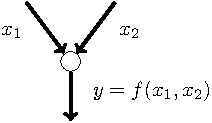
\includegraphics[height=0.15\paperwidth]{../figures/incoming_edges}
\end{figure}
In simple routing, information is transmitted from the source to receivers
through a chain of \textit{intermediate nodes} by a method known as
store-and-forward \cite{Yeung:2006}. In this method, the information
transmission can be represented as \textit{packet transmission}s on
links and the packets received from an incoming link of an intermediate
node, i.e. \textit{incoming packets}, can only be forwarded to a next
node via an outgoing link as its \textit{outgoing packets}. \textit{Network
coding} was though first introduced in Ahlswede et al.'s seminal paper
\cite{Ahlswede:2000} as ``coding at a node in a network'', where
coding means an arbitrary combination of received packets on a node's
incoming links for an outgoing packet. It means that each intermediate
node in the network (not only at the source) is allowed to forward
a \textit{function} of their incoming packets, e.g. $y_{1}=f_{1}(o_{1},o_{2})$
in Figure \ref{fig:incoming_links}. These functions are not required
to be injective functions, i.e. some outgoing packets can be duplicated
from a map of same incoming packets, which motivates our study in
Section \ref{sec:Network_e1l1h3rs4}. A \textit{network code} is a
set of these functions of the packets on the links of the network
\cite{Wachter-Zeh:2018}. A network code is called a \textit{solution}
for the network or the network is \textit{solvable}, if there exists
an assignment of all the functions on all the links of the network
such that each receiver can recover its requested packets from its
incoming packets. If these functions are linear, we obtain a \textit{linear
network coding solution}, and we do not consider \textit{nonlinear
solution} throughout this thesis. Each function on a link consists
of \textit{coding coefficients} for each incoming packet. The coding
coefficients form a coefficient vector whose length is equal to the
number of each node's incoming links, and this coefficient vector
is called the \textit{local coding vector}, which is distinguished
with \textit{global coding vector} defined in Section \ref{subsec:Matrix-channel}.
If the coding coefficients and the packets are scalars, a solution
of linear network coding is called \textit{scalar solution}. Based
on these coding coefficients, K\"otter and M\'edard provided in
\cite{Koetter:2003} an algebraic formulation for the linear network
coding problem and its scalar solvability.

\section{Advantages of Network Coding \label{sec:Advantages-of-NC}}

\paragraph{Throughput gain and reduced complexity}

Network coding gives a potential gain in throughput by communicating
more information with fewer packet transmissions compared to the routing
method. The butterfly network in \cite{Ahlswede:2000} as a multicast
in a wireline network is a standard example for an increase of throughput.
\begin{figure}[H]
\caption{The butterfly network \label{fig:The-butterfly-network}}

\centering{}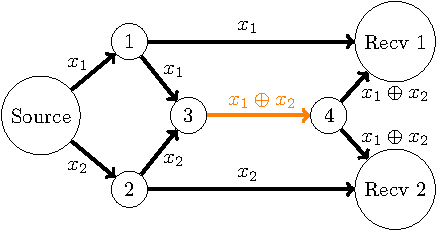
\includegraphics[width=0.5\paperwidth]{../figures/ahlswede_butterfly_network}
\end{figure}
In Figure \ref{fig:The-butterfly-network}, we denoted a receiver
by ``Recv'', which is used for all of figures in this study. With
the help of network coding, both Recv 1 and Recv 2 can recover $x_{1}$
and $x_{2}$ by a bitwise XOR in Figure \ref{fig:The-butterfly-network}(c).
Without network coding, an additional transmission between Node 3
and 4 must be supplemented to communicate the contents of 2 packets
$x_{1}$ and $x_{2}$ from the source to Recv 1 and Recv 2, i.e. we
must communicate $x_{1}$ or $x_{2}$ separately on this link twice
under routing in Figure \ref{fig:The-butterfly-network}(a) and (b). 

\paragraph{Robustness and security}

\textit{Packet loss} is a particular issue in wireless packet networks
due to several reasons, e.g. buffer overflow or communication failures
\cite{Ho:2008}. Sharing a common concept with Erasure Coding (EC)
by exploiting a degree of redundancy to original packets on any nodes
in a network, the receivers are able to successfully recover the original
packets from a large number of packet losses, e.g. $101\circledast10\circledast1$.
The only difference is that packets are only encoded by the source
in EC \cite{Fujimura:2008}. This problem is dealed by acknowledgement
messages in the mechanism of transmission control protocol (TCP) \cite{Ho:2008}.
Network coding offers both benefits and drawbacks regarding to security.
For example, node 4 is operated by an eavesdropper and it obtains
only the packet $x_{1}\oplus x_{2}$, so it cannot obtain either $x_{1}$
or $x_{2}$ and the communication is secure. Alternatively, if the
eavesdropper controls node 3, it can anonymously send a fake packet
masquerading as $x_{1}\oplus x_{2}$, which is difficult to detect
in network coding \cite{Ho:2008}.

\paragraph{From scalar network coding to vector network coding}

Ebrahimi and Fragouli \cite{Ebrahimi:2011} have extended the algebraic
approach in \cite{Koetter:2003} to \textit{vector network coding}.
Here, all packets are vectors of length $t$, and the coding coefficients
are $\left[t\times t\right]$ matrices. The network code is therefore
a set of functions consisting of $\left[t\times t\right]$ coding
matrices, and is called \textit{vector solution} if all receivers
can recover their requested information for such coding marices. The
motivation of vector netwok coding is that there exists networks do
not have scalar solutions, but are solvable by vector routing, e.g
\cite{Medard:2003}. Although it was shown that not every solvable
network has a vector solution in \cite[Lemma II.2]{Dougherty:2005},
Das and Rai proved in \cite{Das:2016} that there exists a network
with a vector solution of dimension $m$ but with no vector solution
over any finite field whose the dimension is less than $m$. When
we refer the \textit{alphabet size} of a network coding solution,
we mean the field size $q_{\mathrm{s}}$ or $q_{v}$ of the finite
field $\ensuremath{\mathbb{F}}_{q_{\mathrm{s}}}$ or $\ensuremath{\mathbb{F}}_{q_{v}}$
respectively for such a scalar solution or a vector solution. The
alphabet size is an important parameter determining the amount of
computation performed at each network node \cite{Wachter-Zeh:2018}.
The problem of finding the minimum required alphabet size of a (linear
or nonlinear) scalar network code for a certain multicast network
is NP-complete \cite{Langberg:2009,Lehman:2004,Gone:2018}. This thesis
focuses on determining the sovability of networks to measure the gap,
and our considered networks in Section \ref{sec:Description_GCN}
consist only error-free links, we therefore do not consider error
correction here. Furthermore, we consider the solvability of networks
by proving an existence of an assignment for all functions such that
all receiver can recover its requested information, so the functions
or coding coefficients are clearly chosen instead of being arbitrary
or random as the ones mentioned in \cite{Ho:2003,Ahlswede:2000}.
We later distinguish scalar and vector network coding more specifically
in Section \ref{subsec:Matrix-channel} and \ref{sec:Network-Coding-for-GCN}.

\section{Network as a Matrix Channel \label{subsec:Matrix-channel}}

To formulate a network coding problem, the source has a set of disjoint
messages referred to packets on links which are either symbols from
$\ensuremath{\mathbb{F}}_{q_{\mathrm{s}}}$ (scalar coding) or vectors
of length $t$ over $\ensuremath{\mathbb{F}}_{q}$ (vector coding)
as mentioned in Section \ref{sec:What-is-NC}. Each receiver $R_{j},j\in\left\{ 1,\ldots,N\right\} $
requests a subset of same $h$ messages from the source. Through all
the functions on the links from the source to each receiver, the receiver
obtains several linear combinations of the $h$ messages to form a
linear system of equations for its requested messages. The coefficients
of a linear combination is called \textit{global coding vector} \cite{Sanders:2003}.
The linear equation system that any receiver $R_{j}$ has to solve
is as following:
\begin{equation}
\begin{array}{c|c}
\mathrm{Scalar} & \mathrm{Vector}\\
\underset{\ensuremath{\mathbb{F}}_{q_{\mathrm{s}}}^{s}}{\underbrace{\left[\begin{array}{c}
y_{j}^{\left(1\right)}\\
\vdots\\
y_{j}^{\left(s\right)}
\end{array}\right]}}=\underset{\ensuremath{\mathbb{F}}_{q_{\mathrm{s}}}^{s\times h}}{\underbrace{\boldsymbol{A}_{j}}}\cdot\underset{\ensuremath{\mathbb{F}}_{q_{s}}^{h}}{\underbrace{\left[\begin{array}{c}
x_{1}\\
\vdots\\
x_{h}
\end{array}\right]}} & \underset{\ensuremath{\mathbb{F}}_{q}^{st}}{\underbrace{\left[\begin{array}{c}
\boldsymbol{y}_{j}^{\left(1\right)}\\
\vdots\\
\boldsymbol{y}_{j}^{\left(s\right)}
\end{array}\right]}}=\underset{\ensuremath{\mathbb{F}}_{q}^{st\times th}}{\underbrace{\boldsymbol{A}_{j}}}\cdot\underset{\ensuremath{\mathbb{F}}_{q}^{th}}{\underbrace{\left[\begin{array}{c}
\boldsymbol{x}_{1}\\
\vdots\\
\boldsymbol{x}_{h}
\end{array}\right]}}
\end{array}\label{eq:linear_system}
\end{equation}
The transfer matrix $\boldsymbol{A}_{j}$ contains the links' global
coding vectors, which are combined by the coefficients of linear combinations
on $\alpha l$ links from $\alpha$ nodes and $\epsilon$ direct-links
to the corresponding receiver $R_{j}$:
\[
\begin{array}{c|c}
\mathrm{Scalar} & \mathrm{Vector}\\
\boldsymbol{A}_{j}=\left[\begin{array}{c}
\boldsymbol{a}^{\left(r_{1}\right)}\\
\vdots\\
\boldsymbol{a}^{\left(r_{\alpha l}\right)}\\
\boldsymbol{b}^{\left(\epsilon\left(j-1\right)+1\right)}\\
\vdots\\
\boldsymbol{b}^{\left(\epsilon j\right)}
\end{array}\right] & \boldsymbol{A}_{j}=\left[\begin{array}{c}
\boldsymbol{A}^{\left(r_{1}\right)}\\
\vdots\\
\boldsymbol{A}^{\left(r_{\alpha l}\right)}\\
\boldsymbol{B}^{\left(\epsilon\left(j-1\right)+1\right)}\\
\vdots\\
\boldsymbol{B}^{\left(\epsilon j\right)}
\end{array}\right]
\end{array}
\]
In general, the network is represented as a matrix channel for both
scalar and vector coding: $\boldsymbol{Y}_{j}=\boldsymbol{A}_{j}\cdot\boldsymbol{X}$.
In our study, the network structure is known, i.e. we reconstruct
$\boldsymbol{X}$ with knowing $\boldsymbol{A}_{j}$, so our network
is coherent. A network is \textit{sovable} or a network code is a
\textit{solution}, if each receiver can reconstruct its requested
messages or solve the system with a unique solution for scalars $x_{1},\ldots,x_{h}$,
or vectors $\boldsymbol{x}_{1},\ldots,\boldsymbol{x}_{h}$. In network
coding problems, we want to find global coding vectors such that the
matrix $\boldsymbol{A}_{j}$ has full-rank for every $j=1,\ldots,N$,
and such that $q_{\mathrm{s}}$ or $q^{t}$ is minimized as mentioned
in Section \ref{sec:Advantages-of-NC}. In Example \ref{ex:scalar_vector_mapping},
we provide a vector solution of field size $q$ and dimension $t$,
which has the same alphabet size as a scalar solution of field size
$q^{t}$.

To summarize the notations of both scalar and vector coding, we represent
them as in Table~\ref{tab:notations}:
\begin{table}[H]
\caption{Notations of network coding \label{tab:notations}}

\centering{}%
\begin{tabular}{|>{\centering}p{0.2\paperwidth}|c|c|}
\hline 
 & Scalar Coding & Vector coding\tabularnewline
\hline 
\hline 
Source Messages/Packets & $\begin{array}{c}
x_{1},\ldots,x_{h}\in\ensuremath{\mathbb{F}}_{q_{\mathrm{s}}}\\
\boldsymbol{x}\in\ensuremath{\mathbb{F}}_{q_{\mathrm{s}}}^{h}
\end{array}$ & $\begin{array}{c}
\boldsymbol{x}_{1},\ldots,\boldsymbol{x}_{h}\in\ensuremath{\mathbb{F}}_{q}^{t}\\
\boldsymbol{x}\in\ensuremath{\mathbb{F}}_{q}^{th}
\end{array}$\tabularnewline
\hline 
Global Coding Vectors Of Receiver $R_{j}$ & $\begin{array}{c}
\boldsymbol{a}^{\left(r_{1}\right)},\ldots,\boldsymbol{a}^{\left(r_{\alpha l}\right)}\in\ensuremath{\mathbb{F}}_{q_{\mathrm{s}}}^{h}\\
\boldsymbol{b}^{\left(\epsilon\left(j-1\right)+1\right)},\ldots,\boldsymbol{b}^{\left(\epsilon j\right)}\in\ensuremath{\mathbb{F}}_{q_{\mathrm{s}}}^{h}
\end{array}$ & $\begin{array}{c}
\boldsymbol{A}^{\left(r_{1}\right)},\ldots,\boldsymbol{A}^{\left(r_{\alpha l}\right)}\in\ensuremath{\mathbb{F}}_{q}^{t\times th}\\
\boldsymbol{B}^{\left(\epsilon\left(j-1\right)+1\right)},\ldots,\boldsymbol{B}^{\left(\epsilon j\right)}\in\ensuremath{\mathbb{F}}_{q}^{t\times th}
\end{array}$\tabularnewline
\hline 
Transfer Matrix Of Receiver $R_{j}$ & $\boldsymbol{A}_{j}\in\ensuremath{\mathbb{F}}_{q_{\mathrm{s}}}^{s\times h}$ & $\boldsymbol{A}_{j}\in\ensuremath{\mathbb{F}}_{q}^{st\times th}$\tabularnewline
\hline 
Packets On Receiver $R_{j}$ & $\begin{array}{c}
y_{j}^{\left(1\right)},\ldots,y_{j}^{\left(s\right)}\in\ensuremath{\mathbb{F}}_{q_{\mathrm{s}}}\\
\boldsymbol{y}_{j}\in\ensuremath{\mathbb{F}}_{q_{\mathrm{s}}}^{s}
\end{array}$ & $\begin{array}{c}
\boldsymbol{y}_{j}^{\left(1\right)},\ldots,\boldsymbol{y}_{j}^{\left(s\right)}\in\ensuremath{\mathbb{F}}_{q}^{t}\\
\boldsymbol{Y}_{j}\in\ensuremath{\mathbb{F}}_{q}^{st}
\end{array}$\tabularnewline
\hline 
Number of nodes & $r_{\mathrm{scalar}}$ & $r_{\mathrm{vector}}$\tabularnewline
\hline 
\end{tabular}
\end{table}

\begin{rem}
By using the vector coding, the upper bound number of solutions increases
from $q^{tsh}$ to $q^{t^{2}sh}$. Therefore, vector network coding
offers more freedom in choosing the coding coefficients than does
scalar linear coding for equivalent alphabet sizes, and a smaller
alphabet size might be achievable \cite{Ebrahimi:2011}. By this advantage,
we can have higher number of receivers, i.e. higher number of nodes,
in vector network coding.
\end{rem}

\section{Network Model}

\subsection{Multicast Networks as Generalized Combination Networks}

A class of networks which is mainly studied is the class of multicast
networks. It can be one-to-many or many-to-many distribution \cite{Harte:2008}.
In this study, we target one-to-many multicast network with the distribution
of a data packet to a group of users \cite{Zhang:2012}. An interesting
network structure often used for multicast networks in network coding
is called Combination Network (CN) and denoted by $\mathcal{N}_{h,r,s}$.
Many examples in previous studies demonstrating the advantage of network
coding have used structures identical or similar to that of CN. We
mention a few examples to emphasize CN's importance in the study of
network coding. In Figure \ref{fig:butterfly_nw_cn}, the butterfly
network that is often used as a first example to motivate network
coding, e.g. \cite[Fig. 7]{Ahlswede:2000} and \cite[Fig. 1]{Sanders:2003},
is isomorphic to $\mathcal{N}_{h,r=3,s=2}$, if we consider it as
an undirected network \cite{Maheshwar:2012}. The $\mathcal{N}_{h,r=3,s=2}$
itself was also used in the first study of network coding \cite{Ahlswede:2000}.
Other CNs, i.e. $\mathcal{N}_{h,r=4,s=2}$ and $\mathcal{N}_{h,r=6,s=3}$,
were also used as examples to demonstrate the advantage of network
coding in \cite[Fig. 2]{Sanders:2003} and \cite[Fig. 2]{Jaggi:2005}
respectively. The general structure of CN was also introduced and
discussed in \cite[Sec. 4.3]{Fragouli:2006}, \cite[Sec. 4.1]{Yeung:2006},
\cite{Ngai:2004,Xiao:2007}.
\begin{figure}[H]
\caption{The butterfly network is represented as a combination network \label{fig:butterfly_nw_cn}}

\centering{}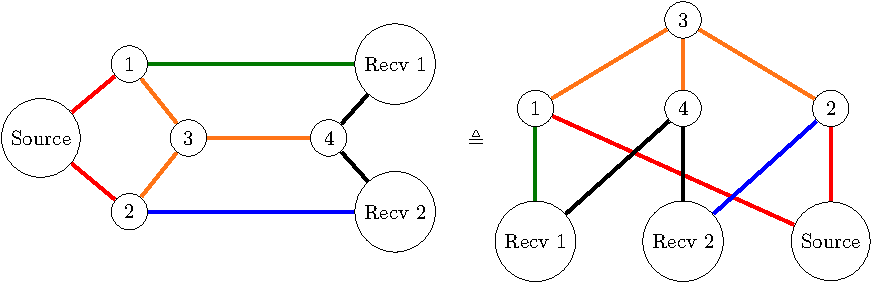
\includegraphics[width=0.5\paperwidth]{../figures/ahlswede_butterfly_network_CN}
\end{figure}
A generalization of a CN \cite{Riis:2006} is called generalized combination
network (GCN). GCN defined in \cite{Etzion:2016,Wachter-Zeh:2018}
was used to prove that vector network coding outperforms scalar linear
network coding , in multicast networks, with respect to the \textit{alphabet
size}, using rank-metric codes and Grassmannian codes. A comparison
between the required alphabet size for a scalar linear solution, a
vector solution, and a scalar nonlinear solution, of the same multicast
network is an important problem. Etzion and Wachter-Zeh introduced
a \textit{gap} in \cite{Etzion:2016} as the difference between the
smallest alphabet size for which a scalar linear solution exists and
the smallest alphabet size for which they can construct a vector solution.
They have found bounds on the gap for several network families of
GCN in \cite{Etzion:2016,Wachter-Zeh:2018}, but no gap for the GCN
networks with 3 messages has been found, i.e. $(1,1)-\mathcal{N}_{3,r,4}$,
where we denote GCN by $(\epsilon,l)-\mathcal{N}_{h,r,s}$. Therefore,
a combinatorial approach is first introduced in this thesis to prove
an existence of a vector solution outperforming the optimal scalar
linear solution with $q^{t^{2}/4+\mathcal{O}(t)}$. We then further
extend the approach for a family of GCN called One-Direct Link Combination
Network, i.e. $(1,1)-\mathcal{N}_{h,r,s}$. More formal definitions
of the gap and GCN can be found in Section \ref{sec:Description_GCN}.

\subsection{Comparison between Scalar and Vector Solutions by the Gap Size \label{subsec:Comparison-between-scalar-and-vector-sol}}

A \textit{gap} represents the difference between the smallest field
(alphabet) size for which a scalar linear solution exists and the
smallest alphabet size for which we can construct a vector solution.
In this study, we define a solvable vector network coding over the
field size $\ensuremath{\mathbb{F}}_{q}^{t}$, and we find the lower
bound of the maximum number of nodes such vector solution can achieve,
i.e. $r_{\mathrm{max,vector}}=f_{\mathrm{1}}(q,t,\alpha,h)\geq f_{\mathrm{1,lower\,bound}}\left(q,t,\alpha,h\right)$,
with $f_{\mathrm{1}}:\mathbb{Z}\rightarrow\mathbb{Z}$. Meanwhile,
we have a scalar solution for the same network existing if and only
if $r\leq r_{\mathrm{max,scalar}}=f_{\mathrm{2}}\left(q_{\mathrm{s}}\right)\leq f_{\mathrm{2,upper\,bound}}\left(q_{\mathrm{s}}\right)$,
with $f_{\mathrm{2}}:\mathbb{Z}\rightarrow\mathbb{Z}$. To find the
field size $q_{\mathrm{s}}$ required for a scalar solution to reach
the maximum achievable vector solution's nodes in this setting, we
consider $r_{\mathrm{max,scalar}}=f_{\mathrm{2}}\left(q_{\mathrm{s}}\right)=f_{\mathrm{1}}(q,t,\alpha,h)=r_{\mathrm{max,vector}}$
and express $q_{\mathrm{s}}$ in term of $q,t,\alpha,h$. In other
words, we compute such field size as following, $q_{\mathrm{s}}\left(q,t,\alpha,h\right)=\mathrm{\mathrm{min}\left\{ q_{\mathrm{s}}:f_{\mathrm{2}}\left(q_{\mathrm{s}}\right)\geq f_{\mathrm{1}}\left(q,t,\alpha,h\right)\right\} }$,
we then calculate the gap by $g=q_{\mathrm{s}}-q_{v}=q_{\mathrm{s}}-q^{t}$,
which is similar to the way to compute the gap in \cite{Wachter-Zeh:2018}.
In this thesis, we focus on a lower bound of the gap as following,
\[
g\geq g_{\mathrm{lower\,bound}}=q_{\mathrm{s,min,from\,bound}}(q,t,\alpha,h)-q^{t}
\]

, where $q_{\mathrm{s,min,from\,bound}}=\mathrm{min}\left\{ q_{\mathrm{s}}:f_{\mathrm{2,upper\,bound}}\left(q_{\mathrm{s}}\right)\geq f_{\mathrm{1,lower\,bound}}\left(q,t,\alpha,h\right)\right\} $. 

Throughout this study, we show that vectors solutions significantly
reduce the required alphabet size by the lower bound of the gap denoted
by $g_{\mathrm{lower\,bound}}$.

\part{Generalized Combination Network }

\section{Description \label{sec:Description_GCN}}

A generalized combination network $(\epsilon,\ell)-\mathcal{N}_{h,r,s}$
consists of 3 components over 3 layers from top to bottom: ``Source''
in the first layer, ``Intermediate Nodes'' in the middle layer,
and ``Receiver'' in the third layer. Because ``Source'' and ``Receiver''
have their own names without previous confusion of a source node or
a destination node, we replace ``Intermedate Nodes'' by ``Nodes''
from this section. The network has a source with $h$ messages, $r$
nodes, and $\left(\begin{array}{c}
r\\
\alpha
\end{array}\right)$ receivers, which form a single source multicast network modeled as
a finite directed acyclic multigraph \cite{Li:2003,Riis:2006,Wachter-Zeh:2018}.
The source connects to each node by $\ell$ parallel links and each
node also connects to a receiver by $\ell$ parallel links, which
are respectively called a node's incoming and outgoing links. Each
receiver is connected by $s$ links in total, specifically $\alpha l$
links from $\alpha$ nodes and $\epsilon$ direct links from the source,
i.e. $s=\alpha\ell+\epsilon$. The combination network in \cite{Riis:2006}
is the $(0,1)-\mathcal{N}_{h,r,s}$ network and the $(1,1)-\mathcal{N}_{h,r,s}$
network is called One-Direct Link Combination Network. Theorem 1 shows
our interest of relations between the parameters $h,\alpha,\epsilon$
and $\ell$. Following to Theorem \ref{nw_parameters}, we are interested
in networks parameters satisfying this condition: $\ell+\epsilon+1\leq h\leq\alpha\ell+\epsilon$.
\begin{figure}[H]
\caption{The generalized network $(\epsilon,\ell)-\mathcal{N}_{h,r,s}$\label{fig:The-generalized-network}}

\centering{}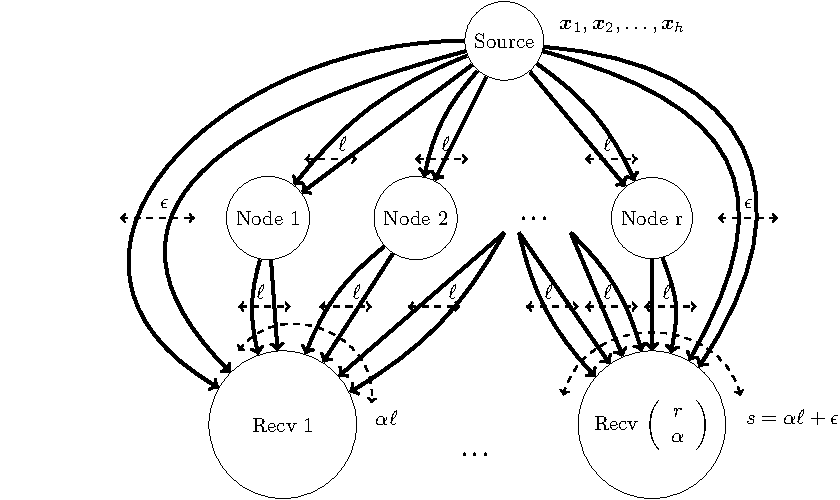
\includegraphics[width=0.5\paperwidth]{../figures/generalized_combination_nw}
\end{figure}

\begin{thm}[\cite{Wachter-Zeh:2018}]
\label{nw_parameters}The $(\epsilon,\ell)-\mathcal{N}_{h,r,s}$
network has a trivial solution if $\ell+\epsilon\geq h$, and it has
no solution if $\alpha\ell+\epsilon<h$.
\end{thm}
\begin{proof}
Following to the network coding max-flow min-cut theorem for multicast
networks, the maximum number of messages from the source to each receiver
is equal to the smallest min-cut between the source and any receiver.
For our considered network, $s$ links have to be deleted to disconnect
the source from the receiver, which implies that the min-cut between
the source and each receiver is at least $s$. Hence, $h\leq s\Leftrightarrow h\leq\alpha\ell+\epsilon$. 

There exist at least $\ell+\epsilon$ disjoint links connected to
each receiver. If $\ell+\epsilon\geq h$, each receiver can always
reconstruct its requested messages on its links. Then we only need
to do routing to select paths for the network.
\end{proof}
\begin{table}[H]
\caption{Parameters of network coding \label{tab:Parameters-of-network}}

\centering{}%
\begin{tabular}{|c|>{\centering}p{0.48\paperwidth}|}
\hline 
$h$ & The number of source messages\tabularnewline
\hline 
$r$ & The number of nodes in the middle layer\tabularnewline
\hline 
$\left(\begin{array}{c}
r\\
\alpha
\end{array}\right)$ & The number of receivers\tabularnewline
\hline 
$\ell$ & The source connects to each node by $\ell$ parallel links, and each
node also connects to one receiver by $\ell$ parallel links\tabularnewline
\hline 
$\alpha$ & A receiver is connected by any $\alpha$ nodes in the middle layer\tabularnewline
\hline 
$\epsilon$ & The source additionally connects to each receiver by $\epsilon$ direct
parallel links\tabularnewline
\hline 
$s$ & Each receiver is connected by $s$ links in total, with $s=\alpha\ell+\epsilon$.\tabularnewline
\hline 
\end{tabular}
\end{table}


\section{Network Coding for the Generalized Combination Network \label{sec:Network-Coding-for-GCN}}

Network coding in general was described in Section \ref{sec:What-is-NC}
and Section \ref{subsec:Matrix-channel}. Now, we start describing
a difference of a source message used in scalar network coding and
vector network coding. Then we find a condition for an existence of
a scalar solution and a vector solution respectively. For the $(\epsilon,\ell)-\mathcal{N}_{h,r,s}$
network, the \textit{local} and \textit{global} coding vectors are
the same, because the nodes are simplified to forward their received
packets and only the source has its functions on its messages.

\subsection{Scalar Network Coding \label{subsec:Scalar-network-coding}}

A message or a packet is equivalent to a symbol over $\ensuremath{\mathbb{F}}_{q_{\mathrm{s}}},$which
was introduced in Table \ref{tab:notations}. As a network of the
multicast model, all receivers request the same $h$ symbols at the
same time \cite{Trautmann:2013}. A transmission of $h$ data units
is a 1-dimentional subspace of $\ensuremath{\mathbb{F}}_{q_{\mathrm{s}}}^{h}$.
Each receiver therefore must obtain a subspace of $\ensuremath{\mathbb{F}}_{q_{\mathrm{s}}}^{h}$,
whose dimension is at least $h$, to be able to reconstruct the packet.
Through $\epsilon$ direct links connected from the source to a receiver,
the source can provide any required $\epsilon$ 1-dimensional subspaces
of $\ensuremath{\mathbb{F}}_{q_{\mathrm{s}}}^{h}$ for the corresponding
receiver. Each receiver can accordingly reconstruct the packet if
and only if the linear span of $\alpha$ $\ell$-dimensional subspaces
of $\ensuremath{\mathbb{F}}_{q_{\mathrm{s}}}^{h}$ from the nodes
is at least of dimension $h-\epsilon$. When this necessary condition
is satisfied, the network is said to have a \textit{solution} or to
be \textit{solvable}, which was briefly introduced in Section \ref{sec:What-is-NC}.
\begin{thm}[\cite{Riis:2006}]
 The $(0,1)-\mathcal{N}_{h,r,s}$ network has a solution if and only
if there exists an $\left(r,\left|\ensuremath{\mathbb{F}}_{q_{\mathrm{s}}}\right|h,r-\alpha+1\right)$
$\left|\ensuremath{\mathbb{F}}_{q_{\mathrm{s}}}\right|$-ary error
correcting code. 
\end{thm}
%
\begin{thm}[\cite{Zhang:2019}]
 The $(\epsilon,\ell)-\mathcal{N}_{h,r,s=\alpha l+\epsilon}$network
is solvable over $\ensuremath{\mathbb{F}}_{q}$ if and only if there
exists an $\alpha-\left(h,\ell,h-\ell-\epsilon\right)_{q}^{c}$ code
with $r$ codewords. \label{theo:scalar_sol_exist}
\end{thm}

\subsection{Vector Network Coding \label{subsec:Vector-network-coding}}

In vector network coding, a message or a packet is a vector of length
$t$ over $\ensuremath{\mathbb{F}}_{q}$. A vector solution is therefore
over field size $q$ and dimension $t$. Such a vector solution has
the same alphabet size as a scalar solution of field size $q^{t}$,
and we denote $q_{v}=q^{t}$. A mapping from the scalar solution of
field size $q^{t}$ to an equivalent vector solution is represented
in Example \ref{ex:scalar_vector_mapping}. Similarly with the scalar
\textit{linear} coding solution, each receiver can reconstruct its
requested packet if and only if any $\alpha$ $\left(\ell t\right)$-dimensional
subspaces span a subspace of dimension at least $\left(h-\epsilon\right)t$.
\begin{thm}[\cite{Zhang:2019}]
 A vector solution for the $(\epsilon,\ell)-\mathcal{N}_{h,r,s}$
network exists if and only if there exists $\mathcal{G}_{q}\left(ht,\ell t\right)$
such that any $\alpha$ subspaces of the set span a subspace of dimension
at least $\left(h-\epsilon\right)t$. 
\end{thm}
%
\begin{thm}[\cite{Zhang:2019}]
 The $(\epsilon,\ell)-\mathcal{N}_{h,r,s=\alpha\ell+\epsilon}$network
is solvable with vectors of length $t$ over $\ensuremath{\mathbb{F}}_{q}$
if and only if there exists an $\alpha-\left(ht,\ell t,ht-\ell t-\epsilon t\right)_{q}^{c}$
code with $r$ codewords. 
\end{thm}
\begin{cor}
The $\alpha-\left(n=ht,n-k=ht-\ell t,\lambda=ht-\ell t-\epsilon t\right)_{q}^{m}$
code formed from the dual subspaces of the $\alpha-\left(n=ht,k=\ell t,\lambda=ht-\ell t-\epsilon t\right)_{q}^{c}$
code yields the upper bound of $\mathcal{A}_{q}\left(n=ht,n-k=ht-\ell t,\alpha;\lambda\right)$
as maximum number of nodes for a vector network coding of the $(\epsilon,\ell)-\mathcal{N}_{h,r,s}$
network. \label{cor:dual_subspaces}
\end{cor}
\begin{example}
\label{ex:scalar_vector_mapping} 

Given $h=3,q=2,t=2$, we consider the extension field $\ensuremath{\mathbb{F}}_{q^{t}=2^{2}}$.
This example shows how mapping messages from scalar coding to vector
coding.
\begin{figure}[H]
\caption{The mapping of a scalar solution over $\ensuremath{\mathbb{F}}_{q_{\mathrm{s}}=q^{t}}$
to an equivalent vector solution\label{fig:x_mapping}}

\centering{}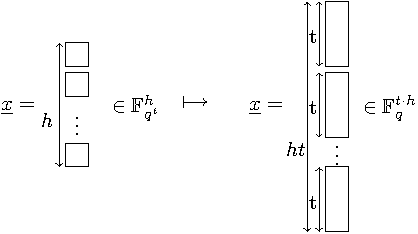
\includegraphics[width=0.3\paperwidth]{../figures/x_mapping}
\end{figure}
\end{example}
We use the table of the extension field $\ensuremath{\mathbb{F}}_{2^{2}}$
with the primitive polynomial $f(x)=x^{2}+x+1$:
\begin{center}
\begin{table}

\caption{The extension field $\ensuremath{\mathbb{F}}_{2^{2}}$}

\centering{}%
\begin{tabular}{|c|c|c|}
\hline 
power of $\alpha$ & polynomial & binary vector\tabularnewline
\hline 
- & 0 & 00\tabularnewline
\hline 
$\alpha^{0}$ & 1 & 01\tabularnewline
\hline 
$\alpha^{1}$ & $\alpha$ & 10\tabularnewline
\hline 
$\alpha^{2}$ & $\alpha+1$ & 11\tabularnewline
\hline 
\end{tabular}
\end{table}
For scalar coding, the messages are $x_{1},\ldots,x_{h=3}\in\ensuremath{\mathbb{F}}_{2^{2}}$
, and for vector coding the messages are $\boldsymbol{x}_{1},\ldots,\boldsymbol{x}_{h=3}\in\ensuremath{\mathbb{F}}_{2}^{2}$.
From the polynomial column, let's choose arbitrarily a scalar vector
$\boldsymbol{x}_{\mathrm{scalar}}=(x_{1},x_{2},x_{3})=(1,\alpha,\alpha+1)$.
Then, we map it to $\boldsymbol{x}_{\mathrm{vector}}=(\boldsymbol{x}_{1},\boldsymbol{x}_{2},\boldsymbol{x}_{3})$
by using the binary vector column as following:
\[
\left[\begin{array}{c}
x_{1}=1\\
x_{2}=\alpha\\
x_{3}=\alpha+1
\end{array}\right]\rightarrow\left[\begin{array}{c}
\left(\begin{array}{c}
1\\
0
\end{array}\right)\\
\left(\begin{array}{c}
0\\
1
\end{array}\right)\\
\left(\begin{array}{c}
1\\
1
\end{array}\right)
\end{array}\right],
\]
\par\end{center}

where we use the following rule for mapping $x_{i}$ individually:
$a_{0}\cdot\alpha^{0}+a_{1}\cdot\alpha^{1}+\ldots+a_{t-1}\cdot\alpha^{t-1}\rightarrow\left(\begin{array}{c}
a_{0}\\
a_{1}\\
\vdots\\
a_{t-1}
\end{array}\right)$.

\section{Instances of Generalized Combination Network}

This subsection lists all instances of the $(\epsilon,\ell)-\mathcal{N}_{h,r,s}$
network used by Etzion and Wachter-Zeh in \cite{Wachter-Zeh:2018}
to derive gaps between scalar and vector network coding. They cover
some extreme values of the pair $(\epsilon,\ell)$, i.e. $(\epsilon=0,\ell=1)$,
$(\epsilon=1,\ell)$, $(\epsilon,\ell=1)$ and $(\epsilon=l-1,\ell)$.
In Section \ref{sec:e1l1_nw}, we further study these interesting
cases $(\epsilon=1,\ell=1)$, $(\epsilon>1,\ell=1)$ and $(\epsilon=1,\ell>1)$.
In Table \ref{tab:New-gap-found}, we show our newly found gaps and
compare our gaps with known gaps found in \cite{Wachter-Zeh:2018}.

\subsection{The $(\ell-1)$-Direct Links and $\ell$-Parallel Links $\mathcal{N}_{h=2l,r,s=3l-1}$
Network}

This network family is denoted by $\left(\ell-1,\ell\geq2\right)-\mathcal{N}_{2\ell,r,3\ell-1}$.
This family contains the largest number of direct links from the source
to the receivers among all families of GCN. Its vector solution can
be provided by an $\mathcal{MRD}\left[\ell t\times\ell t,t\right]_{q}$
code for any $r_{\mathrm{vector}}\leq q^{\ell\left(\ell-1\right)t^{2}+\ell t}$.
There is a scalar solution for this network, if and ony if $r_{\mathrm{scalar}}\leq\left[\begin{array}{c}
2\ell\\
\ell
\end{array}\right]_{q_{s}}<4_{q_{s}}^{\ell^{2}}$. Therefore, the gap tends to $q^{t^{2}+\mathcal{O}\left(t\right)}$
for large $\ell$.
\begin{figure}[H]
\caption{The $\left(1,2\right)-\mathcal{N}_{4,r,5}$ network as an example
of the $\left(\ell-1,\ell\right)-\mathcal{N}_{2\ell,r,3\ell-1}$ \label{fig:network_l1e2h4rs5}}

\centering{}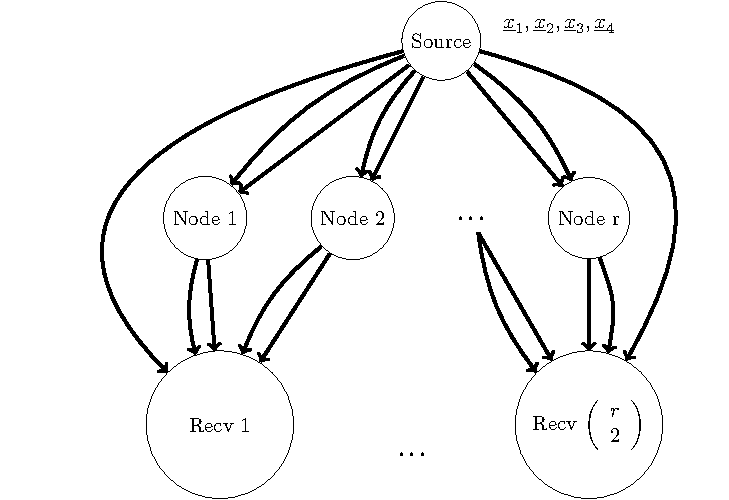
\includegraphics[width=0.4\paperwidth]{../figures/nw_e1_l2_h4_r_s5}
\end{figure}


\subsection{The 1-Direct Link and $\ell$-Parallel Links $\mathcal{N}_{h=2\ell,r,s=2\ell+1}$
Network}

We denote this network family by $(1,\ell\geq2)-\mathcal{N}_{2\ell,r,2\ell+1}$.
This network family is the family with the smallest number of direct
links, such that Etzion and Wachter-Zeh's vector solution outperforms
the optimal scalar solution, i.e. an vector solution outperforming
the optimal scalar has not yet been found for the network $(0,\ell\geq2)-\mathcal{N}_{h,r,s}$.
When $\ell\geq2$ or $h\geq4$, they proved that this network has
a vector solution based on an $\mathcal{MRD}\left[\ell t\times\ell t,(\ell-1)t\right]_{q}$
code when $r=q^{\ell t\left(t+1\right)},$and scalar solutions only
if $q_{s}>q^{t^{2}/2}$. Therefore, this network has a gap tending
to $q^{t^{2}/2+\mathcal{O}\left(t\right)}$ with a vector solution
.
\begin{figure}[H]
\caption{The $\left(\ell-1,\ell\right)-\mathcal{N}_{2\ell,r,3\ell-1}$ network
\label{fig:network_special2}}

\centering{}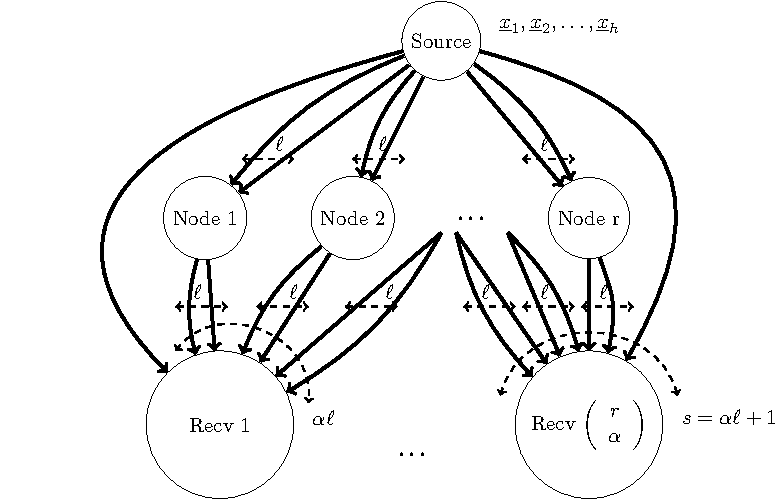
\includegraphics[width=0.45\paperwidth]{../figures/nw_special2}
\end{figure}


\subsection{The $\epsilon$-Direct Links $\mathcal{N}_{h,r,s}$}

This network family is denoted by $\left(\epsilon\geq1,\ell=1\right)-\mathcal{N}_{h,r,s}$
and is the main focus of this thesis, because it motivates some interesting
questions on a classic coding problem and on a new type of subspace
code problem. Furthermore, there is no gap size is known for this
network in previous studies. In Section \ref{sec:Network_e1l1h3rs4},
we show that there exists vector solutions generating the gaps $g=q^{t^{2}/4+\mathcal{O}(t)}$
and $g=q^{\frac{\alpha-h+1}{\left(\alpha-1\right)\left(\alpha-h+2\right)\left(h-2\right)}t^{2}+\mathcal{O}(t)}$
respectively for the $\left(1,1\right)-\mathcal{N}_{3,r,4}$ network
and the $\left(1,1\right)-\mathcal{N}_{h,r,s}$ network. 
\begin{figure}[H]
\caption{The $\left(\epsilon\protect\geq1,\ell=1\right)-\mathcal{N}_{h,r,s}$
network \label{fig:network_special3}}

\centering{}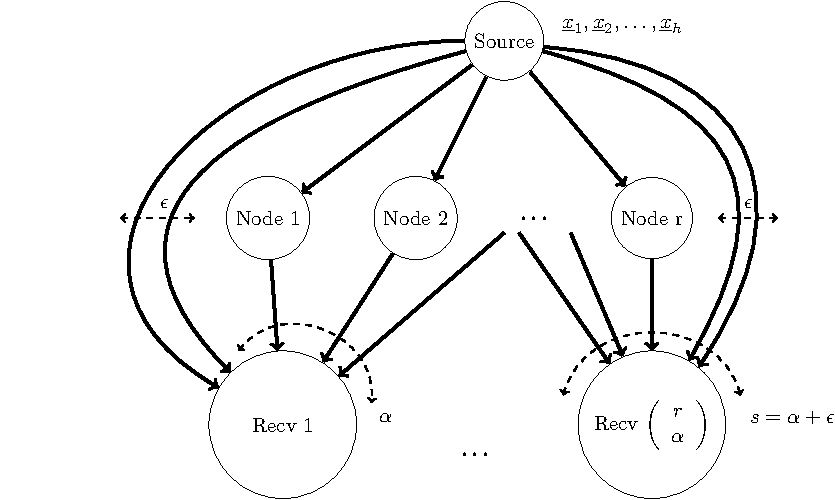
\includegraphics[width=0.45\paperwidth]{../figures/nw_special3}
\end{figure}


\subsection{The $\left(\epsilon=0,\ell=1\right)-\mathcal{N}_{h,r,s}$ Combination
Network}

Since the scalar solution for the combination network uses an $MDS$
code, a vector solution based on subspace codes must go beyond the
$MDS$ bound, i.e. Singleton bound $d\leq n-k+1$, to outperform the
scalar one. In paper \cite[Sec. IV-A, Sec. IX-1,2]{Wachter-Zeh:2018},
it is proved that vector solutions based on subspace codes cannot
outperform optimal scalar linear solutions for some combination networks,
e.g. $\mathcal{N}_{2,r,2}$, and they conjecture it for all $h$.
\begin{figure}[H]
\caption{The $\left(\epsilon=0,\ell=1\right)-\mathcal{N}_{h,r,s}$ combination
network \label{fig:network_special4}}

\centering{}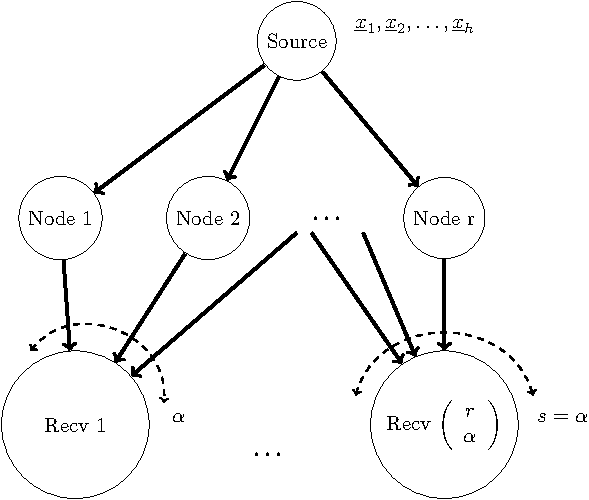
\includegraphics[width=0.4\paperwidth]{../figures/nw_special4_combination}
\end{figure}


\subsection{The Largest Possible Gap between $q_{v}$ and $q_{s}$ in Previous
Studies}

Etzion and Wachter-Zeh distinguished 2 following cases $h\leq2\ell,\epsilon\neq0$
and $h\geq2\ell,\epsilon\neq h-2\ell$.

For $h\leq2\ell$ and $\epsilon\neq0$, the number of direct links
is at least 1 for networks of this case, i.e. $\epsilon\geq1$, and
the number of parallel links is less than half of the number of source
messages, i.e. $\ell\leq\frac{h}{2}$. When $h$ is even, the above
$\left(\ell-1,l\right)-\mathcal{N}_{2\ell,r,3\ell-1}$ network achieves
the largest gap $q_{\mathrm{s}}=q^{(h-2)t^{2}/h+\mathcal{O}(t)}$,
and when $h$ is odd, the $\left(\ell-2,\ell\right)-\mathcal{N}_{2\ell-1,r,3\ell-2}$
network achieves the largest gap $q_{\mathrm{s}}=q^{\left(h-3\right)t^{2}/\left(h-1\right)+\mathcal{O}(t)}$.

For $h\geq2\ell$ and $\epsilon\neq h-2\ell$, when $h$ is even the
same above $\left(\ell-1,\ell\right)-\mathcal{N}_{2\ell,r,3\ell-1}$
network achieves the largest gap $q_{s}=q^{(h-2)t^{2}/h+\mathcal{O}(t)}$,
and when $h$ is odd, the $\left(\ell-1,\ell\right)-\mathcal{N}_{2\ell+1,r,3\ell-1}$
network achieves the largest gap $q_{\mathrm{s}}=q^{(h-3)t^{2}/\left(h-1\right)+\mathcal{O}(t)}$.
\begin{rem}
The achieved gap is $q^{(h-2)t^{2}/h+\mathcal{O}(t)}$ for any $q\geq2$
and any even $h\geq4$. If $h\geq5$ is odd, then the achieved gap
of the alphabet size is $q^{(h-3)t^{2}/\left(h-1\right)+\mathcal{O}(t)}$
\cite{Wachter-Zeh:2018}.
\end{rem}
We are summarizing the instances of GCN with their bounds on gap found
in \cite{Wachter-Zeh:2018} and list our findings in this study.
\begin{table}

\caption{New gaps found in this study\label{tab:New-gap-found}}

\begin{centering}
\begin{tabular}{|>{\centering}p{0.15\paperwidth}|>{\centering}p{0.1\paperwidth}|>{\centering}p{0.2\paperwidth}|}
\hline 
\centering{}Network & \centering{}Gaps for a specific vector solution \cite{Wachter-Zeh:2018}) & \begin{centering}
Lower bounds on gaps 
\par\end{centering}
\centering{}(Corollary \ref{cor:gap_e1l2} and Corollary \ref{cor:e2l1_gap})\tabularnewline
\hline 
\hline 
\centering{}$\left(\epsilon=0,\ell=1\right)-\mathcal{N}_{h,r,s}$ & \centering{}N/A & \centering{}N/A\tabularnewline
\hline 
\centering{}$\left(\epsilon\geq1,\ell=1\right)-\mathcal{N}_{h,r,s}$ & \centering{}N/A & \centering{}$q^{\frac{\epsilon\left(\alpha-h+\epsilon\right)}{\left(\alpha-1\right)\left(\alpha-h+\epsilon+1\right)\left(h-\epsilon-1\right)}t^{2}+\mathcal{O}(t)}$\tabularnewline
\hline 
\begin{centering}
$(\epsilon=1,\ell\geq2)-$
\par\end{centering}
$\mathcal{N}_{h=2\ell,r,s=2\ell+1}$ & \centering{}$q^{t^{2}/2+\mathcal{O}\left(t\right)}$ & \centering{}$q^{t^{2}/l+\mathcal{O}\left(t\right)}$\tabularnewline
\hline 
\begin{centering}
$\left(\epsilon=\ell-1,\ell\right)-$
\par\end{centering}
$\mathcal{N}_{h=2\ell,r,s=3\ell-1}$ & \centering{}$q^{t^{2}/2+\mathcal{O}\left(t\right)}$ & \centering{}N/A\tabularnewline
\hline 
\end{tabular}
\par\end{centering}
\end{table}
Some of them has global coding vectors as square matrices, so a decoding
method for each receiver is easily by inversing such global coding
vectors to get each receiver's requested messages. However, we do
not go into details of decoding methods in this study.

\part{Combinatorial Results}

This section contains new results on gaps of 3 different instances
of the GCN mentioned in Section \ref{sec:Description_GCN}. In previous
studies \cite{Wachter-Zeh:2018}, no general vector solution outperforming
scalar network coding was found for multicast networks with $h=3$
messages. Hence, we start with a probabilistic argument to prove that
there exists a vector solution outperforming the optimal linear solution
for the $\left(\epsilon=1,\ell=1\right)-\mathcal{N}_{h=3,r,s=4}$
network. Our approach is to study the network as a matrix channel
introduced in Section \ref{subsec:Matrix-channel} and apply the Symmetric
Lov\'asz Local Lemma \ref{thm:LLL} (LLL) for the proof. The idea
of this approach for the vector network coding was proposed by Schwartz
\cite{MosheSchwartz:2018} and the optimal scalar linear solution
was studied in \cite{Wachter-Zeh:2018}. We therefore can compute
a gap in alphabet sizes for our vector solutions and the optimal scalar
linear solution in Section \ref{sec:Network_e1l1h3rs4}. 

Then, we generalize the proof to the $\left(\epsilon=1,\ell=1\right)-\mathcal{N}_{h,r,s}$
network, the $\left(\epsilon>1,\ell=1\right)-\mathcal{N}_{h,r,s}$
network and the $\left(\epsilon=1,\ell>1\right)-\mathcal{N}_{h=2\ell,r,s=2\ell+1}$
network. As explained in Section \ref{sec:What-is-NC}, multiple parallel
links $\ell$ of a data unit help us to show networks with large-capacity
transmission between source and receivers. The direct links among
them are not really usual in reality, i.e. a server and a client often
has long-distance connection through multiple intermediate nodes,
it is thus interesting to study networks with $\epsilon=1$ and $l>1$.
By applying rank requirements for each receiver to be able to solve
linear systems in (\ref{eq:linear_system}), we prove that there exists
scalar and vector solutions for such networks if the number $r$ of
intermediate nodes is bounded by a certain number. Then, we can show
gaps of the networks based network parameters $q,t,\alpha,h$. In
this study, we derive lower bounds on such gaps following to Sectioin
\ref{subsec:Comparison-between-scalar-and-vector-sol}, our gap for
the $\left(\epsilon=1,\ell>1\right)-\mathcal{N}_{h=2\ell,r,s=2\ell+1}$
network is thus less than the one found in \cite{Wachter-Zeh:2018}.
However, gaps for the $\left(\epsilon=1,\ell=1\right)-\mathcal{N}_{h,r,s}$
network and the $\left(\epsilon>1,\ell=1\right)-\mathcal{N}_{h,r,s}$
network are not known in any other studies.

We formally use $r_{\mathrm{scalar}}$ and $r_{\mathrm{vector}}$
in Table \ref{tab:Parameters-of-network} to distinguish the $r$
parameter of GCN for scalar solutions and vector solutions to compare
a gap derived from such solutions. Because they both have the same
meaning as a number of intermediate nodes in a network, we use $r$
when we need to state a vector solution or a scalar solution exists
under some conditions of $r$.

\section{$\left(\epsilon=1,\ell=1\right)-\mathcal{N}_{h=3,r,s=4}$ Network
\label{sec:Network_e1l1h3rs4}}

\begin{figure}[H]
\caption{The $(\epsilon=1,\ell=1)-\mathcal{N}_{h=3,r,s=4}$ network\label{fig:nw_e1_l1_h3_r_s4}}

\centering{}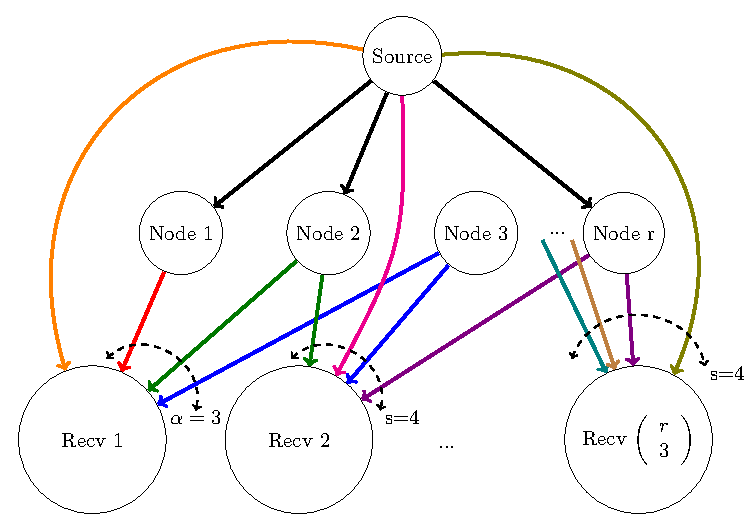
\includegraphics[width=0.5\paperwidth]{../figures/nw_e1_l1_h3_r_s4}
\end{figure}

In this subsection, we derive a lower bound on the maximum number
of receivers for the $\left(\epsilon=1,\ell=1\right)-\mathcal{N}_{h=3,r,s=4}$
network such that a vector solution for the network exists. Due to
$\alpha=3$, the number of receivers is $N=\left(\begin{array}{c}
r\\
3
\end{array}\right)$ by definition in Section \ref{sec:Description_GCN}. A problem of
finding the maximum $N$ is thus equivalent to find a maximum number
of intermediate nodes $r$. We denote the maximum number of such nodes
for a vector solution by $r_{\mathrm{max,vector}}$. Our goal is therefore
to derive $r_{\mathrm{max,vector}}$ such that there exists a vector
solution for the $\left(1,1\right)-\mathcal{N}_{3,r,4}$ network for
any $r\leq r_{\mathrm{max,vector}}$. In \cite[Section VIII.C]{Wachter-Zeh:2018},
Etzion and Wachter-Zeh stated that there exists a scalar solution
for the network for any $r\leq r_{\mathrm{max,scalar}}$ with $r_{\mathrm{max,scalar}}=2\left(q_{s}^{2}+q_{s}+1\right)$.
Based on $r_{\mathrm{max,scalar}}$ and $r_{\mathrm{max,vector}}$,
we then calculate the gap in alphabet sizes for such scalar and vector
solutions of the $\left(1,1\right)-\mathcal{N}_{3,r,4}$ network following
to Section \ref{subsec:Comparison-between-scalar-and-vector-sol}.
To discuss the vector solvability of the network, we introduce a rank
requirement on the transfer matrix $\boldsymbol{A}_{j}$ corresponding
to each receiver $R_{j}$. In Figure \ref{fig:nw_e1_l1_h3_r_s4},
each receiver $R_{j}$ obtains 4 linear combinations of the 3 source
messages. In other words, the transfer matrix $\boldsymbol{A}_{j}$
maps the messages $x_{1},x_{2},x_{3}$ to $y_{j}^{\left(1\right)},y_{j}^{\left(2\right)},y_{j}^{\left(3\right)},y_{j}^{\left(4\right)}$
or $\boldsymbol{x}_{1},\boldsymbol{x}_{2},\boldsymbol{x}_{3}$ to
$\boldsymbol{y}_{j}^{\left(1\right)},\boldsymbol{y}_{j}^{\left(2\right)},\boldsymbol{y}_{j}^{\left(3\right)},\boldsymbol{y}_{j}^{\left(4\right)}$
respectively regarding to scalar or vector network coding, which are
illustrated as linear systems of equations for $R_{1}$ in Figure
\ref{fig:rk_h3}. Both $r_{\mathrm{scalar}}$ and $r_{\mathrm{vector}}$
indicate the number of nodes $r$ and we mostly use $r$ in this subsection
for ease of notation.

\begin{figure}[H]
\caption{The vector network coding of $(\epsilon=1,l=1)-\mathcal{N}_{h=3,r,s=4}$
represents as a matrix problem \label{fig:rk_h3}}

\centering{}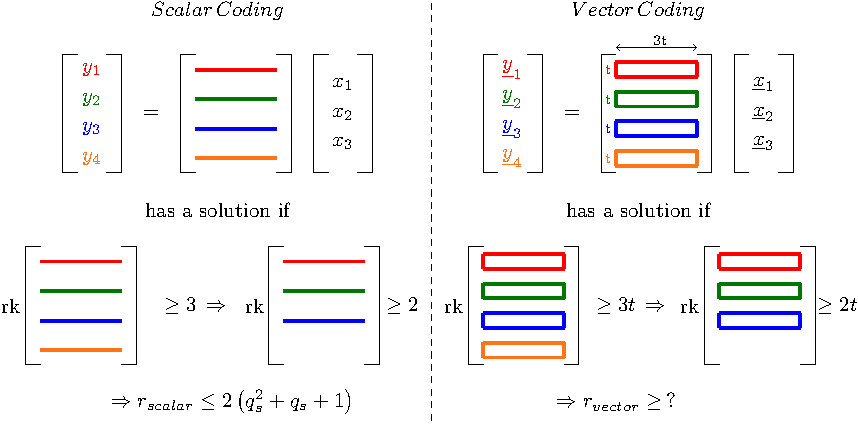
\includegraphics[width=0.6\paperwidth]{../figures/rk_h3}
\end{figure}

Following to (\ref{eq:linear_system}), each receiver $R_{j}$ has
to solve a linear equation system of $3t$ variables with $4t$ equations
to recover $h=3$ messages as below:
\begin{equation}
\left[\begin{array}{c}
\boldsymbol{y}_{j}^{\left(1\right)}\\
\boldsymbol{y}_{j}^{\left(2\right)}\\
\boldsymbol{y}_{j}^{\left(3\right)}\\
\boldsymbol{y}_{j}^{\left(4\right)}
\end{array}\right]=\boldsymbol{A}_{j}\cdot\underline{x}=\left[\begin{array}{c}
\boldsymbol{A}^{\left(r_{1}\right)}\\
\boldsymbol{A}^{\left(r_{2}\right)}\\
\boldsymbol{A}^{\left(r_{3}\right)}\\
\boldsymbol{B}^{\left(j\right)}
\end{array}\right]\cdot\left[\begin{array}{c}
\boldsymbol{x}_{1}\\
\boldsymbol{x}_{2}\\
\boldsymbol{x}_{3}
\end{array}\right],\label{eq:linear_system_h3rs4}
\end{equation}
with $\boldsymbol{x}_{1},\ldots,\boldsymbol{x}_{3}\in\ensuremath{\mathbb{F}}_{q}^{t},\boldsymbol{y}_{j}^{\left(1\right)},\ldots,\boldsymbol{y}_{j}^{\left(4\right)}\in\ensuremath{\mathbb{F}}_{q}^{t},\boldsymbol{A}^{\left(r_{v}\right)},\in\ensuremath{\mathbb{F}}_{q}^{t\times3t}$
for $v=1,\ldots,3$ and $1\leq r_{1}<r_{2}<r_{3}\leq r$, and $\boldsymbol{B}^{\left(j\right)}\in\ensuremath{\mathbb{F}}_{q}^{t\times3t}$
for $j\in\left\{ 1,\ldots,\left(\begin{array}{c}
r\\
3
\end{array}\right)\right\} $.

The network is solvable, if $\boldsymbol{A}_{j}$ has full rank as
following,
\[
\mathrm{rk}\left[\begin{array}{c}
\boldsymbol{A}^{\left(r_{1}\right)}\\
\boldsymbol{A}^{\left(r_{2}\right)}\\
\boldsymbol{A}^{\left(r_{3}\right)}\\
\boldsymbol{B}^{\left(j\right)}
\end{array}\right]\geq3t.
\]

Since coding coefficients for $\boldsymbol{B}^{\left(j\right)}$ can
be independently chosen for any receiver $R_{j}$, there always exists
$\boldsymbol{B}^{\left(j\right)}$ such that
\begin{equation}
\mathrm{rk}\left[\begin{array}{c}
\boldsymbol{A}^{\left(r_{1}\right)}\\
\boldsymbol{A}^{\left(r_{2}\right)}\\
\boldsymbol{A}^{\left(r_{3}\right)}
\end{array}\right]\geq2t,\label{eq:rk_rqm_e1l1h3s4}
\end{equation}
if and only if $\mathrm{rk}\left[\boldsymbol{A}_{j}\right]\geq3t$.

We formalize the problem by an approach with Lov\'asz local lemma,
which was initially proposed by Schwartz in \cite{MosheSchwartz:2018}.

Let $\mathcal{E}_{r_{1},r_{2},r_{3}}$ be an event that a receiver
$R_{j}$ is assigned a transfer matrix $\boldsymbol{A}_{j}$ such
that $\mathrm{rk}\left[\begin{array}{c}
\boldsymbol{A}^{\left(r_{1}\right)}\\
\boldsymbol{A}^{\left(r_{2}\right)}\\
\boldsymbol{A}^{\left(r_{3}\right)}
\end{array}\right]<2t$, i.e.,

\[
\mathcal{E}_{r_{1},r_{2},r_{3}}=\left\{ \mathrm{rk}\left[\begin{array}{c}
\boldsymbol{A}^{\left(r_{1}\right)}\\
\boldsymbol{A}^{\left(r_{2}\right)}\\
\boldsymbol{A}^{\left(r_{3}\right)}
\end{array}\right]<2t\right\} ,
\]

for $1\leq r_{1}<r_{2}<r_{3}\leq r$ and $\boldsymbol{A}^{\left(r_{1}\right)},\ldots,\boldsymbol{A}^{\left(r_{3}\right)}\in\ensuremath{\mathbb{F}}_{q}^{t\times3t}$,
chosen idenpendently and uniformly random.
\begin{lem}[Symmetric Lov\'asz local lemma (LLL) \cite{Schwarz:2013}]
 A set of events $\mathcal{E}_{i}$, such that each event occurs
with probability at most $p$. If each event is independent of all
others except for at most $d$ of them and $4pd\leq1$, then: $\mathrm{Pr}\left[\stackrel[i=1]{n}{\bigcap}\overline{\mathcal{E}}_{i}\right]>0$.
\label{thm:LLL}
\end{lem}
In \cite{Overbeck:2007}, the number of $\left[n\times m\right]$
matrices of rank $i$ over $\ensuremath{\mathbb{F}}_{q}$ is given,

\begin{equation}
\mathrm{NM}_{i,n,m}=\stackrel[j=0]{i-1}{\mathop{\prod}}\frac{\left(q^{m}-q^{j}\right)\left(q^{n}-q^{j}\right)}{q^{i}-q^{j}}.\label{eq:num_of_rank_t_matrices}
\end{equation}

We therefore have $\mathrm{NM}_{i<2t,3t,3t}$ as the number of $\left[3t\times3t\right]$
matrices whose ranks are less than $2t$. Each event $\mathcal{E}_{r_{1},r_{2},r_{3}}$
has a probability calculated by dividing $\mathrm{NM}_{i<2t,3t,3t}$
by $q^{9t^{2}}$, where $q^{9t^{2}}$ is the number of all possible
$\left[3t\times3t\right]$ matrices over $\ensuremath{\mathbb{F}}_{q}$.
The probability is bounded as stated in Lemma \ref{lem:prob_p_LLL_formula}
and we now apply the LLL for events $\mathcal{E}_{r_{1},r_{2},r_{3}}$.
\begin{lem}
\label{lem:prob_p_LLL_formula} $\mathrm{Pr}\left[\mathcal{E}_{r_{1},r_{2},r_{3}}\right]=p\in\Theta\left(q^{-t^{2}-2t-1}\right),\forall t\geq2.$
\end{lem}
\begin{proof}
Following to (\ref{eq:rk_rqm_e1l1h3s4}), a event $\mathcal{E}_{r_{1},r_{2},r_{3}}$
occurs when $\mathrm{rk}\left[\boldsymbol{A}_{j}\right]<3t$, and
its probability is bounded by $p$ (with $0\leq p\leq1$) as following,
\begin{eqnarray}
\mathrm{Pr}\left[\mathcal{E}_{r_{1},r_{2},r_{3}}\right]=\mathrm{Pr}\left[\mathrm{rk}\left[\begin{array}{c}
\boldsymbol{A}^{\left(r_{1}\right)}\\
\boldsymbol{A}^{\left(r_{2}\right)}\\
\boldsymbol{A}^{\left(r_{3}\right)}
\end{array}\right]<2t\right] & = & \stackrel[i=0]{2t-1}{\mathop{\sum}}\mathrm{Pr}\left[\mathrm{rk}\left[\begin{array}{c}
\boldsymbol{A}^{\left(r_{1}\right)}\\
\boldsymbol{A}^{\left(r_{2}\right)}\\
\boldsymbol{A}^{\left(r_{3}\right)}
\end{array}\right]=i\right]\label{eq:p_in_LLL}\\
 & \overset{1}{=} & \stackrel[i=0]{2t-1}{\mathop{\sum}}\frac{\mathrm{NM}_{i,3t,3t}}{q^{\left(3t\right)\cdot\left(3t\right)}}\nonumber \\
 & = & \stackrel[i=0]{2t-1}{\mathop{\sum}}\frac{\stackrel[j=0]{i-1}{\mathop{\prod}}\frac{\left(q^{3t}-q^{j}\right)^{2}}{q^{i}-q^{j}}}{q^{9t^{2}}}.\label{eq:p_eq_h3}
\end{eqnarray}

(1): Applying (\ref{eq:num_of_rank_t_matrices}) for $\left[3t\times3t\right]$
matrices over $\ensuremath{\mathbb{F}}_{q}$ of rank $i=0,\ldots,2t-1$.

In the following, we view $\stackrel[j=0]{i-1}{\mathop{\prod}}\frac{\left(q^{3t}-q^{j}\right)^{2}}{q^{i}-q^{j}}$
as a polynomial in $q$.

We consider the numerator of (\ref{eq:p_eq_h3}): $\stackrel[j=0]{i-1}{\mathop{\prod}}\frac{\left(q^{3t}-q^{j}\right)^{2}}{q^{i}-q^{j}}=\frac{p_{N}^{(i)}(q)}{p_{D}^{(i)}(q)}=p^{(i)}(q)$.

Due to $i$-times product and large $t$: $\left.\begin{array}{c}
\mathrm{deg}\left(p_{N}^{(i)}(q)\right)=q^{i6t}\\
\mathrm{deg}\left(p_{D}^{(i)}(q)\right)=q^{i^{2}}
\end{array}\right\} \Rightarrow p^{(i)}(q)\approx q^{i6t-i^{2}}$.

Therefore, we have: $\stackrel[i=0]{2t-1}{\mathop{\sum}}\stackrel[j=0]{i-1}{\mathop{\prod}}\frac{\left(q^{3t}-q^{j}\right)^{2}}{q^{i}-q^{j}}=\stackrel[i=0]{2t-1}{\mathop{\sum}}p^{(i)}(q)\approx\stackrel[i=0]{2t-1}{\mathop{\sum}}q^{i6t-i^{2}}$.

To maximize the sum, we set derivation of it to 0 and find the corresponding
root: 
\begin{eqnarray*}
 & \left(i6t-i^{2}\right)^{'} & =0\\
\Leftrightarrow & 6t-2i & =0\\
\Leftrightarrow & i & =3t.
\end{eqnarray*}

However, the upper limit of the sum is $\left(2t-1\right)$, which
is less than $3t$ for all $t\geq2$.
\[
\Rightarrow\mathrm{max}\left\{ q^{i6t-i^{2}}:i=0,2\ldots,2t-1\right\} =\left.q^{i6t-i^{2}}\right|_{i=2t-1}=q^{8t^{2}-2t-1}.
\]

Hence,
\[
\underset{i}{\mathrm{max}}\left\{ \stackrel[i=0]{2t-1}{\mathop{\sum}}p^{(i)}(q)\right\} \in\Theta\left(\mathrm{max}\left\{ q^{i6t-i^{2}}:i=1,2\ldots,2t-1\right\} \right)=\Theta\left(q^{8t^{2}-2t-1}\right)
\]
\[
\Rightarrow\underset{i}{\mathrm{max}}\left\{ \frac{\stackrel[i=0]{2t-1}{\mathop{\sum}}p^{(i)}(q)}{q^{9t^{2}}}\right\} \in\Theta\left(q^{-t^{2}-2t-1}\right)
\]
\[
\Rightarrow p\in\Theta\left(q^{-t^{2}-2t-1}\right)
\]
\end{proof}
Each event considered under the Lov\'asz Local Lemma \ref{thm:LLL}
is not required to be independent to all other events, and it allows
some dependence among events stated in Lemma \ref{lem:dependecy_d_LLL}.
\begin{lem}
Each event $\mathcal{E}_{r_{1},r_{2},r_{3}}$ is dependent on at most
$d\left(r\right)\leq\frac{3}{2}r^{2}$ other events. \label{lem:dependecy_d_LLL}
\end{lem}
\begin{proof}
It is clear that $\mathcal{E}_{r_{1},r_{2},r_{3}}$ is dependent on
$\mathcal{E}_{r_{1}^{'},r_{2}^{'},r_{3}^{'}}$ if and only if $\left\{ r_{1},r_{2},r_{3}\right\} \cap\left\{ r_{1}^{'},r_{2}^{'},r_{3}^{'}\right\} \neq\emptyset$.
Let us consider $\left\{ r_{1},r_{2},r_{3}\right\} \cap\left\{ r_{1}^{'},r_{2}^{'},r_{3}^{'}\right\} =\left\{ r_{1}\right\} =\left\{ r_{1}^{'}\right\} $,
we have maximum $\left(\begin{array}{c}
r-1\\
2
\end{array}\right)$ such $\mathcal{E}_{r_{1},r_{2},r_{3}}$ events. Similarly with $\left\{ r_{1},r_{2},r_{3}\right\} \cap\left\{ r_{1}^{'},r_{2}^{'},r_{3}^{'}\right\} =\left\{ r_{2}\right\} $
and $\left\{ r_{1},r_{2},r_{3}\right\} \cap\left\{ r_{1}^{'},r_{2}^{'},r_{3}^{'}\right\} =\left\{ r_{3}\right\} $,
we obtain
\[
d\left(r\right)\leq3\cdot\left(\begin{array}{c}
r-1\\
2
\end{array}\right)=3\cdot\frac{\left(r-1\right)\left(r-2\right)}{2}=\frac{3}{2}\left(r^{2}-3r+2\right)
\]
\[
\Rightarrow d\left(r\right)\leq\frac{3}{2}r^{2}
\]

Therefore, each event $\mathcal{E}_{r_{1},r_{2},r_{3}}$ is independent
of all other events except at most $d\leq\frac{3}{2}r^{2}$ of them.
\end{proof}
\begin{thm}
There is an $r_{\mathrm{max,vector}}\in\Omega\left(q^{t^{2}/2+\mathcal{O}\left(t\right)}\right)$
such that for any $r\leq r_{\mathrm{max,vector}}$ there exists a
vector solution for the $\left(\epsilon=1,l=1\right)-\mathcal{N}_{h=3,r,s=4}$
network . \label{theo:r_for_vector_sol_e1l1h3rs4}
\end{thm}
\begin{proof}
By the intersection rule, none of the $\mathcal{E}_{r_{1},r_{2},r_{3}}$
events occuring is equivalent to an event $T$ whose set of outcomes
satisfy (\ref{eq:rk_rqm_e1l1h3s4}) as following,
\[
T=\stackrel[i=1]{n}{\bigcap}\overline{\mathcal{E}}_{i}=\left\{ \mathrm{rk}\left[\begin{array}{c}
\boldsymbol{A}^{\left(r_{1}\right)}\\
\boldsymbol{A}^{\left(r_{2}\right)}\\
\boldsymbol{A}^{\left(r_{3}\right)}
\end{array}\right]\geq2t,\forall1\leq r_{1}<r_{2}<r_{3}\leq r\right\} .
\]
The Lov\'asz Local Lemma \ref{thm:LLL} shows that $\mathrm{Pr}\left[T\right]=\mathrm{Pr}\left[\stackrel[i=1]{n}{\bigcap}\overline{\mathcal{E}}_{i}\right]>0$
if $4\cdot p\cdot d(r)\leq1,\forall r\leq r_{\mathrm{max,vector}}$.
Furthermore, we have $d\leq\frac{3}{2}r^{2}$ following to Lemma \ref{lem:dependecy_d_LLL},
which gives: $4\cdot p\cdot\frac{3}{2}r^{2}\leq1\Rightarrow r\leq\sqrt{\frac{1}{6p}}=r_{\mathrm{max,vector}}$.

By Lemma \ref{lem:prob_p_LLL_formula}, we have $p\in\Theta\left(q^{-t^{2}-2t-1}\right)$,
\[
\Rightarrow r_{\mathrm{max,vector}}\in\Omega\left(\sqrt{\frac{1}{6p}}\right)=\Omega\left(\sqrt{\frac{1}{6q^{-t^{2}-2t-1}}}\right)=\Omega\left(q^{t^{2}/2+\mathcal{O}\left(t\right)}\right).
\]
The sufficient condition of Lemma \ref{thm:LLL} is satisfied for
any $r\leq r_{\mathrm{max,vector}}\in\Omega\left(q^{t^{2}/2+\mathcal{O}\left(t\right)}\right)$.
None of the $\mathcal{E}_{r_{1},r_{2},r_{3}}$ events occurs, so there
exists a vector solution for such $r$.
\end{proof}
\begin{cor}
The $\left(\epsilon=1,\ell=1\right)-\mathcal{N}_{h=3,r,s=4}$ network
has a vector solution with a gap $q^{t^{2}/4+\mathcal{O}(t)}$.
\end{cor}
\begin{proof}
In \cite[Sec. VIII-C]{Wachter-Zeh:2018}, we have that $r_{\mathrm{max,scalar}}\in\mathcal{O}\left(q_{\mathrm{s}}^{2}\right)$,
where they proved that
\begin{equation}
r_{\mathrm{scalar}}\leq2\left[\begin{array}{c}
3\\
1
\end{array}\right]_{q_{\mathrm{s}}}=2\left(q_{\mathrm{s}}^{2}+q_{\mathrm{s}}+1\right).\label{eq:r_scalar_max}
\end{equation}
Following to Section \ref{subsec:Comparison-between-scalar-and-vector-sol}
and Theorem \ref{theo:r_for_vector_sol_e1l1h3rs4}, we have the gap
size 
\begin{eqnarray}
 & r_{\mathrm{max,scalar}} & =r_{\mathrm{max,vector}}\nonumber \\
\Leftrightarrow & q_{\mathrm{s,min,from\,bound}}^{2} & =q^{t^{2}/2+\mathcal{O}(t)}\nonumber \\
\Leftrightarrow & q_{\mathrm{s,min,from\,bound}} & ^{=}q^{t^{2}/4+\mathcal{O}(t)}\nonumber \\
\Rightarrow & g_{\mathrm{lower\,bound}} & =q_{\mathrm{s,min,from\,bound}}-q_{v}=q^{t^{2}/4+\mathcal{O}(t)}\label{eq:gap_e1l1h3rs4}
\end{eqnarray}

Therefore, there exists a vector solution for the network to achieve
such gap.
\end{proof}
\begin{table}[H]
\begin{centering}
\begin{tabular}{|c|c|c|}
\hline 
t & Scalar Solution & Vector Solution\tabularnewline
\hline 
\hline 
2 & $r_{\mathrm{max,scalar}}=42$ & $r_{\mathrm{max,vector}}\geq7$\tabularnewline
\hline 
3 & $r_{\mathrm{max,scalar}}=146$ & $r_{\mathrm{max,vector}}\geq62$ \tabularnewline
\hline 
4 & $r_{\mathrm{max,scalar}}=546$ & $r_{\mathrm{max,vector}}\geq1317$\tabularnewline
\hline 
5 & $r_{\mathrm{max,scalar}}=2114$ & $r_{\mathrm{max,vector}}\geq58472$\tabularnewline
\hline 
6 & $r_{\mathrm{max,scalar}}=8322$ & $r_{\mathrm{max,vector}}>10^{6}$\tabularnewline
\hline 
\end{tabular}
\par\end{centering}
\centering{}\caption{Number of intermediate nodes $r$ for the $\left(\epsilon=1,\ell=1\right)-\mathcal{N}_{h=3,r,s=4}$
network such that scalar and vector solutions exist over $t=2,\ldots,6$.
Following to (\ref{eq:r_scalar_max}), there exists a scalar solution
for the network if and only if $r\protect\leq2\left(q_{s}^{2}+q_{s}+1\right)=r_{\mathrm{max,scalar}}$.
Following to (\ref{eq:p_eq_h3}) and Lemma \ref{lem:dependecy_d_LLL},
we observed that vector solutions outperforming the scalar solution
when $t\protect\geq4$. \label{tab:r_over_t}}
\end{table}

By varying $t$ in (\ref{eq:p_eq_h3}), we have the Table \ref{tab:r_over_t}.
In the Table \ref{tab:r_over_t}, the vector solution outperforms
the scalar solution when $t\geq4$ for the network $\left(\epsilon=1,\ell=1\right)-\ensuremath{N}_{h=3,r,s=4}$.
In Section \ref{sec:Main-Approach} and Section \ref{sec:Alternative-Approaches}
for computational results of the network, we show vector solutions
outperforming scalar solutions in case of $t=2$ and $t=3$.

\section{$\left(\epsilon=1,\ell=1\right)-\mathcal{N}_{h,r,s}$ Network \label{sec:e1l1_nw}}

The $\left(\epsilon=1,\ell=1\right)-\mathcal{N}_{h,r,s}$ network
is a more general network compared to the $\left(\epsilon=1,\ell=1\right)-\mathcal{N}_{3,r,4}$
network studied in the previous subsection. We study a gap between
scalar and vector solutions for the $\left(1,1\right)-\mathcal{N}_{h,r,s}$
network by deriving a lower bound on the maximum number of intermediate
nodes $r$. Following to (\ref{eq:linear_system}) and an extension
of (\ref{eq:linear_system_h3rs4}), each receiver $R_{j}$ has to
solve a linear equation of $ht$ variables with $st$ equations to
recover $h$ messages as following,

\[
\left[\begin{array}{c}
\boldsymbol{y}_{j}^{\left(1\right)}\\
\vdots\\
\boldsymbol{y}_{j}^{\left(\alpha\right)}\\
\boldsymbol{y}_{j}^{\left(\alpha+1\right)}
\end{array}\right]=\boldsymbol{A}_{j}\cdot\underline{x}=\left[\begin{array}{c}
\boldsymbol{A}^{\left(r_{1}\right)}\\
\vdots\\
\boldsymbol{A}^{\left(r_{\alpha}\right)}\\
\boldsymbol{B}^{\left(j\right)}
\end{array}\right]\cdot\left[\begin{array}{c}
\boldsymbol{x}_{1}\\
\vdots\\
\boldsymbol{x}_{h}
\end{array}\right],
\]

with $\boldsymbol{x}_{1},\ldots,\boldsymbol{x}_{h}\in\ensuremath{\mathbb{F}}_{q}^{t},\boldsymbol{y}_{j}^{\left(1\right)},\ldots,\boldsymbol{y}_{j}^{\left(\alpha+1\right)}\in\ensuremath{\mathbb{F}}_{q}^{t},\boldsymbol{A}^{\left(r_{1}\right)},\ldots,\boldsymbol{A}^{\left(r_{\alpha}\right)}\in\ensuremath{\mathbb{F}}_{q}^{t\times ht}$
for $1\leq r_{1}<\ldots<r_{\alpha}\leq r$, $\boldsymbol{B}^{\left(j\right)}\in\ensuremath{\mathbb{F}}_{q}^{t\times ht}$
for $j\in\left\{ 1,\ldots,\left(\begin{array}{c}
r\\
\alpha
\end{array}\right)\right\} $.

Since coding coefficients for $\boldsymbol{B}^{\left(j\right)}$ can
be independently chosen for any receiver $R_{j}$, there always exists
$\boldsymbol{B}^{\left(j\right)}$ such that the network is solvable
with 
\[
\mathrm{rk}\left[\begin{array}{c}
\boldsymbol{A}^{\left(r_{1}\right)}\\
\vdots\\
\boldsymbol{A}^{\left(r_{\alpha}\right)}
\end{array}\right]\geq ht-t,
\]

if and only if the transfer matrix $\boldsymbol{A}_{j}$ has full
rank.

Similar to $\left(1,1\right)-\ensuremath{N}_{3,r,4}$, we apply the
Lov\'asz Local Lemma \ref{thm:LLL} for the following $\mathcal{E}_{r_{1},\ldots,r_{h-\epsilon}}$
to study the gap between scalar and vector solutions for the $\left(1,1\right)-\mathcal{N}_{h,r,s}$
network.

Let $\mathcal{E}_{r_{1},\ldots,r_{\alpha}}$ be an event that a receiver
$R_{j}$ is assigned a transfer matrix $\boldsymbol{A}_{j}$ such
that $\mathrm{rk}\left[\begin{array}{c}
\boldsymbol{A}^{\left(r_{1}\right)}\\
\vdots\\
\boldsymbol{A}^{\left(r_{\alpha}\right)}
\end{array}\right]<(h-1)t$, i.e.,

\[
\mathcal{E}_{r_{1},\ldots,r_{\alpha}}=\left\{ \mathrm{rk}\left[\begin{array}{c}
\boldsymbol{A}^{\left(r_{1}\right)}\\
\vdots\\
\boldsymbol{A}^{\left(r_{\alpha}\right)}
\end{array}\right]<(h-1)t\right\} ,
\]

for $1\leq r_{1}<\ldots<r_{\alpha}\leq r$ and $\boldsymbol{A}^{\left(r_{1}\right)},\ldots,\boldsymbol{A}^{\left(r_{\alpha}\right)}\in\ensuremath{\mathbb{F}}_{q}^{t\times ht}$,
chosen independently and uniformly random.
\begin{lem}
\label{lem:p_e1l1}$\mathrm{Pr}\left[\mathcal{E}_{r_{1},\ldots,r_{\alpha}}\right]=p\in\Theta\left(q^{\left(h-\alpha\right)t^{2}+\mathcal{O}(t)}\right),\forall t\geq2.$
\end{lem}
\begin{proof}
The probability of an event $\mathcal{E}_{r_{1},\ldots,r_{\alpha}}$
can be calculated by 

\begin{eqnarray}
\mathrm{Pr}\left[\mathcal{E}_{r_{1},\ldots,r_{\alpha}}\right] & = & \stackrel[i=0]{(h-1)t-1}{\mathop{\sum}}\mathrm{Pr}\left[\mathrm{rk}\left[\begin{array}{c}
\boldsymbol{A}^{\left(r_{1}\right)}\\
\vdots\\
\boldsymbol{A}^{\left(r_{\alpha}\right)}
\end{array}\right]=i\right]\nonumber \\
 & \overset{1}{=} & \stackrel[i=0]{(h-1)t-1}{\mathop{\sum}}\frac{\mathrm{NM}_{i,\alpha t,ht}}{q^{\left(\alpha t\right)\left(ht\right)}}\nonumber \\
 & = & \frac{1}{q^{\left(\alpha h\right)t^{2}}}\cdot\stackrel[i=0]{(h-1)t-1}{\mathop{\sum}}\stackrel[j=0]{i-1}{\mathop{\prod}}\frac{\left(q^{\alpha t}-q^{j}\right)\left(q^{ht}-q^{j}\right)}{q^{i}-q^{j}}.\label{eq:general_nw_calc_p}
\end{eqnarray}

(1): The formula for the number of $\left[\alpha t\times ht\right]$
matrices of rank $i$ over $\ensuremath{\mathbb{F}}_{q}$ was introduced
in the previous subsection as (\ref{eq:num_of_rank_t_matrices}).

We consider firstly the product $\stackrel[j=0]{i-1}{\mathop{\prod}}\frac{\left(q^{\alpha t}-q^{j}\right)\left(q^{ht}-q^{j}\right)}{q^{i}-q^{j}}$
as a polynomial in $q$, then we have

\[
\stackrel[j=0]{i-1}{\mathop{\prod}}\frac{\left(q^{\alpha t}-q^{j}\right)\left(q^{ht}-q^{j}\right)}{q^{i}-q^{j}}=\frac{p_{N}^{(i)}(q)}{p_{D}^{(i)}(q)}=p^{(i)}(q).
\]

For $t\rightarrow\infty$: $\left.\begin{array}{c}
\mathrm{deg}\left(p_{N}^{(i)}(q)\right)=q^{i(\alpha t+ht)}\\
\mathrm{deg}\left(p_{D}^{(i)}(q)\right)=q^{i^{2}}
\end{array}\right\} \Rightarrow p^{(i)}(q)\approx q^{i(\alpha t+ht)-i^{2}}.$

Now, we evaluate the function $f(i)=i(\alpha t+ht)-i^{2}$ to find
its maximum point by its derivation, 

$f'(i^{*})=0\Leftrightarrow(\alpha t+ht)-2i^{*}=0\Leftrightarrow i^{*}=\frac{\alpha t+ht}{2}.$

Considering the sum $\stackrel[i=0]{(h-1)t-1}{\mathop{\sum}}p^{(i)}(q)$,
we have to check whether the point $i^{*}$ in $\left\{ 0,\ldots,(h-1)t-1\right\} $.
For the lower bound, we need $0\leq i^{*}\Leftrightarrow0\leq\frac{\alpha t+ht}{2}\Leftrightarrow t\geq\frac{2}{\alpha+h}$,
which is always true due to the given $t\geq2$ and $\alpha,h\geq3$
following to Theorem \ref{nw_parameters}.

Regarding to the upper bound, we need $\frac{\alpha t+ht}{2}\leq(h-1)t-1\Leftrightarrow t\leq\frac{-2}{\alpha+2-h}$.
Furthermore, we always have $\alpha+2>h$ due to $\alpha l+\epsilon=\alpha+1\geq h$
by Theorem \ref{nw_parameters}. Thus we need $t<0$ for $i^{*}\in\left\{ 0,\ldots,(h-1)t-1\right\} $,
which cannot happen since we always have $t\geq2$ for a vector solution.
For $i\in\left\{ 0,\ldots,(h-1)t-1\right\} $, the maximum value of
$q^{i(\alpha t+ht)-i^{2}}$ is therefore as following,
\begin{eqnarray*}
\mathrm{max}\left\{ q^{i(\alpha t+ht)-i^{2}}:i=0,\ldots,(h-1)t-1\right\}  & = & \left.q^{i(\alpha t+ht)-i^{2}}\right|_{i=(h-1)t-1}\\
 & = & q^{\left[\left(h-1\right)\left(\alpha+1\right)\right]t^{2}-\left(\alpha-h+2\right)t-1}.
\end{eqnarray*}

Secondly, we apply the maximum value to the sum, we have:
\begin{eqnarray*}
 & \mathrm{max}\left\{ \stackrel[i=0]{(h-1)t-1}{\mathop{\sum}}p^{(i)}(q)\right\}  & \in\Theta\left(q^{\left[\left(h-1\right)\left(\alpha+1\right)\right]t^{2}+\mathcal{O}(t)}\right)\\
\Rightarrow & \mathrm{max}\left\{ \frac{\stackrel[i=0]{(h-1)t-1}{\mathop{\sum}}p^{(i)}(q)}{q^{\left(\alpha h\right)t^{2}}}\right\}  & \in\Theta\left(\frac{q^{\left[\left(h-1\right)\left(\alpha+1\right)\right]t^{2}+\mathcal{O}(t)}}{q^{\left(\alpha h\right)t^{2}}}\right)
\end{eqnarray*}
\[
\Rightarrow p\in\Theta\left(q^{\left(h-\alpha-1\right)t^{2}+\mathcal{O}(t)}\right)
\]

Therefore, we have that each event $\mathcal{E}_{r_{1},\ldots,r_{\alpha}}$
 occurs with probability at most $p\in\Theta\left(q^{\left(h-\alpha-1\right)t^{2}+\mathcal{O}(t)}\right)$.
\end{proof}
\begin{lem}
Each event $\mathcal{E}_{r_{1},\ldots,r_{h-\epsilon}}$ is dependent
for at most $d\left(r\right)\leq\frac{\alpha}{\left(\alpha-1\right)!}r^{^{\alpha-1}}$
other events. \label{lem:d_e1l1}
\end{lem}
\begin{proof}
Similar to $\left(\epsilon=1,\ell=1\right)-\ensuremath{N}_{3,r,4}$,
we have:
\[
d\leq\alpha\left(\begin{array}{c}
r-1\\
\alpha-1
\end{array}\right)=\alpha\frac{\left(r-1\right)\ldots\left(r-\alpha+1\right)}{\left(\alpha-1\right)!}\leq\frac{\alpha}{\left(\alpha-1\right)!}r^{^{\alpha-1}}
\]
\end{proof}
\begin{thm}
There is $r_{\mathrm{max,vector}}\in\Omega\left(q^{\frac{h-\alpha-1}{1-\alpha}t^{2}+\mathcal{O}(t)}\right)$
such that for any $r\leq r_{\mathrm{max,vector}}$ there exists a
vector solution for the $\left(\epsilon=1,\ell=1\right)-\ensuremath{N}_{h,r,s}$
network. \label{theo:r_vector_e1l1}
\end{thm}
\begin{proof}
Following to the Lov\'asz Local Lemma \ref{thm:LLL} and Lemma \ref{lem:d_e1l1},
there exists a vector solution for the network if $4dp\leq1\Rightarrow d\leq\frac{\alpha}{\left(\alpha-1\right)!}r^{^{\alpha-1}}\Rightarrow r\leq\left(\frac{\left(\alpha-1\right)!}{4\alpha}\cdot\frac{1}{p}\right)^{\frac{1}{\alpha-1}}=r_{\mathrm{max,vector}}$.
By Lemma \ref{lem:d_e1l1}, we further have $p\in\Theta\left(q^{\left(h-\alpha-1\right)t^{2}+\mathcal{O}(t)}\right),\forall t\geq2$
as an upper bound of $\mathrm{Pr}\left[\mathcal{E}_{r_{1},\ldots,r_{\alpha}}\right]$.
Applying such $p$ to $r_{\mathrm{max,vector}}$, we therefore have
$r_{\mathrm{max,vector}}\in\Omega\left(q^{\frac{h-\alpha-1}{1-\alpha}t^{2}+\mathcal{O}(t)}\right)$.

Hence, the sufficient condition of the Local lemma \ref{thm:LLL}
is satisfied for any $r\leq r_{\mathrm{max,vector}}\in\Omega\left(q^{\frac{h-\alpha-1}{1-\alpha}t^{2}+\mathcal{O}(t)}\right)$
and a vector solution exists for such $r$.
\end{proof}
To calculate the gap, we then study scalar solutions for the $\left(1,1\right)-\ensuremath{N}_{h,r,s}$
network. Following to (\ref{eq:linear_system}) for a scalar solution,
each receiver $R_{j}$ have to solve the following linear system to
reconstruct its requested messages,

\[
\left[\begin{array}{c}
y_{j}^{\left(1\right)}\\
\vdots\\
y_{j}^{\left(\alpha\right)}\\
y_{j}^{\left(\alpha+1\right)}
\end{array}\right]=\left[\begin{array}{c}
\boldsymbol{a}^{\left(r_{1}\right)}\\
\vdots\\
\boldsymbol{a}^{\left(r_{\alpha}\right)}\\
\boldsymbol{b}^{\left(j\right)}
\end{array}\right]\cdot\left[\begin{array}{c}
x_{1}\\
\vdots\\
x_{h}
\end{array}\right],
\]

with $x_{1},\ldots,x_{h}\in\ensuremath{\mathbb{F}}_{q_{\mathrm{s}}},y_{j}^{\left(1\right)},\ldots,y_{j}^{\left(\alpha+1\right)}\in\ensuremath{\mathbb{F}}_{q_{\mathrm{s}}},\boldsymbol{a}^{\left(r_{1}\right)},\ldots,\boldsymbol{a}^{\left(r_{\alpha}\right)}\in\ensuremath{\mathbb{F}}_{q_{\mathrm{s}}}^{h}$
for $1\leq r_{1}<\ldots<r_{\alpha}\leq r$ and $\boldsymbol{b}^{\left(j\right)}\in\ensuremath{\mathbb{F}}_{q_{\mathrm{s}}}^{h}$
for $j\in\left\{ 1,\ldots,\left(\begin{array}{c}
r\\
\alpha
\end{array}\right)\right\} $. Similar to the vector solution studied for the $\left(1,1\right)-\ensuremath{N}_{h,r,s}$
network, there exists a scalar solution if

\begin{equation}
\mathrm{rk}\left[\begin{array}{c}
\boldsymbol{a}^{\left(r_{1}\right)}\\
\vdots\\
\boldsymbol{a}^{\left(r_{\alpha}\right)}
\end{array}\right]\geq h-1.\label{eq:rk_rqm_scalar_1_1_hrs}
\end{equation}

\begin{thm}
There exists $r_{\mathrm{max,scalar}}\in\mathcal{O}\left(q_{\mathrm{s}}^{\left(\alpha-h+2\right)\left(h-2\right)}\right)$
with $\alpha\geq h\geq3$ such that for any $r\leq r_{\mathrm{max,scalar}}$
there exists a scalar solution for the $\left(\epsilon=1,\ell=1\right)-\ensuremath{N}_{h,r,s}$
network. And there exists $r_{\mathrm{max,scalar}}\in\mathcal{O}\left(q_{\mathrm{s}}^{\alpha}\right)$
with $2\leq\alpha<h$ such that for any $r\leq r_{\mathrm{max,scalar}}$
there exists a scalar solution for the $\left(\epsilon=1,\ell=1\right)-\ensuremath{N}_{h,r,s}$
network. \label{theo:r_scalar_e1l1}
\end{thm}
\begin{proof}
Following to Theorem \ref{nw_parameters}, we are interested in network
parameters satisfying $\ell+\epsilon+1\leq h\leq\alpha\ell+\epsilon$.
Given $\epsilon=1,\ell=1$, we thus consider $\alpha$ and $h$ such
that $3\leq h\leq\alpha+1$, and we distinguish the following 2 cases.

For $2\leq\alpha<h$: since $h-1\leq\alpha<h$, we have then $\alpha=h-1$.
To satisfy $\mathrm{rk}\left[\begin{array}{c}
\boldsymbol{a}^{\left(r_{1}\right)}\\
\vdots\\
\boldsymbol{a}^{\left(r_{\alpha}\right)}
\end{array}\right]\geq h-1$, all $\boldsymbol{a}^{\left(r_{1}\right)},\ldots,\boldsymbol{a}^{\left(r_{\alpha}\right)}$
must be linearly independent. The number of intermediates nodes is
thus at most the number of distinct 1-dimensional subspaces of $\ensuremath{\mathbb{F}}_{q_{\mathrm{s}}}^{h}$and
therefore, a scalar solution exists if we have

\begin{eqnarray*}
 & r & \leq\left[\begin{array}{c}
h\\
1
\end{array}\right]_{q_{\mathrm{s}}}=\left[\begin{array}{c}
\alpha+1\\
1
\end{array}\right]_{q_{\mathrm{s}}}\\
\Rightarrow & r & \leq\frac{q_{\mathrm{s}}^{\alpha+1}-1}{q_{\mathrm{s}}-1}\approx q_{\mathrm{s}}^{\alpha}\\
\Rightarrow & r_{\mathrm{max,scalar}} & \in\mathcal{O}\left(q_{\mathrm{s}}^{\alpha}\right).
\end{eqnarray*}

For $\alpha\geq h\geq3$: to ensure that each receiver receives $\alpha$
vectors $\boldsymbol{a}^{\left(r_{1}\right)},\ldots,\boldsymbol{a}^{\left(r_{\alpha}\right)}\in\ensuremath{\mathbb{F}}_{q_{\mathrm{s}}}^{h}$
which span a subspace of $\ensuremath{\mathbb{F}}_{q_{\mathrm{s}}}^{h}$
whose dimension is at least $\left(h-1\right)$, i.e. a $\mathrm{(h-1)}$-subspace
of $\ensuremath{\mathbb{F}}_{q_{\mathrm{s}}}^{h}$, we have to guarantee
that on the links between the source and the intermediate nodes, no
$\alpha$ links will contain a vector which is contained in the same
$(h-2)$-subspace ($\left(\alpha-1\right)$ such links can have such
vectors). Hence, a scalar solution exists for this case if
\begin{eqnarray*}
 & r & \leq\left(\alpha-1\right)\left[\begin{array}{c}
\alpha\\
h-2
\end{array}\right]_{q_{\mathrm{s}}}\\
\Rightarrow & r & \leq\left(\alpha-1\right)\stackrel[i=0]{h-3}{\prod}\frac{q_{\mathrm{s}}^{\alpha}-q_{\mathrm{s}}^{i}}{q_{\mathrm{s}}^{h-2}-q_{\mathrm{s}}^{i}}\approx\left(\alpha-1\right)\left(q_{\mathrm{s}}^{\left(\alpha-h+2\right)\left(h-2\right)}\right)\\
\Rightarrow & r_{\mathrm{max,scalar}} & \in\mathcal{O}\left(q_{\mathrm{s}}^{\left(\alpha-h+2\right)\left(h-2\right)}\right).
\end{eqnarray*}

Therefore, with $2\leq\alpha<h$, there exists a scalar solution for
any $r\leq r_{\mathrm{max,scalar}}\in\mathcal{O}\left(q_{\mathrm{s}}^{\alpha}\right)$
and with $\alpha\geq h\geq3$, there exists a scalar solution for
any $r\leq r_{\mathrm{max,scalar}}\in\mathcal{O}\left(q_{\mathrm{s}}^{\left(\alpha-h+2\right)\left(h-2\right)}\right)$.
\end{proof}
Following to Theorem \ref{theo:r_vector_e1l1} and Theorem \ref{theo:r_scalar_e1l1},
we compute a gap for the network in Corollary \ref{cor:gap_e1l1}.
\begin{cor}
The $\left(\epsilon=1,\ell=1\right)-\ensuremath{N}_{h,r,s}$ network
has a vector solution with a gap $q^{\frac{\alpha-h+1}{\left(\alpha-1\right)\left(\alpha-h+2\right)\left(h-2\right)}t^{2}+\mathcal{O}(t)}$.
\label{cor:gap_e1l1}
\end{cor}
\begin{proof}
Following to Section \ref{subsec:Comparison-between-scalar-and-vector-sol},

\begin{eqnarray*}
 & r_{\mathrm{max,scalar}} & =r_{\mathrm{max,vector}}\\
\Leftrightarrow & q_{\mathrm{s,min,from\,bound}}^{\left(\alpha-h+2\right)\left(h-2\right)} & =q^{\frac{h-\alpha-1}{1-\alpha}t^{2}+\mathcal{O}(t)}\\
\Leftrightarrow & q_{\mathrm{s,min,from\,bound}} & ^{=}q^{\frac{\alpha-h+1}{\left(\alpha-1\right)\left(\alpha-h+2\right)\left(h-2\right)}t^{2}+\mathcal{O}(t)}\\
\Rightarrow & g_{\mathrm{lower\,bound}} & =q_{\mathrm{s,min,from\,bound}}-q_{v}=q^{\frac{\alpha-h+1}{\left(\alpha-1\right)\left(\alpha-h+2\right)\left(h-2\right)}t^{2}+\mathcal{O}(t)}
\end{eqnarray*}

Therefore, there exists a vector solution for the network to achieve
such gap.
\end{proof}
In the next subsection, we further study the gap for a more general
network compared to the $\left(1,1\right)-\ensuremath{N}_{h,r,s}$
network.

\section{$\left(\epsilon>1,\ell=1\right)-\mathcal{N}_{h,r,s}$ Network}

Due to the similarity of the $\left(1,1\right)-\ensuremath{N}_{h,r,s}$
networks, proofs can be found in Appendix \ref{app:proofs_e2l1}.
\begin{thm}
There is $r_{\mathrm{max,vector}}\in\Omega\left(q^{\frac{\epsilon\left(h-\alpha-\epsilon\right)}{1-\alpha}t^{2}+\mathcal{O}(t)}\right)$
such that for any $r\leq r_{\mathrm{max,vector}}$ there exists a
vector solution for the $\left(\epsilon>1,\ell=1\right)-\mathcal{N}_{h,r,s}$
network. \label{theo:e2l1_r_max_vector}
\end{thm}
%
\begin{thm}
There exists $r_{\mathrm{max,scalar}}\in\mathcal{O}\left(q_{\mathrm{s}}^{\left(\alpha-h+\epsilon+1\right)\left(h-\epsilon-1\right)}\right)$
with $\alpha\geq h\geq3$ such that for any $r\leq r_{\mathrm{max,scalar}}$
there exists a scalar solution for the $\left(\epsilon>1,\ell=1\right)-\mathcal{N}_{h,r,s}$
network. \label{theo:e2l1_r_max_scalar}
\end{thm}
Based on Theorem \ref{theo:e2l1_r_max_vector} and Theorem \ref{theo:e2l1_r_max_scalar},
we can then compute a gap between vector solutions and scalar solution
as mentioned in Corollary \ref{cor:e2l1_gap}.
\begin{cor}
The $\left(\epsilon>1,\ell=1\right)-\mathcal{N}_{h,r,s}$ network
has a vector solution with a gap $q^{\frac{\epsilon\left(\alpha-h+\epsilon\right)}{\left(\alpha-1\right)\left(\alpha-h+\epsilon+1\right)\left(h-\epsilon-1\right)}t^{2}+\mathcal{O}(t)}$.
\label{cor:e2l1_gap}
\end{cor}

\section{$\left(\epsilon=1,\ell>1\right)-\mathcal{N}_{h=2\ell,r,s=2\ell+1}$
Network}

Let $\mathcal{E}_{r_{1},\ldots,r_{h-\epsilon}}$ be an event that
a receiver $R_{j}$ is assigned a transfer matrix $\boldsymbol{A}_{j}$
such that $\mathrm{rk}\left[\begin{array}{c}
\boldsymbol{A}^{\left(r_{1}\right)}\\
\vdots\\
\boldsymbol{A}^{\left(r_{h-\epsilon}\right)}
\end{array}\right]<(2\ell-1)t$, i.e.,

\[
\mathcal{E}_{r_{1},\ldots,r_{\alpha}}=\left\{ \mathrm{rk}\left[\begin{array}{c}
\boldsymbol{A}^{\left(r_{1}\right)}\\
\vdots\\
\boldsymbol{A}^{\left(r_{h-\epsilon}\right)}
\end{array}\right]<\left(2\ell-1\right)t\right\} ,
\]

for $1\leq r_{1}<\ldots<r_{h-\epsilon}\leq r$ and $\boldsymbol{A}^{\left(r_{1}\right)},\ldots,\boldsymbol{A}^{\left(r_{h-\epsilon}\right)}\in\ensuremath{\mathbb{F}}_{q}^{t\times ht}$,
chosen independently and uniformly random.

We then apply the Lov\'asz Local Lemma \ref{thm:LLL} for events
.
\begin{lem}
\label{lem:p_e1l2} $\mathrm{Pr}\left[\mathcal{E}_{r_{1},\ldots,r_{h-\epsilon}}\right]\leq p\in\Theta\left(q^{-t^{2}-2t-1}\right),\forall t\geq2.$
\end{lem}
\begin{proof}
An event $\mathcal{E}_{r_{1},\ldots,r_{h-\epsilon}}$ has the following
probability:
\begin{eqnarray}
\mathrm{Pr}\left[\mathcal{E}_{r_{1},\ldots,r_{h-\epsilon}}\right] & = & \stackrel[i=0]{\left(2\ell-1\right)t-1}{\mathop{\sum}}\mathrm{Pr}\left[\mathrm{rk}\left[\begin{array}{c}
\boldsymbol{A}^{\left(r_{1}\right)}\\
\vdots\\
\boldsymbol{A}^{\left(r_{h-\epsilon}\right)}
\end{array}\right]=i\right]\nonumber \\
 & \overset{1}{=} & \stackrel[i=0]{\left(2\ell-1\right)t-1}{\mathop{\sum}}\frac{\mathrm{NM}_{i,2\ell t,2\ell t}}{q^{m\cdot n}}\nonumber \\
 & \overset{2}{=} & \frac{1}{q^{4\ell^{2}t^{2}}}\stackrel[i=0]{\left(2\ell-1\right)t-1}{\mathop{\sum}}\stackrel[j=0]{i-1}{\mathop{\prod}}\frac{\left(q^{2\ell t}-q^{j}\right)^{2}}{q^{i}-q^{j}}\label{eq:p_product_e1l2}
\end{eqnarray}

(1): The formula for the number of $\left[m\times n\right]$ matrices
of rank $i$ over $\ensuremath{\mathbb{F}}_{q}$ was proved in \cite{Overbeck:2007}
and was mentioned in (\ref{eq:num_of_rank_t_matrices}).

(2): $s=\alpha\ell+\epsilon$ by definition in Section \ref{sec:Description_GCN}
$\Rightarrow\alpha=2$, so $\boldsymbol{A}_{j}\in\ensuremath{\mathbb{F}}_{q}^{2\ell t\times2\ell t}$
with $\boldsymbol{A}_{j}=\left[\begin{array}{c}
\boldsymbol{A}^{\left(r_{1}\right)}\\
\vdots\\
\boldsymbol{A}^{\left(r_{h-\epsilon}\right)}
\end{array}\right]$, and $\boldsymbol{A}_{j}$ contains$\left(2\ell\right)$ $t$-dimensional
subspaces of $\ensuremath{\mathbb{F}}_{q}^{2\ell t}$.

We consider the product in (\ref{eq:p_product_e1l2}): $\stackrel[j=0]{i-1}{\mathop{\prod}}\frac{\left(q^{2\ell t}-q^{j}\right)^{2}}{q^{i}-q^{j}}=\frac{p_{N}^{(i)}(q)}{p_{D}^{(i)}(q)}=p^{(i)}(q)$.

Due to $i$-times product and large $t$: $\left.\begin{array}{c}
\mathrm{deg}\left(p_{N}^{(i)}(q)\right)=q^{i4\ell t}\\
\mathrm{deg}\left(p_{D}^{(i)}(q)\right)=q^{i^{2}}
\end{array}\right\} \Rightarrow p^{(i)}(q)\approx q^{i4\ell t-i^{2}}$.

Therefore, we have: $\stackrel[i=0]{\left(2\ell-1\right)t-1}{\mathop{\sum}}\stackrel[j=0]{i-1}{\mathop{\prod}}\frac{\left(q^{2\ell t}-q^{j}\right)^{2}}{q^{i}-q^{j}}=\stackrel[i=0]{\left(2\ell-1\right)t-1}{\mathop{\sum}}p^{(i)}(q)\approx\stackrel[i=0]{\left(2\ell-1\right)t-1}{\mathop{\sum}}q^{i4\ell t-i^{2}}$.

To maximize the sum, we set derivation of it to 0 and find the corresponding
root: 
\begin{eqnarray*}
 & \left(i4\ell t-i^{2}\right)^{'} & =0\\
\Leftrightarrow & 4\ell t-2i & =0\\
\Leftrightarrow & i & =2\ell t
\end{eqnarray*}
However, the upper limit of the sum is $\left(2\ell-1\right)t-1$,
which is less than $2\ell t$ for all $t\geq2$.

\[
\Rightarrow\mathrm{max}\left\{ q^{i4\ell t-i^{2}}:i=0,2\ldots,\left(2\ell-1\right)t-1\right\} =\left.q^{i4\ell t-i^{2}}\right|_{i=\left(2\ell-1\right)t-1}=q^{4\ell^{2}t^{2}-t^{2}-2t-1}
\]
Hence, by using the exact bound $\Theta$, we have:
\[
\underset{i}{\mathrm{max}}\left\{ \stackrel[i=0]{\left(2\ell-1\right)t-1}{\mathop{\sum}}p^{(i)}(q)\right\} \in\Theta\left(q^{4\ell^{2}t^{2}-t^{2}-2t-1}\right)
\]
\[
\Rightarrow\underset{i}{\mathrm{max}}\left\{ \frac{1}{q^{4\ell^{2}t^{2}}}\stackrel[i=0]{\left(2\ell-1\right)t-1}{\mathop{\sum}}p^{(i)}(q)\right\} \in\Theta\left(q^{-t^{2}-2t-1}\right)
\]
\[
\Rightarrow p\in\Theta\left(q^{-t^{2}-2t-1}\right)
\]
\end{proof}
\begin{lem}
Each event $\mathcal{E}_{i}$ is independent of all others except
for at most $d\leq2r$ of them. \label{lem:d_e1l2}
\end{lem}
\begin{proof}
Similar to the previous subsections, we have: 
\[
d\leq\alpha\left(\begin{array}{c}
r-1\\
\alpha-1
\end{array}\right)=2\frac{\left(r-1\right)\ldots\left(r-1\right)}{1!}\leq2r
\]

Therefore, each event is dependent on at most $d\leq2r$ other events.
\end{proof}
\begin{thm}
There exists $r_{\mathrm{max,vector}}\in\Omega\left(q^{t^{2}+\mathcal{O}\left(t\right)}\right)$
such that for any $r\leq r_{\mathrm{max,vector}}$ there exists a
vector solution for the $\left(\epsilon=1,\ell>1\right)-\mathcal{N}_{h=2\ell,r,s=2\ell+1}$
network. \label{theo:r_for_e1l2}
\end{thm}
\begin{proof}
As previous, we need $4\cdot p\cdot d(r)\leq1,\forall r\leq r_{\mathrm{max,vector}}$
so that a vector solution exists. Following to Lemma \ref{lem:d_e1l2},
we have $d\leq2r\Rightarrow4\cdot p\cdot2r\leq1\Rightarrow r\leq\frac{1}{8p}$.
And we have $p\in\Theta\left(q^{-t^{2}-2t-1}\right),\forall t\geq2$
in Lemma \ref{lem:p_e1l2} to get lower bound on $r_{\mathrm{max,vector}}$.
Thus, $r_{\mathrm{max,vector}}\in\Omega\left(\frac{1}{8p}\right)=\Omega\left(q^{t^{2}+2t+1}\right)$.

Hence, the Local lemma in \ref{thm:LLL} is satisfied for any $r\leq r_{\mathrm{max,vector}}\in\Omega\left(q^{t^{2}/2+\mathcal{O}\left(t\right)}\right)$.
None of the events $\mathcal{E}_{r_{1},\ldots,r_{h-\epsilon}}$ occurs,
so there exists a vector solution for such $r$.
\end{proof}
\begin{lem}
A scalar solution for the $\left(\epsilon=1,\ell>1\right)-\mathcal{N}_{h=2\ell,r,s=2\ell+1}$
network exists, if and only if there exists a Grasmannian code $\mathcal{G}_{q}\left(h=2\ell,\ell\right)$
such that any $\alpha=2$ subspaces of the set span a subspace of
dimension at least $2\ell-1$. 
\end{lem}
\begin{proof}
Any 2 $\ell$-dimensional subspaces of $\ensuremath{\mathbb{F}}_{q_{s}}^{2\ell}$
are distinct, so any 2 subspaces of the $\mathcal{G}_{q}\left(2\ell,\ell\right)$
span a subspace of dimension at least $2\ell-1$. The number of intermediate
nodes is therefore at most the number of distinct $\ell$-dimensional
subspaces of $\ensuremath{\mathbb{F}}_{q_{s}}^{2\ell}$, and a scalar
solution exists if
\[
r\leq\left[\begin{array}{c}
2\ell\\
2\ell-2
\end{array}\right]_{q_{s}}\Rightarrow r_{\mathrm{max,scalar}}\in\mathcal{O}\left(q_{s}^{l}\right)
\]
\end{proof}
\begin{cor}
The $\left(\epsilon=1,\ell>1\right)-\mathcal{N}_{h=2\ell,r,s=2\ell+1}$
network has a vector solution with a gap $q^{t^{2}/4+\mathcal{O}(t)}$.
\label{cor:gap_e1l2}
\end{cor}
Following to Section \ref{subsec:Comparison-between-scalar-and-vector-sol}
and Theorem \ref{theo:r_for_e1l2}, we have the gap size 
\begin{eqnarray}
 & r_{\mathrm{max,scalar}} & =r_{\mathrm{max,vector}}\nonumber \\
\Leftrightarrow & q_{\mathrm{s,min,from\,bound}}^{\ell} & =q^{t^{2}/2+\mathcal{O}(t)}\nonumber \\
\Leftrightarrow & q_{\mathrm{s,min,from\,bound}} & ^{=}q^{t^{2}/2\ell+\mathcal{O}(t)}\nonumber \\
\Rightarrow & g_{\mathrm{lower\,bound}} & =q_{\mathrm{s,min,from\,bound}}-q_{v}=q^{t^{2}/2\ell+\mathcal{O}(t)}\label{eq:gap_e1l2}
\end{eqnarray}

This shows us that there exists a better vector solution by comparison
with the gap in \cite[Fig. 4]{Wachter-Zeh:2018}.

\part{Computational Results}

In Table \ref{tab:r_over_t}, our vector solutions are computed by
Algorithm \ref{alg:Increasing-Method} for the $\left(\epsilon=1,\ell=1\right)-\ensuremath{N}_{3,r,4}$
network regarding to $t=2$ and $t=3$, with $q_{v}=q^{t}$ as previous
sections. Both construction 1 and 2 provide better results than scalar
solutions. 

Construction 1: $\begin{array}{c|c}
\boldsymbol{I}_{t} & \boldsymbol{T}\end{array}$, with $\boldsymbol{T}\in\ensuremath{\mathbb{F}}_{q}^{t\times t\left(h-1\right)}$,
which is clearly explained in Section \ref{sec:Alternative-Approaches}.

Construction 2: $\boldsymbol{T}\in U\left(t,3t\right)$, which is
described in the following Section \ref{sec:Main-Approach}.

\section{Incremental Algorithm (IM) \label{sec:Main-Approach}}

Regarding to $t=2$, for a scalar network coding solution we need
a $3-\left(3,1,1\right)_{4}^{c}$ code ($q_{v}=2^{2}=4)$ by Theorem
\ref{theo:scalar_sol_exist}. The largest such code consists of the
21 one-dimensionall subspaces of $\ensuremath{\mathbb{F}}_{4}^{3}$,
each one is contained twice in the code. Therefore, the number of
nodes can be at most 42 for a scalar linear coding solution, while
for vector network coding 89 nodes can be used, i..e. $\mathcal{A}_{q=2}\left(n=6,k=4,\mathrm{t}=3;\lambda=2\right)\geq89$
following to Corollary \ref{cor:dual_subspaces}. This is a new lower
bound for $\mathcal{A}_{2}\left(6,4,3;2\right)$ compared to a code
with 51 codewords presented in \cite{Wachter-Zeh:2018}. The smallest
alphabet size for a scalar solution with 89 nodes exists is $q_{s}=8$.
By (\ref{eq:r_scalar_max}), there are 73 one-dimensional subspaces
of $\ensuremath{\mathbb{F}}_{8}^{3}$, and each one can be used twice
in the code; therefore, we have in total 146 possible codesword, but
only 89 codewords are required. In this case, the gap size $g=q_{s}-q_{v}=2^{3}-2^{2}=8-4=2^{2},$i.e.
we achieve a gap size $q^{t^{2}/2}$, which is better the asymptotic
behavior in (\ref{eq:gap_e1l1h3rs4}). 

Before introducing the algorithm used to generate such 89 codewords,
we have to state some definitions for a beter explanation. We denote
a matrix space of dimension $\left[n\times m\right]$ by $M(n,m)=\left\{ \boldsymbol{A}:\boldsymbol{A}\in\ensuremath{\mathbb{F}}_{q=2}^{n\times m}\right\} $.
\begin{defn}[Matrix Space with Unique Row Space\label{def:urs_matrix_space}]
 $U(n,m)$ is a subset of $M(n,m)$, where any $\boldsymbol{A},\boldsymbol{B}\in U(n,m)$
have their row spaces such that:
\[
\mathcal{R}_{q}\left(\boldsymbol{A}\right)\neq\mathcal{R}_{q}\left(\boldsymbol{B}\right),
\]
where $\mathcal{R}_{q}\left(.\right)$ denotes the row space of a
matrix.
\end{defn}
%
\begin{defn}[Sufficient Global Coding Vector\label{def:sufficient_global_coding_vectors} ]
 Let $\boldsymbol{A},\boldsymbol{B},\boldsymbol{C}\in U(t,3t)$ and
$N\lll\left(\begin{array}{c}
2^{3t^{2}}\\
3
\end{array}\right)$, then a set $\mathcal{H}_{n=3t,m=3t}=\left\{ \boldsymbol{H}_{1},\ldots,\boldsymbol{H}_{N}\right\} $
contains distinct \textit{sufficient global coding vectors} $\boldsymbol{H}_{j}$
such that:
\[
\mathrm{rk}\left[\boldsymbol{H}_{j}\right]=\mathrm{rk}\left[\begin{array}{c}
\boldsymbol{A}\\
\boldsymbol{B}\\
\boldsymbol{C}
\end{array}\right]\geq2n,\forall j\in\left\{ 1,\ldots,N\right\} .
\]
For ease of notations, we denote $\left[\begin{array}{c}
\boldsymbol{A}\\
\boldsymbol{B}\\
\boldsymbol{C}
\end{array}\right]$ by $\left\{ \boldsymbol{A},\boldsymbol{B},\boldsymbol{C}\right\} $
for the rest of this thesis.
\end{defn}
%
\begin{defn}[Relative]
 Let $\boldsymbol{A},\boldsymbol{B},\boldsymbol{C}\in U(t,3t)$ introduced
in Definition \ref{def:urs_matrix_space}. Then $\boldsymbol{C}$
is called a \textit{relative} of a tuple $\left(\boldsymbol{A},\boldsymbol{B}\right)$
if $\left\{ \boldsymbol{A},\boldsymbol{B},\boldsymbol{C}\right\} \in\mathcal{H}_{n=3t,m=3t}$
and denoted as following:
\[
\mathrm{rel}\left[\left(\boldsymbol{A},\boldsymbol{B}\right)\right]=\boldsymbol{C}.
\]
\end{defn}
\begin{lem}
For any set $\mathcal{H}_{n=3t,m=3t}=\left\{ \boldsymbol{H}_{1},\ldots,\boldsymbol{H}_{N}\right\} $,
there are maximum $3\cdot\left(\begin{array}{c}
2^{3t^{2}}\\
3
\end{array}\right)$ relatives. \label{lem:num_of_relatives}
\end{lem}
\begin{proof}
Each sufficient global coding vector $\boldsymbol{H}_{j}$ contains
a $\left\{ \boldsymbol{A},\boldsymbol{B},\boldsymbol{C}\right\} $.
Thus, each of these 3 matrices can form 3 different relatives:
\[
\begin{array}{c}
\mathrm{rel}\left[\left(\boldsymbol{A},\boldsymbol{B}\right)\right]=\boldsymbol{C}\\
\mathrm{rel}\left[\left(\boldsymbol{A},\boldsymbol{C}\right)\right]=\boldsymbol{B}\\
\mathrm{rel}\left[\left(\boldsymbol{B},\boldsymbol{D}\right)\right]=\boldsymbol{A}
\end{array}.
\]
Furthermore, the maximum size of $\mathcal{H}_{n=3t,m=3t}$ introduced
in Defnition \ref{def:sufficient_global_coding_vectors} is $q^{3t^{2}}$.
Therefore, $\mathcal{H}_{t=3}$ can have only maximum $3q^{3t^{2}}$
relatives.
\end{proof}
\begin{defn}[Sub-relative]
 Let $\boldsymbol{A},\boldsymbol{B},\boldsymbol{C},\boldsymbol{D}\in U(t,3t)$.
Then $\boldsymbol{D}$ is called a \textit{sub-relative} of a tuple
$\left(\boldsymbol{A},\boldsymbol{B},\boldsymbol{C}\right)\in\mathcal{H}_{n=3t,m=3t}$
if:
\[
\left\{ \begin{array}{c}
\left\{ \boldsymbol{A},\boldsymbol{B},\boldsymbol{D}\right\} \in\mathcal{H}_{t=3}\\
\left\{ \boldsymbol{A},\boldsymbol{C},\boldsymbol{D}\right\} \in\mathcal{H}_{t=3}\\
\left\{ \boldsymbol{B},\boldsymbol{C},\boldsymbol{D}\right\} \in\mathcal{H}_{t=3}
\end{array}\right..
\]
A sub-relative is denoted by: 
\[
\mathrm{subrel}\left[\left(\boldsymbol{A},\boldsymbol{B},\boldsymbol{C}\right)\right]=\boldsymbol{D}.
\]
This definition about Sub-relative is similarly again used for a set
of 5 or more matrices.
\end{defn}
\begin{algorithm}[H]
\caption{Increasing Method \label{alg:Increasing-Method}}

\hspace*{\algorithmicindent} \textbf{Input}: $\mathcal{H}_{n=3t,m=3t}$ with its size $\left|\mathcal{H}_{n=3t,m=3t}\right|=N\lll\left(\begin{array}{c} 2^{3t^{2}}\\ 3 \end{array}\right)$. \\
\hspace*{\algorithmicindent} \textbf{Output}: A $3-\left(3t,t,t\right)_{q=2}^{c}$ code or its orthogonal complement, a $3-\left(3t,2t,t\right)_{q=2}^{m}$ with its code size is maximum under $\mathcal{H}_{n=3t,m=3t}$.  
\begin{algorithmic}[1]
	\FORALL{$\left(\textbf{A},\textbf{B},\textbf{C}\right) \in \mathcal{H}_{n=3t,m=3t}$}
    	\STATE {$R\leftarrow$ Generate all relatives; ({*})}
	\ENDFOR

	\STATE {$P_{\mathrm{max}}\leftarrow\{\}$ // an empty set}
	\FORALL{$\left(\textbf{X},\textbf{Y}\right) \in R$} 
		\IF{$\left|\mathrm{rel}\left[\left(\textbf{X},\textbf{Y}\right)\right]\right|$ is maximum}
			\STATE {$P_{\mathrm{max}}\leftarrow P_{\mathrm{max}}\oplus\left(\textbf{X},\textbf{Y}\right)$ ({**})} 
		\ENDIF
	\ENDFOR

	\STATE {$P_{potential}\leftarrow\{\}$ // an empty set}
	\FORALL{$\left(\textbf{E},\textbf{Q}\right) \in P_{max}$}
		\IF{$\left|\left(\textbf{E},\textbf{Q}\right)\cup rel\left[\left(\textbf{E},\textbf{Q}\right)\right]\right|\notin P_{potential}$}
			\STATE {$P_{\mathrm{potential}}\leftarrow P_{\mathrm{potential}}\oplus\left(\textbf{E},\textbf{Q}\right)$}
		\ENDIF
	\ENDFOR
	
	\STATE {$P\leftarrow\{\}$ // an empty set}
	\FORALL{$\left(\textbf{K},\textbf{L}\right) \in P_{\mathrm{potential}}$}
		\FORALL{$\textbf{Z} \in \mathrm{rel}\left[\left(\textbf{X},\textbf{Y}\right)\right]$}
			\IF{$\mathrm{subrel}\left[\left(\boldsymbol{K},\boldsymbol{L},\boldsymbol{Z}\right)\right]$ is maximum}
				\STATE {$P\leftarrow P_{\mathrm{potential}}\oplus\left(\textbf{K},\textbf{L},\textbf{Z}\right)$ ({***})}
			\ENDIF
		\ENDFOR 
	\ENDFOR
	
	\WHILE{$\exists \mathrm{subrel}$ in $P$ is not empty ({****})}
		\STATE {Line 10 to Line 23, but elements of $P_{\mathrm{max}}$ is replaced by $P$ and the size of subrel tuple is thus increased over each while loop.}
	\ENDWHILE
\end{algorithmic}
\end{algorithm}

({*}): If any 2-tuple exists already in $R$, its new relative is
appended to its existing relatives to form a set of relatives.

({*}{*}): $P_{max}$ is set to an empty set anytime we find a new
maximum, before the concatenation $\oplus$.

({*}{*}{*}): $P$ is set to an empty set anytime we find a new maximum,
before the concatenation $\oplus$. $P$ removes duplicated values
itself under the while-loop of Line 11 to Line 15.

({*}{*}{*}{*}): This means the maximum size of subrel in $P$ is not
0.

~

Now, we prove that Algorithm \ref{alg:Increasing-Method} always give
us our expected output. Then we compute its complexity based on number
of necessary computation.
\begin{thm}
Let $n=\left|U(t,3t)\right|$, then the Algorithm \ref{alg:Increasing-Method}
finds all matrices satisfying Equation \ref{eq:rk_rqm_e1l1h3s4} for
the $\left(1,1\right)-\ensuremath{N}_{3,r,4}$ network in $\mathcal{O}\left(n^{3}\right)$
operations.
\end{thm}
\begin{proof}
Our problem can be described by searching for a matrix subset $\boldsymbol{c}=\left[\boldsymbol{C}_{1},\ldots,\boldsymbol{C}_{w}\right]$
of the set $U(t,3t)$ over $\ensuremath{\mathbb{F}}_{2}^{t\times3t}$
with $w\leq n$, such that any 3 matrices in $\boldsymbol{c}$ satisfy
Equation \ref{eq:rk_rqm_e1l1h3s4}. 

Line 1 to Line 3 (\textit{Step 1}) of the algorithm is for the purpose
of generating all relatives of pairs of 2 matrices in $U(2,6)$. With
a large $n$, we have $3\cdot\left(\begin{array}{c}
n\\
3
\end{array}\right)\approx3n^{3}$ such pairs for generating relatives. Outputs of this step are in
the format of 
\[
\mathrm{rel}\left[\left(\boldsymbol{C}_{i},\boldsymbol{C}_{j}\right)\right],\forall\left(\boldsymbol{C}_{i},\boldsymbol{C}_{j}\right)\in\mathrm{Combination}\left(U(2,6),2\right),
\]
where $\mathrm{Combination}(S,k)$ gives us all k-tuples of elements
in $S$. Let us denote the size of each $\mathrm{rel}\left[\left(\boldsymbol{C}_{i},\boldsymbol{C}_{j}\right)\right]$
by $m$, and we achive $3n^{3}$ different sizes in a vector $\boldsymbol{m}=\left[m_{1},\ldots,m_{3n^{3}}\right].$
Step 1 therefore can be implemented in $\mathcal{O}\left(n^{3}\right)$
operations. Following to Theorem \ref{theo:size_rel}, $\mathrm{max}\left\{ \boldsymbol{m}\right\} $
is the upper bound for a code size, when $3-\left(3t,t,t\right)_{q=2}^{c}$
code for a vector solution is considered \cite[Sec. V-D]{Zhang:2019}.

Line 4 to Line 9 (\textit{Step 2}) is designed to find all pairs $\left(\boldsymbol{C}_{i},\boldsymbol{C}_{j}\right)$
whose $m=max\left\{ \boldsymbol{m}\right\} $. This step ensures that
our output of the algorithm generate the largest size for the subset
$\boldsymbol{c}$, which is equivalent to an optimal vector solution
regarding to the use of $3-\left(3t,t,t\right)_{q=2}^{c}$ code. Step
2 checks all elements in $\boldsymbol{m}$, and thus it can be computed
in $\mathcal{O}\left(n^{3}\right)$ operations.

Line 10 to Line 15 (\textit{Step 3}) is designed to keep only one
of above intial pairs $\left(\boldsymbol{C}_{i},\boldsymbol{C}_{j}\right)$
if its set $\left\{ \boldsymbol{C}_{i},\boldsymbol{C}_{j}\right\} \cup\mathrm{rel}\left[\left(\boldsymbol{C}_{i},\boldsymbol{C}_{j}\right)\right]$
is duplicated with any other such pairs. Step 3 can be implemented
in $\mathcal{O}\left(n^{3}\right)$ operations.

Line 16 to Line 23 (\textit{Step 4}) is for the purpose of extending
a next matrix for this pair to form sub-relatives $\mathrm{subrel}\left[\left(\boldsymbol{C}_{i},\boldsymbol{C}_{j},\boldsymbol{C}_{p}\right)\right]$
by checking all relatives of each pair $\left(\boldsymbol{C}_{i},\boldsymbol{C}_{j}\right)$
from Step 3. We have $\mathrm{max}\left\{ \boldsymbol{m}\right\} \leq n-2$
because such a pair can have maximum $n-2$ relatives. Step 4 thus
can be computed in $\mathcal{O}\left(n\right)$ operations.

Line 24 to Line 26 (\textit{Step 5}): if there exist a non-empty set
$\mathrm{subrel}\left[\left(\boldsymbol{C}_{i},\boldsymbol{C}_{j},\boldsymbol{C}_{p}\right)\right]$
from outputs of Step 4. We run a loop of Step 3 and Step 4. This first
loop checks maximum $n-3$ elements, because such a triplet can have
maximum $n-3$. It will linearly reduce over each loop, and each loop
is designed to generate sub-relative, which costs maximum $\mathcal{O}\left(n\right)$
operations. Therefore, step 5 can be implemented in $\mathcal{O}\left(n^{2}\right)$
operations.

Summarized, we obtain the complexity claimed in the theorem.
\end{proof}
We are going to list some toy examples for the algorithm as well as
illustrate it in Figure \ref{fig:rel_example}.
\begin{example}
Let $n=1,m=2,q=2$, which violates the input $\mathcal{H}_{n=3t,m=3t}$
but still being a good example for the rest steps in Algorithm \ref{alg:Increasing-Method}.
Then we have $N=4$ matrices (vectors):
\[
\begin{array}{c}
\boldsymbol{A}=[0,0]\\
\boldsymbol{B}=[0,1]\\
\boldsymbol{C}=[1,0]\\
\boldsymbol{D}=[1,1]
\end{array}
\]
\uline{Step 1} (Line 1 to Line 3): Due to, any 3 of them form a
sufficient global coding vector, i.e. a matrix whose rank is greater
than or equal to $2n$, we have the relative as following:
\[
\begin{array}{c}
\mathrm{rel}\left[\left(\boldsymbol{A},\boldsymbol{B}\right)\right]=[\boldsymbol{C},\boldsymbol{D}]\\
\mathrm{rel}\left[\left(\boldsymbol{A},\boldsymbol{C}\right)\right]=[\boldsymbol{B},\boldsymbol{D}]\\
\mathrm{rel}\left[\left(\boldsymbol{A},\boldsymbol{D}\right)\right]=[\boldsymbol{B},\boldsymbol{C}]\\
\mathrm{rel}\left[\left(\boldsymbol{B},\boldsymbol{C}\right)\right]=[\boldsymbol{A},\boldsymbol{D}]\\
\mathrm{rel}\left[\left(\boldsymbol{B},\boldsymbol{D}\right)\right]=[\boldsymbol{A},\boldsymbol{C}]\\
\mathrm{rel}\left[\left(\boldsymbol{C},\boldsymbol{D}\right)\right]=[\boldsymbol{A},\boldsymbol{B}]
\end{array}
\]
\uline{Step 2} (Line 4 to Line 9): We get the maximum size of these
steps is $2$ and $P_{max}$ results in all $\left\{ \boldsymbol{A},\boldsymbol{B}\right\} ,\left\{ \boldsymbol{A},\boldsymbol{C}\right\} ,\left\{ \boldsymbol{A},\boldsymbol{D}\right\} ,\left\{ \boldsymbol{B},\boldsymbol{C}\right\} ,\left\{ \boldsymbol{B},\boldsymbol{D}\right\} ,\left\{ \boldsymbol{C},\boldsymbol{D}\right\} $,
since 
\[
\underset{\begin{array}{c}
\forall\boldsymbol{X},\boldsymbol{Y}\in M(1,2)\\
\boldsymbol{X}\neq\boldsymbol{Y}
\end{array}}{\mathrm{max}}\left(\mathrm{rel}\left[\left(\boldsymbol{X},\boldsymbol{Y}\right)\right]\right)=2
\]
.

\uline{Step 3} (Line 10 to Line 14): Due to $\left\{ \boldsymbol{E},\boldsymbol{Q}\right\} \cup rel\left[\left(\boldsymbol{E},\boldsymbol{Q}\right)\right]=\left\{ \boldsymbol{A},\boldsymbol{B},\boldsymbol{C},\boldsymbol{D}\right\} $
with $\left(\boldsymbol{E},\boldsymbol{Q}\right)$ are tuples from
$P_{max}$ found in Step 2. We keep only $P_{\mathrm{potential}}=\left\{ \left(\boldsymbol{A},\boldsymbol{B}\right):\mathrm{rel}\left[\left(\boldsymbol{A},\boldsymbol{B}\right)\right]\right\} $

\uline{Step 4} (Line 16 to 23): Regarding to $\mathrm{rel}\left[\left(\boldsymbol{K},\boldsymbol{L}\right)\right]=\mathrm{rel}\left[\left(\boldsymbol{A},\boldsymbol{B}\right)\right]$,
we have $\boldsymbol{Z}\in\left\{ \boldsymbol{C},\boldsymbol{D}\right\} $.
Then, $\left|\mathrm{subrel}\left[\left(\boldsymbol{A},\boldsymbol{B},\boldsymbol{C}\right)\right]\right|=\left|\mathrm{subrel}\left[\left(\boldsymbol{A},\boldsymbol{B},\boldsymbol{D}\right)\right]\right|=1$,
so we get $P=\left\{ \left(\boldsymbol{A},\boldsymbol{B},\boldsymbol{C}\right),\left(\left(\boldsymbol{A},\boldsymbol{B},\boldsymbol{D}\right)\right)\right\} $.

\uline{Step 5}: The maximum size of subrel in $P$ is larger than
$0$, so we proceed the while loop. Step 3 will be looped firstly,
and we get $P_{\mathrm{potential}}=\left\{ \left(\boldsymbol{A},\boldsymbol{B},\boldsymbol{C}\right):\mathrm{rel}\left[\left(\boldsymbol{A},\boldsymbol{B},\boldsymbol{C}\right)\right]\right\} $.

\uline{Step 6}: As step 4, we get a result $\left\{ \boldsymbol{A},\boldsymbol{B},\boldsymbol{C},\boldsymbol{D}\right\} $.
\end{example}
%
\begin{example}
For further understanding of Algorithm \ref{alg:Increasing-Method},
we use Figure \ref{fig:rel_example} for illustration. In Figure \ref{fig:rel_example}(c),
we observe that the size of relative becomes smaller when its tuple
identity is larger, i.e. $\left|\mathrm{rel}\left[\left(\boldsymbol{A},\boldsymbol{B}\right)\right]\right|\geq\left|\mathrm{subrel}\left[\left(\boldsymbol{A},\boldsymbol{B},\boldsymbol{C}\right)\right]\right|$
or $\left|\mathrm{rel}\left[\left(\boldsymbol{A},\boldsymbol{B}\right)\right]\right|\geq\left|\mathrm{subrel}\left[\left(\boldsymbol{A},\boldsymbol{B},\boldsymbol{D}\right)\right]\right|$.Regarding
to Figure \ref{fig:rel_example}(a) and \ref{fig:rel_example}(b),
the visual explanation of $\mathrm{subrel}$ is shown.
\end{example}
\begin{figure}[H]
\caption{An illustration of relatives and sub-relatives introduced in this
study for computational approaches of vector solutions for the $\left(\epsilon=1,\ell=1\right)-\ensuremath{N}_{h=3,r,s=4}$
network with $q^{t}=2^{2}$ and $q^{t}=2^{3}$ \label{fig:rel_example}}

\centering{}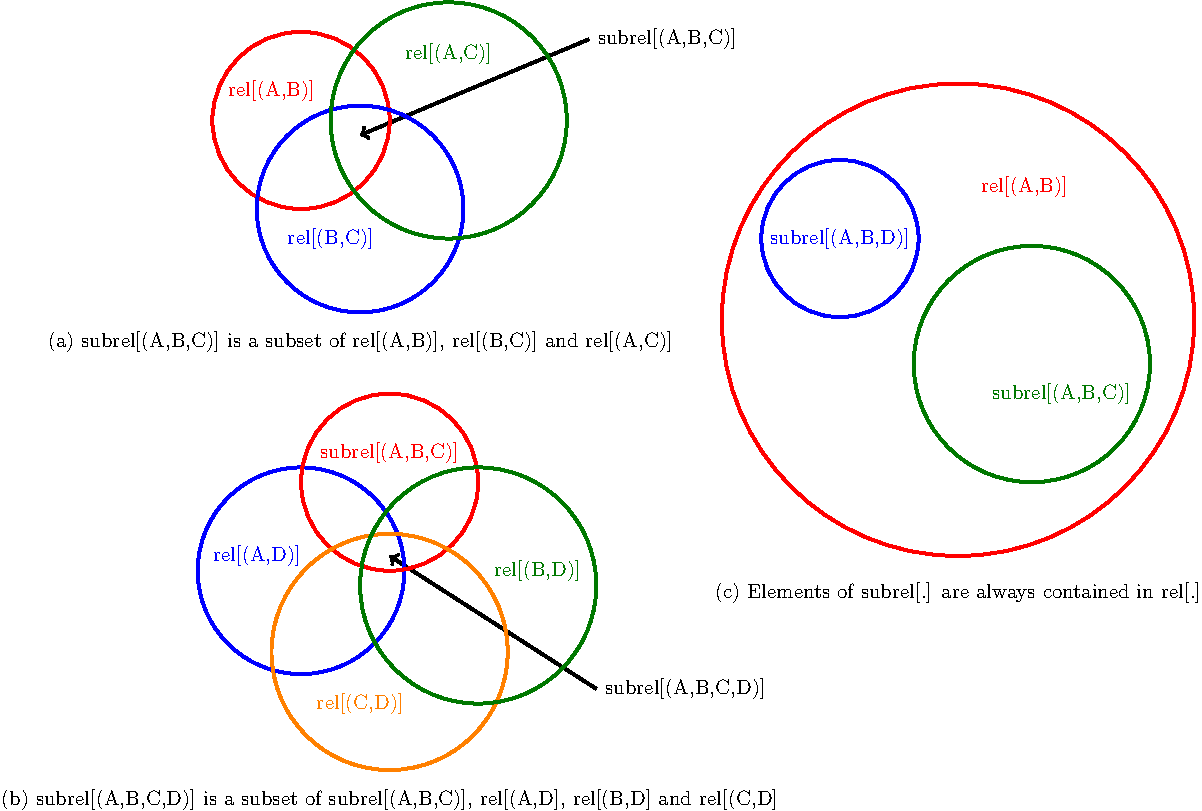
\includegraphics[width=0.5\paperwidth]{../figures/rel_example}
\end{figure}

\begin{thm}
The size of relatives and sub-relatives become smaller with there
are more elements in their identity tuples. \label{theo:size_rel}
\end{thm}
\begin{proof}
We call $\left(\boldsymbol{A},\boldsymbol{B}\right)$ of $\mathrm{rel}\left[\left(\boldsymbol{A},\boldsymbol{B}\right)\right]$,
$\left(\boldsymbol{A},\boldsymbol{B},\boldsymbol{C}\right)$ of $\mathrm{subrel}\left[\left(\boldsymbol{A},\boldsymbol{B},\boldsymbol{C}\right)\right]$,
or such $n$-tuples with $2\leq n\leq U\left(t,3t\right)$ by \textit{identity
tuples}. In Figure \ref{fig:rel_example}(a), we can see that 
\[
\mathrm{subrel}\left[\left(\boldsymbol{A},\boldsymbol{B},\boldsymbol{C}\right)\right]\in\left\{ \mathrm{rel}\left[\left(\boldsymbol{A},\boldsymbol{B}\right)\right]\cap\mathrm{rel}\left[\left(\boldsymbol{A},\boldsymbol{C}\right)\right]\cap\mathrm{rel}\left[\left(\boldsymbol{B},\boldsymbol{C}\right)\right]\right\} ,
\]

which gives us
\[
\begin{array}{c}
\mathrm{subrel}\left[\left(\boldsymbol{A},\boldsymbol{B},\boldsymbol{C}\right)\right]\subseteq\mathrm{rel}\left[\left(\boldsymbol{A},\boldsymbol{B}\right)\right],\\
\mathrm{subrel}\left[\left(\boldsymbol{A},\boldsymbol{B},\boldsymbol{C}\right)\right]\subseteq\mathrm{rel}\left[\left(\boldsymbol{A},\boldsymbol{C}\right)\right],\\
\mathrm{subrel}\left[\left(\boldsymbol{A},\boldsymbol{B},\boldsymbol{C}\right)\right]\subseteq\mathrm{rel}\left[\left(\boldsymbol{B},\boldsymbol{C}\right)\right].
\end{array}
\]
Therefore,
\[
\left|\mathrm{rel}\left[\left(\boldsymbol{A},\boldsymbol{B}\right)\right]\right|\geq\left|\mathrm{subrel}\left[\left(\boldsymbol{A},\boldsymbol{B},\boldsymbol{C}\right)\right]\right|,
\]
which is still true when the size of identity tuples becomes smaller.
\end{proof}
We have tried 2 variants of the above algorithm as following. Firstly,
instead of using \textit{matrix space with unique row space}, we use
the whole matrix space $M\left(n,m\right)$ introduced in Definition
\ref{def:urs_matrix_space}. In case $t=2$, we cover all $2^{3t^{2}}=4096$
matrices instead of only 715 matrices in Section \ref{sec:Main-Approach},
which will help the Algorithm \ref{alg:Increasing-Method} cover the
optimal vector solution.
\begin{defn}[Good Global Coding Vector\label{def:almost_sufficient_global_coding_vector}]
 Let $\boldsymbol{A},\boldsymbol{B},\boldsymbol{C}\in U(t,3t)$ and
$N\leq\left(\begin{array}{c}
2^{3t^{2}}\\
3
\end{array}\right)$, then a set $\mathcal{T}_{n=3t,m=3t}=\left\{ \boldsymbol{T}_{1},\ldots,\boldsymbol{T}_{N}\right\} $
contains distinct \textit{sufficient global coding vectors} $\boldsymbol{T}_{j}$
such that:
\[
\mathrm{rk}\left[\boldsymbol{T}_{j}\right]=\mathrm{rk}\left[\begin{array}{c}
\boldsymbol{A}\\
\boldsymbol{B}\\
\boldsymbol{C}
\end{array}\right]\geq2n,\forall j\in\left\{ 1,\ldots,N\right\} .
\]
In Algorithm \ref{alg:Increasing-Method}, we substitute the input
by $\mathcal{T}_{n=3t,m=3t}$ instead of $\mathcal{H}_{n=3t,m=3t}$.
This will give us an output with upper bound of $\mathcal{A}_{2}\left(3t,2t,3;2t\right)=126$
\cite[Sec. V-B]{Zhang:2019}. We can see that $\left|\mathcal{T}_{n=3t,m=3t}\right|\approx11\cdot10^{9}\gg\left|\mathcal{H}_{n=3t,m=3t}\right|\approx60\cdot10^{6}$.
\end{defn}
Secondly, we tried another approach called ``Randomly Increasing
Method''. We got about 72 codewords instead of 89 codewords as Algorithm
\ref{alg:Increasing-Method}, due to a limited number of tries. Briefly,
this approach started with a pair of the following 2 potential matrices
\[
\left[\begin{array}{cccccc}
0 & 0 & 0 & 0 & 0 & 0\\
0 & 0 & 0 & 0 & 0 & 0
\end{array}\right],\left[\begin{array}{cccccc}
1 & 0 & 0 & 0 & 0 & 0\\
0 & 1 & 0 & 0 & 0 & 0
\end{array}\right].
\]
Then we tried adding a new random matrix from $U\left(t=2,3t=6\right)$
into a list containing this pair. The random matrix is extended to
the list, if the matrix and any 2 existing matrices in the list satisfy
(\ref{eq:rk_rqm_e1l1h3s4}). The list will be extended until all matrices
in $U\left(t=2,3t=6\right)$ are checked.

\section{Decremental Algorithm (DM) \label{sec:Alternative-Approaches}}

In Algorithm \ref{alg:Decreasing-Method}, we introduce a decremental
algorithm by removing bad matrices from a set of 715 matrices, until
any 3 of the matrices left in the set satisfy (\ref{eq:rk_rqm_e1l1h3s4}).
A matrix with the less number of occurence in $\mathcal{T}_{n=3t,m=3t}$
or $\mathcal{H}_{n=3t,m=3t}$ is evaluated as a bad matrix, and it
is removed for each step. If many bad matrices exist, we only remove
the first one, which makes this algorithm a random one and require
multiple tries. In case $t=2$, we tried once with $\left|U\left(t,3t\right)\right|=715$
matrices as the algorithm's input, and unfortunately got about 69
codewords instead of 89 codewords as Algorithm \ref{alg:Increasing-Method}. 

\begin{algorithm}[H]
\caption{Decreasing Method \label{alg:Decreasing-Method}}

\hspace*{\algorithmicindent} \textbf{Input}: $U(t,3t)$. \\
\hspace*{\algorithmicindent} \textbf{Output}: A subset of $U(t,3t)$ with any 3 matrices satisfy Equation \ref{eq:p_in_LLL}. 
\begin{algorithmic}[1]
	\STATE {$\left[\textbf{L}_{0},\ldots,\boldsymbol{L}_{\left|U(t,3t)\right|-1}\right]\leftarrow U(t,3t)$ // Assign all matrices into a list.}
	\STATE {$\boldsymbol{j}\leftarrow\left[\boldsymbol{L}_{0},\ldots,\boldsymbol{L}_{\left|U(t,3t)\right|-1}\right]$}
	\REPEAT
	\STATE {$\boldsymbol{g}\leftarrow\left[0,\ldots,0\right]$ with $\left|\boldsymbol{g}\right|=\left|\boldsymbol{j}\right|$ // Number of occurences for bad matrices}
	\FORALL{$\left[c_{0},c_{1},c_{2}\right]\in\left(\begin{array}{c} \left|\boldsymbol{j}\right|\\ 3 \end{array}\right)$}
		\IF{$rk\left[\begin{array}{c} \boldsymbol{j}_{c_{0}}\\ \boldsymbol{j}_{c_{1}}\\ \boldsymbol{j}_{c_{2}} \end{array}\right]\leq2t$}	
			\STATE {$\textbf{g}_{c_{0}}\leftarrow \textbf{g}_{c_{0}}+1$}
			\STATE {$\textbf{g}_{c_{1}}\leftarrow \textbf{g}_{c_{1}}+1$}
			\STATE {$\textbf{g}_{c_{2}}\leftarrow \textbf{g}_{c_{2}}+1$}
		\ENDIF
	\ENDFOR
	\STATE {remove $\boldsymbol{j}_{max\left[\boldsymbol{g}\right]\neq0}$ from $\boldsymbol{j}$}
	\UNTIL{$max\left[\boldsymbol{g}\right]=0$}
\end{algorithmic}
\end{algorithm}
Finally, construction 1 mentioned in Section \ref{sec:Main-Approach}
to achieve a vector solution for the $\left(1,1\right)-\mathcal{N}_{3,r,4}$
network with $t=3$, which has not been yet found in any other papers.
When $t=3$, a $3-\left(9,3,3\right)_{4}^{c}$ code is required for
a vector solution of the network by Theorem \ref{theo:scalar_sol_exist}.
Its orthogonal complement is a $3-\left(9,6,2\right)_{q}^{m}$ code,
and the bound for this code is denoted by $\mathcal{A}_{2}\left(9,6,3;2\right)$
following to Corollary \ref{cor:dual_subspaces}. In \cite{Etzion:2018},
they only covered $\mathcal{A}_{2}\left(6,k,t;2\right),\mathcal{A}_{2}\left(7,k,t;2\right)$,
and $\mathcal{A}_{2}\left(8,k,t;2\right)$, this is thus a newly found
bound for a vector solution of the $\left(1,1\right)-\mathcal{N}_{3,r,4}$
network. We listed 166 three-dimensional subspaces of $\ensuremath{\mathbb{F}}_{2}^{9}$
in Appendix \ref{sec:166-Three-Dimensional-Subspaces}. Therefore,
we conclude $166\leq\mathcal{A}_{2}\left(9,6,3;2\right)$. By Theorem
\ref{theo:zhang-theorem10}, we achieve its upper bound $\mathcal{A}_{2}\left(9,6,3;2\right)\leq1129$.
The upper bound can be improved by Theorem \ref{theo:zhang-theorem11}
with $\mathcal{A}_{2}\left(9,6,3;2\right)\leq\left\lfloor \frac{85}{21}\mathcal{A}_{2}\left(8,5,2;2\right)\right\rfloor \leq537$,
where $33\leq\mathcal{A}_{2}\left(8,5,2;2\right)\leq128$ in \cite[Table 3]{Etzion:2018}.
Hence, we have $166\leq\mathcal{A}_{2}\left(9,6,3;2\right)\leq537$.
\begin{thm}[{\cite[Theorem 10]{Zhang:2019}\label{theo:zhang-theorem10}}]
 If $n,k,\mathrm{t}$ and $\lambda$ are positive integers such that
$1\leq\mathrm{t}<k<n$ and $1\leq\lambda\leq\left[\begin{array}{c}
n-\mathrm{t}\\
k-\mathrm{t}
\end{array}\right]_{q}$, then,
\[
\mathcal{A}_{q}\left(n,k,\mathrm{t};\lambda\right)\leq\left\lfloor \lambda\frac{\left[\begin{array}{c}
n\\
\mathrm{t}
\end{array}\right]_{q}}{\left[\begin{array}{c}
k\\
\mathrm{t}
\end{array}\right]_{q}}\right\rfloor 
\]
\end{thm}
%
\begin{thm}[{\cite[Theorem 11]{Zhang:2019}\label{theo:zhang-theorem11}}]
 If $n,k,\mathrm{t}$ and $\lambda$ are positive integers such that
$1\leq\mathrm{t}<k<n$ and $1\leq\lambda\leq\left[\begin{array}{c}
n-\mathrm{t}\\
k-\mathrm{t}
\end{array}\right]_{q}$, then,
\[
\mathcal{A}_{q}\left(n,k,\mathrm{t};\lambda\right)\leq\left\lfloor \frac{q^{n}-1}{q^{k}-1}\mathcal{A}_{q}\left(n-1,k-1,\mathrm{t}-1;\lambda\right)\right\rfloor 
\]

\newpage{}
\end{thm}
\begin{sidewaystable}[H]
\begin{centering}
\begin{tabular}{|c|c|c|c|c|c|}
\hline 
t & Scalar Solution ({*}) & Vector Solution ({*}) & Etzion and Kurz & Construction 1 (IM) & Construction 2 (IM)\tabularnewline
\hline 
\hline 
2 & $r_{\mathrm{max,scalar}}=42$ & $r_{\mathrm{max,vector}}\geq7$ & $r_{\mathrm{max,vector}}=121$ & $r_{\mathrm{max,vector}}=89$ & N/A\tabularnewline
\hline 
3 & $r_{\mathrm{max,scalar}}=146$ & $r_{\mathrm{max,vector}}\geq62$  & N/A & N/A & $r_{\mathrm{max,vector}}=166$\tabularnewline
\hline 
4 & $r_{\mathrm{max,scalar}}=546$ & $r_{\mathrm{max,vector}}\geq1317$ & N/A & N/A & N/A\tabularnewline
\hline 
5 & $r_{\mathrm{max,scalar}}=2114$ & $r_{\mathrm{max,vector}}\geq58472$ & N/A & N/A & N/A\tabularnewline
\hline 
6 & $r_{\mathrm{max,scalar}}=8322$ & $r_{\mathrm{max,vector}}>10^{6}$ & N/A & N/A & N/A\tabularnewline
\hline 
\end{tabular}
\par\end{centering}
\centering{}\caption{Vector solutions outperform the optimal scalar solution for the $\left(\epsilon=1,\ell=1\right)-\mathcal{N}_{h=3,r,s=4}$
network over $t=2,\ldots,6$. For $t=2$, the vector solution found
in \cite{Etzion:2018} gives the largest number of the intermediate
nodes with $r_{\mathrm{max,vector}}=121$. For $t=3$, our vector
solution gives a better result than both the optimal scalar solution
and the combinatorial vector solution with $r_{\mathrm{max,vector}}=166$.
For $t=3,\ldots,6$, all of our combinatorial vector solutions outperform
the optimal scalar one. ({*}): combinatorial results based on Table
\ref{tab:r_over_t}.\label{tab:r_over_t-1}}
\end{sidewaystable}


\part{Conclusion}

In this thesis, we have shown combinatorial proofs for an existence
of new gaps for 3 generalized combination networks. The $\left(\epsilon=1,\ell=1\right)-\mathcal{N}_{h=3,r,s=4}$
network with $t=2$ has been studied in \cite{Wachter-Zeh:2018,Etzion:2016,Zhang:2019,Etzion:2018}
but no general gap was found. We also got computational results for
this network with 89 two-dimensional subspaces of $\ensuremath{\mathbb{F}}_{2}^{6}$,
which is better the constructed set of 51 two-dimensional subspaces
of $\ensuremath{\mathbb{F}}_{2}^{6}$ found in \cite{Wachter-Zeh:2018}.

In Chapter 5, by applying the Local lemma, we stated that there is
an $r_{\mathrm{max,vector}}\in\Omega\left(q^{t^{2}/2+\mathcal{O}\left(t\right)}\right)$
such that for any $r\leq r_{\mathrm{max,vector}}$ there exists a
vector solution for the $\left(\epsilon=1,l=1\right)-\mathcal{N}_{h=3,r,s=4}$
network. The optimal scalar solution for such network exists, when
$r\leq\mathcal{O}\left(q_{\mathrm{s}}^{2}\right)$. Therefore, a lower
bound on the gap $g_{\mathrm{lower\,bound}}=q^{t^{2}/4+\mathcal{O}(t)}$
exists for the $\left(1,1\right)-\mathcal{N}_{3,r,4}$ network. Similarly
we derived the gaps for the $\left(\epsilon=1,\ell=1\right)-\mathcal{N}_{h,r,s}$
network, the $\left(\epsilon>1,\ell=1\right)-\mathcal{N}_{h,r,s}$
network and the $\left(\epsilon=1,\ell>1\right)-\mathcal{N}_{h=2\ell,r,s=2\ell+1}$
network, respectively with the following gap 
\[
\begin{array}{c}
g_{\mathrm{lower\,bound}}=q^{\frac{\alpha-h+1}{\left(\alpha-1\right)\left(\alpha-h+2\right)\left(h-2\right)}t^{2}+\mathcal{O}(t)},\\
g_{\mathrm{lower\,bound}}=q^{\frac{\epsilon\left(\alpha-h+\epsilon\right)}{\left(\alpha-1\right)\left(\alpha-h+\epsilon+1\right)\left(h-\epsilon-1\right)}t^{2}+\mathcal{O}(t)},\\
g_{\mathrm{lower\,bound}}=q^{t^{2}/2\ell+\mathcal{O}(t)}.
\end{array}
\]
A comparison with known results can be found in Table \ref{tab:New-gap-found}
and Table \ref{tab:r_over_t}.

In Chapter 6, we introduced 4 different approaches in computing vector
solutions that outperform the optimal scalar solution for the $\left(\epsilon=1,\ell=1\right)-\mathcal{N}_{h=3,r,s=4}$
network with $t=2$. All approaches gave us such vector solutions,
and the Algorithm \ref{alg:Increasing-Method} called ``Increasing
Method'' generated the best result among 4 approaches. The best result
is about 2 times 42 results of the optimal scalar solution, i.e. we
found $r_{vector}=89$. When we mention the results of the optimal
scalar solution, it means that such a solution exists if and only
if $r_{scalar}\leq42$. However, our computational result of $r_{vector}$
is still less than the upper bound of $\mathcal{A}_{2}\left(6,4,3;2\right)$
in \cite{Etzion:2018}. Hence, we can only conclude $89\leq\mathcal{A}_{2}\left(6,4,3;2\right)\leq126$
for the $\left(\epsilon=1,\ell=1\right)-\mathcal{N}_{h=3,r,s=4}$
network with $t=2$. This motivates an open research to find a computational
method for generating a vector solution of 126 two-dimensional subspaces
of $\ensuremath{\mathbb{F}}_{2}^{6}$. At the time writing this thesis,
the best computational result is $r_{vector}=121$ stated in \cite{Etzion:2018}.
In Appendix \ref{sec:89-Two-Dimensional-Subspaces}, we listed one
of 2 different sets of our 89 two-dimensional subspaces of $\ensuremath{\mathbb{F}}_{2}^{6}$,
which are slightly different in 2 subspaces. We also find an interesting
result that there are $\left|U(2,6)\right|=715$ matrices whose different
row spaces among $\left|M(2,6)\right|=4096$ matrices over $\ensuremath{\mathbb{F}}_{2}^{6}$.
Furthermore, we used the Algorithm \ref{alg:Increasing-Method} and
got $r_{vector}=166$ for $t=3$ by Construction 1, which is better
than the optimal scalar solution existing if and only $r_{scalar}\leq146$.
This computational result was not found in any previous studies in
our scope of knowledge. For the $\left(\epsilon=1,\ell=1\right)-\mathcal{N}_{h=3,r,s=4}$
network with $t=3$, we therefore state a new bound $166\leq\mathcal{A}_{2}\left(9,6,3;2\right)\leq537$.
In Appendix \ref{sec:166-Three-Dimensional-Subspaces}, we wrote down
one of 18 found variants of 166 three-dimensional subspaces of $\ensuremath{\mathbb{F}}_{2}^{9}$.
From $\left|M(3,6)\right|=262144$ matrices, we found $\left|U(3,6)\right|=2110$
matrices whose different row spaces. All of computational results
in this study was listed in Table \ref{tab:r_over_t}. 

Another open research is to study a gap for the general network $\left(\epsilon,\ell\right)-\mathcal{N}_{h,r,s}$
with $\left(\epsilon>1,\ell>1\right)$ or $\left(\epsilon=1,\ell>1\right)$
for any $\alpha\geq1$. The most challenging problem for such research
is to define the optimal scalar solution for such network.

\part{Appendices}

\section{Proofs of Theorem \ref{theo:e2l1_r_max_vector}, Theorem \ref{theo:e2l1_r_max_scalar}
and Corollary \ref{cor:e2l1_gap} \label{app:proofs_e2l1}}
\begin{proof}[Proof of Theorem \vref{theo:e2l1_r_max_vector}]
 As in Section \vref{sec:e1l1_nw}, there exists a vector solution
for the $\left(\epsilon>1,\ell=1\right)-\mathcal{N}_{h,r,s}$ network
if
\[
\mathrm{rk}\left[\begin{array}{c}
\boldsymbol{A}^{\left(r_{1}\right)}\\
\vdots\\
\boldsymbol{A}^{\left(r_{\alpha}\right)}
\end{array}\right]\geq\left(h-\epsilon\right)t.
\]
Similar to Lemma \ref{lem:p_e1l1}, we have $p\in\Theta\left(q^{\left(\epsilon h-\epsilon\alpha-\epsilon^{2}\right)t^{2}+\mathcal{O}(t)}\right)$.
And there is no difference for $d$, we then have $r_{\mathrm{max,vector}}\in\Omega\left(q^{\frac{\epsilon\left(h-\alpha-\epsilon\right)}{1-\alpha}t^{2}+\mathcal{O}(t)}\right)$
following to the Local lemma \ref{thm:LLL}.
\end{proof}
%
\begin{proof}[Proof of Theorem \vref{theo:e2l1_r_max_scalar}]
 As in the proof of Theorem \ref{theo:r_scalar_e1l1}, there exists
a scalar solution for the $\left(\epsilon>1,\ell=1\right)-\mathcal{N}_{h,r,s}$
network if

\begin{eqnarray*}
 & r & \leq\left(\alpha-1\right)\stackrel[i=0]{h-\epsilon-2}{\prod}\frac{q_{\mathrm{s}}^{\alpha}-q_{\mathrm{s}}^{i}}{q_{\mathrm{s}}^{h-\epsilon-1}-q_{\mathrm{s}}^{i}}\approx\left(\alpha-1\right)\left(q_{\mathrm{s}}^{\left(\alpha-h+\epsilon+1\right)\left(h-\epsilon-1\right)}\right)\\
\Rightarrow & r_{\mathrm{max,scalar}} & \in\mathcal{O}\left(q_{\mathrm{s}}^{\left(\alpha-h+\epsilon+1\right)\left(h-\epsilon-1\right)}\right).
\end{eqnarray*}

Hence, there exists such $r_{\mathrm{max,scalar}}$ such that for
any $r\leq r_{\mathrm{max,scalar}}$there exists a scalar solution
for the network.
\end{proof}
%
\begin{proof}[Proof of Corollary \vref{cor:e2l1_gap}]
 The gap follows by applying Section \ref{subsec:Comparison-between-scalar-and-vector-sol}
with Theorem \vref{theo:e2l1_r_max_vector} and Theorem \vref{theo:e2l1_r_max_scalar}.
\end{proof}

\section{89 Two-Dimensional Subspaces of $\ensuremath{\mathbb{F}}_{2}^{6}$
for the $\left(\epsilon=1,\ell=1\right)-\mathcal{N}_{h=3,r,s=4}$
Network \label{sec:89-Two-Dimensional-Subspaces}}

By applying Algorithm \vref{alg:Increasing-Method} with details mentioned
in Section (\ref{sec:Main-Approach}), we computed the following 89
subspaces of $\ensuremath{\mathbb{F}}_{2}^{6}$ for our vector solution
for the $\left(\epsilon=1,\ell=1\right)-\mathcal{N}_{h=3,r,s=4}$
network, which are equivalently to 89 intermediate nodes in the middle
layer of the network.

\begin{lstlisting}
[1 0 0 0 0 0] [1 0 0 0 0 0] [0 0 1 0 0 0] [0 0 0 1 0 0] 
[0 1 0 0 0 0] [0 0 1 0 0 0] [0 0 0 0 0 1] [0 0 0 0 1 0] 

[1 0 0 0 1 0] [1 0 0 0 0 0] [1 0 0 0 0 0] [0 1 0 0 1 0] 
[0 0 0 0 0 1] [0 0 1 0 1 0] [0 0 0 1 0 1] [0 0 0 1 0 0] 

[0 1 0 0 0 1] [0 0 1 0 0 1] [0 0 0 1 0 1] [1 1 1 0 0 0] 
[0 0 1 0 0 0] [0 0 0 1 0 0] [0 0 0 0 1 0] [0 0 0 0 1 0] 

[1 0 1 0 0 0] [1 0 1 0 0 0] [1 0 1 0 0 0] [1 0 0 1 0 0] 
[1 0 0 1 0 0] [0 1 0 1 0 0] [0 0 0 1 1 0] [1 0 0 0 0 1] 

[1 0 0 0 1 1] [1 0 0 0 1 0] [1 0 0 0 0 1] [0 1 1 1 0 0] 
[0 0 0 1 0 0] [1 0 0 0 0 1] [0 1 0 1 0 0] [0 0 0 0 1 0] 

[0 1 1 0 0 0] [0 1 1 0 0 0] [0 1 0 0 0 1] [0 1 0 0 0 0] 
[0 1 0 0 1 0] [0 0 0 1 0 1] [0 0 1 1 0 0] [0 0 1 1 1 0] 

[0 0 1 1 1 0] [0 0 1 1 0 0] [1 1 1 0 0 0] [1 1 1 0 0 0] 
[0 0 0 0 0 1] [0 0 0 0 1 1] [1 0 0 0 1 0] [0 1 0 1 0 0] 

[1 1 0 1 0 0] [1 1 0 0 1 0] [1 1 0 0 1 0] [1 1 0 0 0 1] 
[0 1 0 0 1 0] [0 1 0 1 0 0] [0 1 0 0 0 1] [1 0 0 1 0 0] 

[1 1 0 0 0 0] [1 1 0 0 0 0] [1 0 1 1 1 0] [1 0 1 1 0 0] 
[1 0 1 0 0 1] [0 0 0 1 1 1] [0 0 0 0 0 1] [0 1 0 0 0 1] 

[1 0 1 1 0 0] [1 0 1 0 1 1] [1 0 1 0 1 1] [1 0 0 1 1 0] 
[0 0 1 0 0 1] [0 1 0 0 0 0] [0 0 0 1 0 0] [0 0 0 0 1 1] 

[1 0 0 0 0 1] [0 1 1 0 0 1] [0 1 0 1 1 1] [0 0 1 1 0 1] 
[0 1 0 1 1 0] [0 0 1 0 1 0] [0 0 1 0 0 0] [0 0 1 0 1 0] 

[0 0 1 1 0 0] [1 1 1 1 1 0] [1 1 1 1 0 0] [1 1 1 0 1 0] 
[0 0 1 0 1 1] [0 0 0 0 0 1] [0 1 0 0 0 1] [0 0 1 0 0 1] 

[1 1 1 0 0 1] [1 1 0 1 1 0] [1 1 0 1 0 1] [1 1 0 1 0 0] 
[0 0 0 1 1 0] [1 0 1 0 0 0] [0 1 1 0 0 0] [1 0 0 0 1 1] 

[1 1 0 1 0 0] [1 1 0 0 1 1] [1 1 0 0 1 1] [1 1 0 0 1 0] 
[0 0 1 1 0 1] [0 1 1 0 0 0] [0 0 1 1 0 0] [0 1 1 1 0 0] 

[1 1 0 0 0 1] [1 1 0 0 0 1] [1 0 1 1 0 0] [1 0 1 1 0 0] 
[1 0 1 0 1 0] [0 1 1 0 1 0] [0 1 0 1 0 1] [0 0 0 1 1 1] 

[1 0 1 0 1 0] [1 0 1 0 0 1] [1 0 1 0 0 1] [1 0 0 1 1 0] 
[0 1 0 1 1 0] [0 1 1 1 0 0] [0 1 0 1 0 1] [0 1 0 1 0 1] 

[1 0 0 1 0 1] [1 0 0 1 0 1] [1 0 0 0 0 1] [0 1 1 1 0 1] 
[0 1 1 0 1 0] [0 0 1 0 1 1] [0 1 1 1 1 0] [0 0 0 1 1 0] 

[0 1 1 0 1 1] [0 1 1 0 0 1] [0 1 0 1 0 1] [0 1 0 0 1 1] 
[0 1 0 1 0 0] [0 1 0 1 1 0] [0 0 1 0 1 1] [0 0 1 1 1 0] 

[1 1 1 1 1 0] [1 1 1 1 1 0] [1 1 1 1 0 0] [1 1 1 0 0 1] 
[0 0 0 1 0 1] [0 0 0 0 1 1] [0 1 0 0 1 1] [0 0 1 1 1 0] 

[1 1 0 1 1 0] [1 1 0 1 1 0] [1 1 0 1 0 1] [1 1 0 1 0 0] 
[1 0 1 0 0 1] [0 0 1 1 0 1] [0 0 1 0 1 1] [0 1 1 0 1 1] 

[1 1 0 0 1 1] [1 1 0 0 0 1] [1 0 1 1 0 1] [1 0 1 0 1 0] 
[0 0 1 1 1 0] [1 0 1 1 1 0] [0 1 1 0 1 0] [0 1 0 1 1 1] 

[1 0 0 1 1 1] [1 0 0 1 1 1] [1 1 1 0 1 0] [1 1 1 0 1 0] 
[0 1 1 1 0 0] [0 1 1 0 1 0] [1 0 1 1 0 1] [1 0 0 1 1 1] 

[1 1 0 1 1 0] 
[1 0 1 1 0 1]
\end{lstlisting}


\section{166 Three-Dimensional Subspaces of $\ensuremath{\mathbb{F}}_{2}^{9}$
for the $\left(\epsilon=1,\ell=1\right)-\mathcal{N}_{h=3,r,s=4}$
Network \label{sec:166-Three-Dimensional-Subspaces}}

By applying Algorithm \vref{alg:Increasing-Method} with details mentioned
in Section (\ref{sec:Main-Approach}), we computed the following 166
subspaces of $\ensuremath{\mathbb{F}}_{2}^{9}$ for our vector solution
for the $\left(\epsilon=1,\ell=1\right)-\mathcal{N}_{h=3,r,s=4}$
network, which are equivalently to 166 intermediate nodes in the middle
layer of the network. A vector solution over $\ensuremath{\mathbb{F}}_{2}^{9}$
for the $\left(\epsilon=1,\ell=1\right)-\mathcal{N}_{h=3,r,s=4}$
network has not yet been studied in any other studies.

\begin{lstlisting}
[1 0 0 0 0 1 0 0 0] [1 0 0 0 0 0 1 0 0] 
[0 1 0 0 0 0 0 1 0] [0 1 0 0 0 0 0 0 1] 
[0 0 1 0 0 0 0 0 0] [0 0 1 0 0 0 0 0 0] 

[1 0 0 1 0 1 0 1 0] [1 0 0 1 1 0 1 0 1] 
[0 1 0 1 0 0 1 0 0] [0 1 0 1 0 1 0 0 0] 
[0 0 1 0 0 0 0 1 1] [0 0 1 0 0 0 0 1 0] 

[1 0 0 1 0 0 1 0 0] [1 0 0 0 0 1 1 1 0] 
[0 1 0 0 1 1 0 1 0] [0 1 0 0 0 0 0 1 1] 
[0 0 1 0 0 0 0 0 1] [0 0 1 0 0 0 0 0 0] 

[1 0 0 1 0 1 0 1 0] [1 0 0 0 0 1 1 0 1] 
[0 1 0 0 1 1 1 0 0] [0 1 0 0 0 0 1 1 0] 
[0 0 1 0 1 0 0 0 1] [0 0 1 0 0 0 0 0 0] 

[1 0 0 1 1 0 0 0 0] [1 0 0 1 0 1 0 1 0] 
[0 1 0 0 0 0 0 1 0] [0 1 0 0 1 0 1 1 0] 
[0 0 1 0 0 0 0 0 0] [0 0 1 0 0 0 1 0 1] 

[1 0 0 1 0 0 0 1 0] [1 0 0 1 0 0 0 0 1] 
[0 1 0 0 0 1 0 0 0] [0 1 0 0 0 0 1 0 0] 
[0 0 1 0 0 0 0 0 0] [0 0 1 0 0 0 0 0 0] 

[1 0 0 1 1 0 1 0 0] [1 0 0 1 0 0 0 0 0] 
[0 1 0 1 0 1 0 1 0] [0 1 0 0 1 0 0 0 1] 
[0 0 1 0 0 0 0 1 1] [0 0 1 0 0 0 0 0 0] 

[1 0 0 1 0 0 0 0 0] [1 0 0 1 0 0 0 0 0] 
[0 1 0 0 1 0 0 0 0] [0 1 0 0 0 1 0 0 0] 
[0 0 1 0 0 1 0 0 0] [0 0 1 0 0 0 1 0 0] 

[1 0 0 1 0 0 0 0 0] [1 0 0 0 1 0 0 1 0] 
[0 1 0 0 0 0 1 0 0] [0 1 0 0 0 0 0 0 1] 
[0 0 1 0 0 0 0 1 0] [0 0 1 0 0 0 0 0 0] 

[1 0 0 1 1 0 0 1 0] [1 0 0 0 1 0 0 0 0] 
[0 1 0 1 0 0 1 0 1] [0 1 0 0 0 1 0 0 0] 
[0 0 1 0 1 1 0 0 1] [0 0 1 0 0 0 1 0 0] 

[1 0 0 0 1 0 0 0 0] [1 0 0 1 1 0 1 0 0] 
[0 1 0 0 0 0 1 1 0] [0 1 0 1 0 0 0 1 0] 
[0 0 1 0 0 0 0 0 0] [0 0 1 1 0 0 0 0 1] 

[1 0 0 0 0 1 0 1 0] [1 0 0 1 1 0 0 0 1] 
[0 1 0 0 0 0 1 0 0] [0 1 0 0 1 1 0 0 0] 
[0 0 1 0 0 0 0 0 0] [0 0 1 0 0 0 1 1 1] 

[1 0 0 1 1 0 1 0 0] [1 0 0 1 0 0 0 1 1] 
[0 1 0 0 1 1 0 0 0] [0 1 0 0 1 0 1 0 0] 
[0 0 1 0 1 0 0 0 1] [0 0 1 0 0 1 0 0 0] 

[1 0 0 1 1 0 1 0 0] [1 0 0 0 0 0 1 0 0] 
[0 1 0 0 0 1 1 1 1] [0 1 0 0 0 0 0 1 0] 
[0 0 1 0 0 0 0 0 0] [0 0 1 0 0 0 0 0 1] 

[1 0 0 0 0 1 0 1 0] [1 0 0 1 1 0 1 1 0] 
[0 1 0 0 0 1 0 0 1] [0 1 0 1 0 1 0 0 0] 
[0 0 1 0 0 0 1 0 0] [0 0 1 0 1 0 0 0 1] 

[1 0 0 1 0 0 0 1 0] [1 0 0 1 1 0 0 1 1] 
[0 1 0 1 0 0 0 0 1] [0 1 0 1 0 0 1 0 0] 
[0 0 1 0 1 1 0 0 0] [0 0 1 0 0 1 0 0 0] 

[1 0 0 1 0 1 0 0 1] [1 0 0 1 1 0 1 1 0] 
[0 1 0 1 0 0 0 1 0] [0 1 0 0 1 1 0 0 0] 
[0 0 1 0 1 0 1 0 1] [0 0 1 0 0 0 1 0 1] 

[1 0 0 1 0 1 0 0 1] [1 0 0 1 0 1 0 0 1] 
[0 1 0 0 1 1 1 0 0] [0 1 0 0 1 1 0 1 0] 
[0 0 1 0 0 0 1 1 0] [0 0 1 0 1 0 1 0 0] 

[1 0 0 1 0 1 0 1 0] [1 0 0 1 1 0 1 0 1] 
[0 1 0 0 1 0 0 0 1] [0 1 0 0 0 0 0 0 0] 
[0 0 1 0 0 1 1 0 0] [0 0 1 0 0 0 0 0 0] 

[1 0 0 1 0 1 0 0 1] [1 0 0 1 1 0 0 1 0] 
[0 1 0 0 1 0 1 0 1] [0 1 0 1 0 1 1 0 0] 
[0 0 1 0 0 1 0 1 0] [0 0 1 0 1 1 0 0 1] 

[1 0 0 1 0 1 0 0 0] [1 0 0 1 1 0 0 1 0] 
[0 1 0 0 1 0 0 0 0] [0 1 0 0 1 1 0 0 0] 
[0 0 1 0 0 0 0 1 0] [0 0 1 0 1 0 1 0 0] 

[1 0 0 1 1 0 0 1 0] [1 0 0 1 0 0 1 0 0] 
[0 1 0 0 1 0 1 0 0] [0 1 0 0 1 1 0 0 0] 
[0 0 1 0 1 0 0 0 1] [0 0 1 0 0 0 0 0 0] 

[1 0 0 1 0 0 0 1 0] [1 0 0 1 1 0 1 0 1] 
[0 1 0 0 1 0 0 0 0] [0 1 0 0 1 1 0 0 0] 
[0 0 1 0 0 0 0 0 1] [0 0 1 0 1 0 0 1 0] 

[1 0 0 1 1 0 0 0 1] [1 0 0 1 1 0 0 0 1] 
[0 1 0 1 0 1 1 1 0] [0 1 0 1 0 1 0 0 0] 
[0 0 1 0 0 0 0 0 0] [0 0 1 1 0 0 1 0 0] 

[1 0 0 1 1 0 0 0 1] [1 0 0 1 0 0 0 1 1] 
[0 1 0 1 0 0 0 1 0] [0 1 0 0 1 1 0 1 0] 
[0 0 1 0 1 1 0 0 0] [0 0 1 0 1 0 1 0 0] 

[1 0 0 1 1 0 0 0 1] [1 0 0 1 1 0 0 0 1] 
[0 1 0 0 1 1 0 1 0] [0 1 0 0 1 0 1 1 0] 
[0 0 1 0 0 0 1 0 0] [0 0 1 0 0 1 0 0 0] 

[1 0 0 0 1 1 0 0 0] [1 0 0 1 0 1 0 0 0] 
[0 1 0 0 1 0 0 0 1] [0 1 0 1 0 0 0 1 1] 
[0 0 1 0 0 0 0 0 0] [0 0 1 0 1 0 1 1 0] 

[1 0 0 0 1 0 1 0 0] [1 0 0 1 1 0 1 0 0] 
[0 1 0 0 0 1 0 0 0] [0 1 0 1 0 1 0 0 0] 
[0 0 1 0 0 0 0 0 1] [0 0 1 0 0 0 1 1 1] 

[1 0 0 1 0 0 0 0 0] [1 0 0 1 1 0 0 0 1] 
[0 1 0 0 1 1 0 1 0] [0 1 0 1 0 1 0 1 0] 
[0 0 1 0 0 1 1 0 0] [0 0 1 0 1 1 1 0 0] 

[1 0 0 1 1 0 0 0 1] [1 0 0 1 0 0 0 0 0] 
[0 1 0 1 0 1 0 1 0] [0 1 0 0 1 0 1 0 0] 
[0 0 1 0 1 0 1 1 0] [0 0 1 0 1 0 0 1 1] 

[1 0 0 1 1 0 0 0 0] [1 0 0 1 1 0 0 0 0] 
[0 1 0 1 0 1 1 0 0] [0 1 0 1 0 1 0 1 0] 
[0 0 1 0 0 1 0 0 1] [0 0 1 0 0 1 1 0 0] 

[1 0 0 1 1 0 0 0 0] [1 0 0 1 0 0 0 0 0] 
[0 1 0 1 0 1 0 0 1] [0 1 0 0 1 1 1 0 1] 
[0 0 1 1 0 0 0 1 0] [0 0 1 0 1 0 0 1 0] 

[1 0 0 0 1 0 0 0 0] [1 0 0 1 0 0 0 0 0] 
[0 1 0 0 0 0 1 0 0] [0 1 0 0 0 1 1 0 1] 
[0 0 1 0 0 0 0 1 1] [0 0 1 0 0 0 1 1 0] 

[1 0 0 1 1 0 0 0 0] [1 0 0 1 0 0 0 0 0] 
[0 1 0 1 0 0 1 0 1] [0 1 0 0 1 1 0 0 1] 
[0 0 1 1 0 0 0 1 0] [0 0 1 0 0 1 1 1 0] 

[1 0 0 0 0 1 1 0 0] [1 0 0 1 0 1 0 0 0] 
[0 1 0 0 0 1 0 1 0] [0 1 0 1 0 0 1 0 1] 
[0 0 1 0 0 0 0 0 0] [0 0 1 0 1 0 0 1 1] 

[1 0 0 1 0 1 0 0 1] [1 0 0 1 0 1 0 0 1] 
[0 1 0 1 0 0 1 1 0] [0 1 0 1 0 0 1 1 0] 
[0 0 1 0 1 1 1 0 0] [0 0 1 0 1 1 0 1 0] 

[1 0 0 0 1 1 1 1 0] [1 0 0 1 1 0 0 1 0] 
[0 1 0 0 0 1 0 0 1] [0 1 0 1 0 1 0 0 1] 
[0 0 1 0 0 0 0 0 0] [0 0 1 0 0 1 1 0 0] 

[1 0 0 1 1 0 0 1 1] [1 0 0 0 1 0 1 0 0] 
[0 1 0 1 0 1 1 0 1] [0 1 0 0 1 0 0 1 1] 
[0 0 1 0 0 0 0 0 0] [0 0 1 0 0 1 0 0 0] 

[1 0 0 0 1 1 1 0 0] [1 0 0 0 0 0 1 1 0] 
[0 1 0 0 0 0 1 1 0] [0 1 0 0 0 0 1 0 1] 
[0 0 1 0 0 0 0 0 1] [0 0 1 0 0 0 0 0 0] 

[1 0 0 0 1 1 0 1 0] [1 0 0 1 0 0 1 1 0] 
[0 1 0 0 0 1 1 0 0] [0 1 0 1 0 0 0 0 1] 
[0 0 1 0 0 0 0 0 1] [0 0 1 0 1 1 0 1 0] 

[1 0 0 1 0 1 1 0 1] [1 0 0 0 1 1 0 0 1] 
[0 1 0 0 1 0 1 1 0] [0 1 0 0 1 0 0 1 0] 
[0 0 1 0 0 0 0 0 0] [0 0 1 0 0 0 1 0 0] 

[1 0 0 0 1 1 0 0 1] [1 0 0 0 1 1 1 0 0] 
[0 1 0 0 0 1 0 1 0] [0 1 0 0 1 0 0 1 0] 
[0 0 1 0 0 0 1 0 0] [0 0 1 0 0 0 1 0 1] 

[1 0 0 0 1 1 0 0 0] [1 0 0 1 0 1 1 0 0] 
[0 1 0 0 1 0 1 0 1] [0 1 0 1 0 0 0 0 1] 
[0 0 1 0 0 0 1 1 0] [0 0 1 0 0 0 1 1 0] 

[1 0 0 0 1 1 1 0 0] [1 0 0 1 1 0 0 1 0] 
[0 1 0 0 0 1 0 0 1] [0 1 0 0 1 0 0 0 1] 
[0 0 1 0 0 0 1 1 0] [0 0 1 0 0 1 1 1 0] 

[1 0 0 0 1 1 0 0 0] [1 0 0 1 1 0 0 1 0] 
[0 1 0 0 1 0 1 0 0] [0 1 0 0 0 1 1 1 0] 
[0 0 1 0 1 0 0 0 1] [0 0 1 0 0 1 0 0 1] 

[1 0 0 1 0 1 1 0 0] [1 0 0 1 0 1 0 1 1] 
[0 1 0 0 0 1 0 1 0] [0 1 0 1 0 0 1 0 0] 
[0 0 1 0 0 0 1 0 1] [0 0 1 0 1 0 0 0 0] 

[1 0 0 1 0 0 1 0 1] [1 0 0 1 1 0 0 0 1] 
[0 1 0 1 0 0 0 1 0] [0 1 0 1 0 1 1 0 0] 
[0 0 1 0 1 1 1 0 0] [0 0 1 0 1 0 0 1 0] 

[1 0 0 1 1 0 0 0 1] [1 0 0 0 1 1 0 1 0] 
[0 1 0 1 0 0 1 0 0] [0 1 0 0 1 0 1 0 0] 
[0 0 1 0 0 1 0 1 1] [0 0 1 0 0 1 0 0 1] 

[1 0 0 1 0 0 1 0 0] [1 0 0 1 1 0 1 0 0] 
[0 1 0 1 0 0 0 1 1] [0 1 0 0 0 1 0 0 0] 
[0 0 1 0 1 1 0 0 1] [0 0 1 0 0 0 0 1 0] 

[1 0 0 1 1 0 0 0 0] [1 0 0 1 1 0 0 0 0] 
[0 1 0 1 0 0 0 1 0] [0 1 0 1 0 0 0 0 1] 
[0 0 1 0 0 1 0 0 0] [0 0 1 0 0 0 0 1 0] 

[1 0 0 0 1 1 0 0 1] [1 0 0 1 1 1 0 1 0] 
[0 1 0 0 1 0 1 0 0] [0 1 0 0 0 0 0 1 1] 
[0 0 1 0 0 1 0 1 0] [0 0 1 0 0 0 0 0 0] 

[1 0 0 1 0 1 0 0 1] [1 0 0 1 0 1 0 0 1] 
[0 1 0 1 0 0 1 0 0] [0 1 0 0 1 0 0 1 1] 
[0 0 1 1 0 0 0 1 0] [0 0 1 0 0 0 1 0 0] 

[1 0 0 1 0 1 0 1 0] [1 0 0 1 1 1 0 0 0] 
[0 1 0 0 0 1 0 0 1] [0 1 0 0 0 1 0 0 1] 
[0 0 1 0 0 0 0 0 0] [0 0 1 0 0 0 1 0 0] 

[1 0 0 1 0 1 0 0 1] [1 0 0 1 1 1 0 0 0] 
[0 1 0 0 1 0 1 0 0] [0 1 0 0 0 0 1 0 1] 
[0 0 1 0 0 0 0 0 0] [0 0 1 0 0 0 0 1 0] 

[1 0 0 1 1 0 0 0 0] [1 0 0 1 0 1 0 0 0] 
[0 1 0 1 0 1 0 1 1] [0 1 0 1 0 0 1 0 0] 
[0 0 1 1 0 0 1 0 0] [0 0 1 0 0 0 0 1 0] 

[1 0 0 1 0 1 0 0 0] [1 0 0 0 1 0 0 1 1] 
[0 1 0 1 0 0 0 0 1] [0 1 0 0 0 1 1 1 0] 
[0 0 1 0 1 0 0 0 0] [0 0 1 0 0 0 0 0 0] 

[1 0 0 1 1 0 0 0 0] [1 0 0 1 1 0 1 0 0] 
[0 1 0 1 0 0 0 1 1] [0 1 0 1 0 1 0 0 1] 
[0 0 1 0 0 1 1 1 0] [0 0 1 0 1 0 0 1 1] 

[1 0 0 1 0 0 1 0 1] [1 0 0 1 0 0 1 0 0] 
[0 1 0 0 1 0 0 0 0] [0 1 0 1 0 0 0 0 1] 
[0 0 1 0 0 1 0 0 0] [0 0 1 0 0 0 0 1 0] 

[1 0 0 1 0 0 1 0 0] [1 0 0 1 1 0 0 1 0] 
[0 1 0 0 1 0 0 0 0] [0 1 0 1 0 1 0 0 0] 
[0 0 1 0 0 1 0 1 0] [0 0 1 0 0 0 1 0 0] 

[1 0 0 1 1 0 0 1 0] [1 0 0 1 0 1 0 0 0] 
[0 1 0 0 1 0 1 0 1] [0 1 0 0 1 0 1 1 0] 
[0 0 1 0 0 0 0 0 0] [0 0 1 0 0 0 0 1 1] 

[1 0 0 1 0 0 0 1 0] [1 0 0 1 0 0 0 1 0] 
[0 1 0 0 1 0 0 0 0] [0 1 0 0 0 1 0 0 0] 
[0 0 1 0 0 1 0 0 1] [0 0 1 0 0 0 1 0 1] 

[1 0 0 1 1 0 0 0 0] [1 0 0 1 1 0 0 0 0] 
[0 1 0 1 0 1 0 0 0] [0 1 0 1 0 0 1 0 0] 
[0 0 1 1 0 0 0 0 1] [0 0 1 1 0 0 0 0 1] 

[1 0 0 0 1 0 0 0 0] [1 0 0 1 1 0 1 0 0] 
[0 1 0 0 0 1 1 0 1] [0 1 0 0 1 0 0 1 0] 
[0 0 1 0 0 0 1 1 0] [0 0 1 0 0 1 0 0 0] 

[1 0 0 1 1 0 0 0 0] [1 0 0 1 1 1 0 0 0] 
[0 1 0 0 0 0 1 1 0] [0 1 0 1 0 0 1 0 1] 
[0 0 1 0 0 0 1 0 1] [0 0 1 0 1 0 1 1 0] 

[1 0 0 1 0 0 0 0 0] [1 0 0 1 0 0 0 0 0] 
[0 1 0 0 1 0 0 1 0] [0 1 0 0 0 1 1 0 0] 
[0 0 1 0 1 0 0 0 1] [0 0 1 0 0 1 0 0 1] 

[1 0 0 1 1 1 1 0 0] [1 0 0 1 0 1 1 1 0] 
[0 1 0 1 0 0 1 1 1] [0 1 0 1 0 0 0 0 1] 
[0 0 1 0 0 0 0 0 0] [0 0 1 0 0 0 0 0 0] 

[1 0 0 1 1 1 1 0 0] [1 0 0 1 1 1 1 0 0] 
[0 1 0 1 0 0 0 1 0] [0 1 0 1 0 0 0 0 1] 
[0 0 1 0 1 0 0 0 1] [0 0 1 0 0 1 0 1 0] 

[1 0 0 0 1 1 1 0 0] [1 0 0 1 0 1 1 0 0] 
[0 1 0 0 0 0 1 0 1] [0 1 0 0 0 1 0 0 1] 
[0 0 1 0 0 0 0 0 0] [0 0 1 0 0 0 0 1 0] 

[1 0 0 1 0 1 1 0 0] [1 0 0 0 1 1 0 0 1] 
[0 1 0 0 0 0 1 1 1] [0 1 0 0 0 1 1 0 0] 
[0 0 1 0 0 0 0 0 0] [0 0 1 0 0 0 0 0 0] 

[1 0 0 1 0 0 1 0 1] [1 0 0 1 1 1 1 0 1] 
[0 1 0 0 1 1 1 0 0] [0 1 0 0 0 1 0 1 0] 
[0 0 1 0 0 0 0 1 0] [0 0 1 0 0 0 0 0 0] 

[1 0 0 1 0 0 0 1 1] [1 0 0 1 1 0 1 0 0] 
[0 1 0 0 1 1 1 0 1] [0 1 0 0 1 1 0 0 1] 
[0 0 1 0 0 0 0 0 0] [0 0 1 0 0 1 0 1 0] 

[1 0 0 0 1 0 1 0 1] [1 0 0 0 1 0 1 0 0] 
[0 1 0 0 1 0 0 1 0] [0 1 0 0 1 0 0 0 1] 
[0 0 1 0 0 0 0 0 0] [0 0 1 0 0 1 0 0 0] 

[1 0 0 1 1 1 0 1 0] [1 0 0 1 0 1 0 0 0] 
[0 1 0 0 1 0 1 0 0] [0 1 0 1 0 0 0 1 0] 
[0 0 1 0 0 0 0 1 1] [0 0 1 1 0 0 0 0 1] 

[1 0 0 1 1 1 0 0 1] [1 0 0 1 1 1 0 0 1] 
[0 1 0 0 0 1 1 0 0] [0 1 0 1 0 0 1 0 0] 
[0 0 1 0 0 0 0 1 0] [0 0 1 1 0 0 0 1 0] 

[1 0 0 1 1 1 0 0 1] [1 0 0 1 1 1 0 0 0] 
[0 1 0 1 0 0 0 1 0] [0 1 0 1 0 0 1 0 0] 
[0 0 1 0 0 1 1 0 0] [0 0 1 0 0 1 0 1 0] 

[1 0 0 1 1 1 0 0 0] [1 0 0 1 1 1 0 0 0] 
[0 1 0 1 0 0 0 1 0] [0 1 0 1 0 0 0 0 1] 
[0 0 1 0 1 0 1 0 0] [0 0 1 0 1 0 1 0 0] 

[1 0 0 0 1 0 0 0 1] [1 0 0 1 1 1 0 0 0] 
[0 1 0 0 0 1 0 0 0] [0 1 0 0 1 0 1 0 0] 
[0 0 1 0 0 0 1 1 0] [0 0 1 0 1 0 0 1 0] 

[1 0 0 1 1 1 0 0 0] [1 0 0 1 1 1 0 0 0] 
[0 1 0 0 1 0 0 1 0] [0 1 0 0 1 0 0 0 1] 
[0 0 1 0 0 1 1 0 0] [0 0 1 0 0 0 1 1 0] 

[1 0 0 1 1 1 0 0 0] [1 0 0 1 1 0 1 0 0] 
[0 1 0 0 0 1 1 1 0] [0 1 0 1 0 0 0 1 1] 
[0 0 1 0 0 0 0 0 1] [0 0 1 0 1 1 0 1 0] 

[1 0 0 1 0 0 1 1 0] [1 0 0 1 0 0 1 0 1] 
[0 1 0 0 1 0 0 0 0] [0 1 0 0 0 1 0 1 1] 
[0 0 1 0 0 0 0 1 1] [0 0 1 0 0 0 0 0 0] 

[1 0 0 0 1 0 0 0 0] [1 0 0 1 1 0 0 1 0] 
[0 1 0 0 0 1 0 1 0] [0 1 0 0 0 1 0 0 0] 
[0 0 1 0 0 1 0 0 1] [0 0 1 0 0 0 0 1 1] 
\end{lstlisting}

\bibliographystyle{IEEEtran}
\bibliography{../refs/final_ref_bib}

\end{document}
